%   DOCUMENT CLASS  %%%%%%%%%%%%%%%%%%%%%%%%%%%%%%%%%%%%%%%%%%%%%%%%%%%%%%%%%%%
%
%   Use the `sfuthesis` class to format your thesis. If your program does not
%   require a thesis defence, use the class option `undefended` like so:
%
%     \documentclass[undefended]{sfuthesis}
%
%   To generate a signature page for your defence, use the `sfuapproval` class
%   instead, by replacing the below line with
%
%     \documentclass{sfuapproval}
%
%   For more information about thesis formatting requirements, go to
%
%     http://www.lib.sfu.ca/help/publish/thesis
%
%   or ask a thesis advisor at the SFU Research Commons.
%

\documentclass{sfuthesis}



%   DOCUMENT METADATA  %%%%%%%%%%%%%%%%%%%%%%%%%%%%%%%%%%%%%%%%%%%%%%%%%%%%%%%%
%
%   Fill in the following information for the title page and approval page.
%

\title{Spectral Differentiation: Integration and Inversion}
\thesistype{Thesis}
\author{Conor Joseph McCoid}
\previousdegrees{%
	B.Sc., Simon Fraser University, 2015}
\degree{Master of Science}
\discipline{Applied and Computational Mathematics}
\department{Department of Mathematics}
\faculty{Faculty of Science}
\copyrightyear{2018}
\semester{Spring 2018}
\date{February 8th, 2018}

\keywords{pseudospectral methods, preconditioning, Birkhoff interpolation, variation of parameters, Chebyshev spectral methods}

\committee{%
	\chair{JF Williams}{Associate Professor}
	\member{Manfred Trummer}{Senior Supervisor\\Professor}
	\member{Nilima Nigam}{Supervisor\\Professor}
	\member{Steve Ruuth}{Internal Examiner\\Professor}
}



%   PACKAGES %%%%%%%%%%%%%%%%%%%%%%%%%%%%%%%%%%%%%%%%%%%%%%%%%%%%%%%%%%%%%%%%%%
%
%   Add any packages you need for your thesis here.
%   You don't need to call the following packages, which are already called in
%   the sfuthesis class file:
%
%   - appendix
%   - etoolbox
%   - fontenc
%   - geometry
%   - lmodern
%   - nowidow
%   - setspace
%   - tocloft
%
%   If you call one of the above packages (or one of their dependencies) with
%   options, you may get a "Option clash" LaTeX error. If you get this error,
%   you can fix it by removing your copy of \usepackage and passing the options
%   you need by adding
%
%       \PassOptionsToPackage{<options>}{<package>}
%
%   before \documentclass{sfuthesis}.
%
%   The following packages are a few suggestions you might find useful.
%
%   (1) amsmath and amssymb are essential if you have math in your thesis;
%       they provide useful commands like ``blackboard bold'' symbols and
%       environments for aligning equations.
%   (2) amsthm includes allows you to easily change the style and numbering of
%       theorems. It also provides an environment for proofs.
%   (3) graphicx allows you to add images with \includegraphics{filename}.
%   (4) hyperref turns your citations and cross-references into clickable
%       links, and adds metadata to the compiled PDF.
%   (5) pdfpages lets you import pages of external PDFs using the command
%       \includepdf{filename}. You will need to do this if your research
%       requires an Ethics Statement.
%

\usepackage{amsmath}                            % (1)
\usepackage{amssymb}                            % (1)
\usepackage{amsthm}                             % (2)
\usepackage{graphicx}                           % (3)
\usepackage[pdfborder={0 0 0}]{hyperref}        % (4)
% \usepackage{pdfpages}                         % (5)
% ...
% ...
% ...
% ... add your own packages here!




%   OTHER CUSTOMIZATIONS %%%%%%%%%%%%%%%%%%%%%%%%%%%%%%%%%%%%%%%%%%%%%%%%%%%%%%
%
%   Add any packages you need for your thesis here. We've started you off with
%   a few suggestions.
%
%   (1) Use a single word space between sentences. If you disable this, you
%       will have to manually control spacing around abbreviations.
%   (2) Correct the capitalization of "Chapter" and "Section" if you use the
%       \autoref macro from the `hyperref` package.
%   (3) The LaTeX thesis template defaults to one-and-a-half line spacing. If
%       your supervisor prefers double-spacing, you can redefine the
%       \defaultspacing command.
%

\frenchspacing                                    % (1)
\renewcommand*{\chapterautorefname}{Chapter}      % (2)
\renewcommand*{\sectionautorefname}{Section}      % (2)
\renewcommand*{\subsectionautorefname}{Section}   % (2)
% \renewcommand{\defaultspacing}{\doublespacing}  % (3)
% ...
% ...
% ...
% ... add your own customizations here!

\newtheorem{prop}{Proposition}
\newtheorem{lemma}{Lemma}
\newtheorem{conj}{Conjecture}


%   FRONTMATTER  %%%%%%%%%%%%%%%%%%%%%%%%%%%%%%%%%%%%%%%%%%%%%%%%%%%%%%%%%%%%%%
%
%   Title page, committee page, copyright declaration, abstract,
%   dedication, acknowledgements, table of contents, etc.
%
%   If your research requires an Ethics Statement, download one from the
%   SFU library website and uncomment the appropriate lines below.
%

\begin{document}

\frontmatter
\maketitle{}
\makecommittee{}

%\addtoToC{Ethics Statement}%
%\includepdf[pagecommand={\thispagestyle{plain}}]{ethicsstatement.pdf}%
%\clearpage

\begin{abstract}
	Pseudospectral differentiation matrices suffer from large round-off error, and give rise to ill-conditioned systems used to solve differential equations numerically.
	This thesis presents two types of matrices designed to precondition these systems and improve robustness towards this round-off error for spectral methods on Chebyshev-Gauss-Lobatto points.
	The first of these is a generalization of a pseudospectral integration matrix described by Wang et al. \cite{wang2014well}.
	The second uses this integration matrix to construct the matrix representing the inverse operator of the differential equation.
	Comparison is made between expected and calculated eigenvalues.
	Both preconditioners are tested on several examples.
	In many cases, accuracy is improved over the standard methodology by several orders of magnitude.
	Using these matrices on general sets of points is briefly discussed.
\end{abstract}


%\begin{dedication}
%	This is an optional page.
%\end{dedication}


\begin{acknowledgements}
	I would like to thank my senior supervisor, Manfred Trummer, for his help in putting this together.
	I would also like to thank my supervisor Nilima Nigam for her comments on Chapter 5.

	To the faculty and students of Simon Fraser University, thank you for the productive and friendly environment.

	This work was funded in part by the National Science and Engineering Research Council.
\end{acknowledgements}

\addtoToC{Table of Contents}%
\tableofcontents%
\clearpage

%\addtoToC{List of Tables}%
%\listoftables%
%\clearpage

\addtoToC{List of Figures}%
\listoffigures%
\clearpage





%   MAIN MATTER  %%%%%%%%%%%%%%%%%%%%%%%%%%%%%%%%%%%%%%%%%%%%%%%%%%%%%%%%%%%%%%
%
%   Start writing your thesis --- or start \include ing chapters --- here.
%

\mainmatter%

%\chapter{Introduction}
%
%By default, only works cited in the text will be added to the bibliography~\cite{latexcompanion}.

%--------------------------------------------
% 		Introduction
%--------------------------------------------

\chapter{Introduction} \label{intro}

Differentiation matrices are known to suffer from large round-off error, especially for high orders and fine discretization \cite{BB1999errors}.
They give rise to ill-conditioned systems for solving differential equations numerically.
It is the aim of this thesis to provide a methodology for reducing this round-off error, and in turn the condition number of these systems.

The focus of this thesis is on Chebyshev collocation methods.
However, much of the theory is readily extendable to other spectral methods.

\section{The Chebyshev collocation system}

We begin by defining the basics of Chebyshev collocation.
This method is used to consider differential equations defined on the interval [-1,1].
To approximate the equation discretely, a partition is used to consider the equations on a finite number of points.
This partition, defined here as $X$, is known as the Chebyshev nodes, Chebyshev points of the second kind, or Chebyshev-Gauss-Lobatto (CGL) points:
\begin{equation} \label{CGL}
X = \left \{ x_k = \cos \left ( \frac{k \pi}{N} \right ) \right \}_{k=0}^N , \quad 1 = x_0 > x_1 > \dots > x_N = -1.
\end{equation}

Let the vector $\vec{U}$ represent the function $u(x)$ evaluated at the CGL points.
Then the vector representing the derivative of $u(x)$ can be found by multiplying $\vec{U}$ by the Chebyshev differentiation matrix $D$, defined element-wise by \cite{mason2002chebyshev}:
\begin{equation} \label{diff matrix}
\begin{aligned}
& D_{00} = \frac{2N^2 + 1}{6} \\
& D_{kk} = - \frac{x_k}{2 ( 1-x^2_k )}, && k \neq 0,N \\
& D_{jk} = \frac{c_j}{c_k} \frac{ (-1)^{j+k}}{x_j - x_k}, && k \neq j \\
& D_{NN} = - D_{00}, \end{aligned}
\end{equation}
where
\begin{equation} \label{weights}
c_k = \begin{cases} 2 \quad \text{if} \quad k=0,N \\ 1 \quad \text{otherwise} . \end{cases}
\end{equation}
Higher order differentiation matrices can be found by multiplying $D$ together: $D^{(m)} = D^m$.
To reduce round-off error in calculations, one can use the "negative sum trick" \cite{BaT2003}:
\begin{equation}
D_{kk} = - \sum_{j \neq k} D_{kj} .
\end{equation}

Chebyshev collocation implicitly decomposes functions into linear combinations of the Chebyshev polynomials, defined recursively by \cite{mason2002chebyshev}:
\begin{equation} \label{Cheb poly}
T_0(x) = 1, \quad T_1(x) = x, \quad T_k(x) = 2xT_{k-1}(x) - T_{k-2}(x) ,
\end{equation}
or in closed form by:
\begin{equation} \label{closed form}
T_k(x) = \cos ( k \arccos (x) ) .
\end{equation}
The $N$--th order Chebyshev polynomial has extrema at the CGL points (\ref{CGL}) \cite{mason2002chebyshev}.

Consider the general $m$--th order linear differential operator:
\begin{equation} \label{general operator}
\mathcal{L} u(x) = u^{(m)}(x) + \sum_{n = 1}^m q_n(x) u^{(m-n)}(x) .
\end{equation}
Consider also $m$ boundary conditions:
\begin{equation}
\begin{aligned}
\sum_{n = 1}^m a_n^k u^{(m-n)}(1) & = \mathcal{B}_k u(1) = a_0^k, & k = 1,...,k_0 , \\
\sum_{n = 1}^m a_n^k u^{(m-n)}(-1) & = \mathcal{B}_k u(-1) = a_0^k, & k = k_0+1,...,m .
\end{aligned}
\end{equation}
The ordinary differential equation to solve is then:
\begin{equation}
\begin{cases} \mathcal{L} u(x) = f(x) \\ \{ \mathcal{B}_k u(\pm 1) = a_0^k \}_{k=1}^m \end{cases}
\end{equation}
where $f(x)$ is a continuous function.

Let the matrix $\bar{A}$ represent the Chebyshev collocation matrix for this operator:
\begin{equation} \label{eq:Abar}
\bar{A} = D^{(m)} + \sum_{n=1}^m Q_n D^{(m-n)}, \quad Q_n = \begin{bmatrix} q_n(x_0) & & \\ & \ddots & \\ & & q_n(x_N) \end{bmatrix} .
\end{equation}
The rows for the boundary conditions can be represented in Chebyshev collocation by taking linear combinations of the first and last rows of the various differentiation matrices.
Let $\hat{A}$ be the matrix formed by the resulting rows, such that the $k$--th condition is $\hat{A}_k$, the $k$--th row of $\hat{A}$:
\begin{equation} \label{eq:Ahat}
\hat{A} = \begin{bmatrix} \sum_{n = 1}^m a_n^1 D^{(m-n)}_0 \\ \vdots \\ 
\sum_{n = 1}^m a_n^{k_0} D^{(m-n)}_0 \\[10pt]
\sum_{n = 1}^m a_n^{k_0+1} D^{(m-n)}_N \\ \vdots \\
\sum_{n = 1}^m a_n^m D^{(m-n)}_N \end{bmatrix}
\end{equation}
where $D^{(j)}_0$ is the first row of the $j$--th order differentiation matrix, and $D^{(j)}_N$ the last row of the same matrix.

The Chebyshev collocation system for this equation is:
\begin{equation}
\begin{bmatrix} \bar{A} \\ \hat{A} \end{bmatrix} \vec{U} =
\begin{bmatrix} \vec{f} \\ a_0^1 \\ \vdots \\ a_0^m \end{bmatrix}
\end{equation}
where the elements of $\vec{f}$ are the values $\{ f(x_i) \}$.

The matrix $\bar{A}$ is singular: if the vector $\vec{P}$ represents any homogeneous solution to the operator $\mathcal{L}$ evaluated at the CGL points, then $\bar{A} \vec{P} = 0$.
Given that an $m$--th order linear operator has $m$ linearly independent homogeneous solutions, the null space of $\bar{A}$ has dimension $m$.
As such, $m$ rows from $\bar{A}$ can be removed and the remaining matrix will have the same rank.

Each row in $\bar{A}$ is associated with a CGL point.
Specifically, the $i$--th row of $\bar{A}$ enforces the linear operator at the point $x_i \in X$.
To avoid any counting errors, the rows of $\bar{A}$ are labelled from 0 to $N$.
In this way, the first row, labelled $\bar{A}_0$, is associated with the point $x_0 = 1$ and the last row, labelled $\bar{A}_N$, with the point $x_N = -1$.
Therefore, choosing rows to remove from $\bar{A}$ is equivalent to choosing $m$ points out of the CGL points $X$.

The choice of row removal is arbitrary, and provides an additional parameter to adjust.
To proceed with the construction, let $m$ rows be removed by choosing $m$ CGL points.
Let these $m$ points form the set $V = \{ v_k \}_{k=1}^m$ such that $v_k = x_j \in X$ for each $k$ for some $j \in \{0, ..., N \}$.
Then the $j$--th row of $\bar{A}$ will be replaced by the $k$--th row of $\hat{A}$.

Let the matrix $A$ represent the square Chebyshev collocation matrix for this equation, defined by its rows:
\begin{equation}
A_i = \begin{cases} \bar{A}_i & x_i \notin V \\ \hat{A}_k & x_i = v_k \in V \end{cases}.
\end{equation}
The right-hand side for this system is defined element-wise as:
\begin{equation}
F_i = \begin{cases} f(x_i) & x_i \notin V \\ a_0^k & x_i = v_k \in V \end{cases}.
\end{equation}
The system to solve is then:
\begin{equation} \label{eq:sys1}
A \vec{U} = \vec{F}.
\end{equation}

Note that it is not necessary to remove rows to make room for boundary conditions.
Rows can be added to $A$, creating an overdetermined system, and the system solved by least squares.
However, for matrices $A$ with round-off error, the boundary conditions will no longer be satisfied exactly.

\section{Construction of collocation system for a two-point boundary value problem}

Consider a general two-point boundary value problem on the closed interval $[-1,1]$ with Robin boundary conditions:
\begin{equation}
u''(x) + p(x) u'(x) + q(x) u(x) = f(x), \quad a u'(1) + b u(1) = c, \quad d u'(-1) + g u(-1) = h .
\end{equation}
The problem will be considered on $N+1$ CGL points (\ref{CGL}).

The first step in constructing the matrix $A$ for this problem is to construct the matrix $\bar{A}$ from equation (\ref{eq:Abar}).
To do this, two diagonal matrices are needed:
\begin{equation}
P = \begin{bmatrix} p(x_0) & & \\ & \ddots & \\ & & p(x_N) \end{bmatrix}, \quad Q = \begin{bmatrix} q(x_0) & & \\ & \ddots & \\ & & q(x_N) \end{bmatrix}.
\end{equation}
This allows $\bar{A}$ to be expressed as:
\begin{equation}
\bar{A} = D^{(2)} + P D + Q
\end{equation}
where $D$ is the Chebyshev differentiation matrix (\ref{diff matrix}) and $D^{(2)}$ is the square of $D$.

Next, two rows must be created, each corresponding to one of the boundary conditions.
These rows will form the matrix $\hat{A}$ from equation (\ref{eq:Ahat}):
\begin{equation}
\hat{A} = \begin{bmatrix} a D_0 + b I_0 \\ d D_N + g I_N \end{bmatrix},
\end{equation}
where $D_0$ and $I_0$ are the first rows of the differentiation and identity matrices, respectively, and $D_N$ and $I_N$ the last rows.

The matrix $A$ can now be formed in full once a specific choice of $V$ is made.
In this example, $V = \{-1, 1\}$ will be used.
The matrix $A$ is then:
\begin{equation}
A = \begin{bmatrix} \hat{A}_1 \\ \bar{A}_1 \\ \vdots \\ \bar{A}_{N-1} \\ \hat{A}_2 \end{bmatrix} %flag
\end{equation}
where $\hat{A}_k$ is the $k$--th row of $\hat{A}$ and $\bar{A}_j$ is the row of $\bar{A}$ corresponding to the $j$--th CGL point. %flag

The right hand side of the system is straightforward to construct.
Since the first and last rows of $A$ correspond to boundary conditions, so must the first and last entries of $\vec{F}$, the right hand side vector.
Every other entry matches the corresponding value of $f(x_j)$:
\begin{equation}
\vec{F} = \begin{bmatrix} c \\ f(x_1) \\ \vdots \\ f(x_{N-1}) \\ h \end{bmatrix}.
\end{equation}
This gives the system presented in equation (\ref{eq:sys1}).

The matrix $A$ is set up such that the boundary conditions directly replace the rows removed.
Note that this is not strictly necessary.
The boundary conditions can be added in any order to $A$ after row removal.
However, maintaining the order and position of the rows of $\bar{A}$ will prove useful in constructing the integration matrix in Chapter \ref{PSIM}.

%--------------------------------------------
% 		Integration matrices
%--------------------------------------------

\chapter{Integration matrices} \label{PSIM}

Let $\tilde{D}^{(m)}$ be the collocation matrix constructed as described in the previous chapter for the linear operator:
\begin{equation}
\mathcal{L} u(x) = u^{(m)}(x)
\end{equation}
with general boundary conditions.
Given this system, the inverse of $\tilde{D}^{(m)}$ acts as the $m$--th order integration matrix, with boundary conditions.

Calculating this inverse numerically is subject to round-off error and poor conditioning.
Instead, we construct a matrix $B$ that is the inverse of $\tilde{D}^{(m)}$ in theory.
Specifically, $B$ is constructed to be the $m$--th order integration matrix with appropriate boundary conditions.
Due to round-off error, $B$ will not be the exact inverse, but will approximate it.

\section{Construction of the integration matrix}

To construct $B$, recognize that each of its columns can be represented by an $N$--th degree polynomial.
Conditions on such polynomials can then be found such that $B$ is the inverse to $\tilde{D}^{(m)}$.
The following lemma and proof have been adapted from Wang et al. \cite{wang2014well}

\begin{lemma} \label{lemma:PSIM}
Let $\tilde{D}^{(m)}$ be constructed as in Chapter \ref{intro} for $m$--th order differentiation with $m$ boundary conditions.
Let $B$ be a matrix defined element-wise as:
\begin{equation}
B_{ij} = B_j(x_i)
\end{equation}
where $B_j(x)$ is a polynomial of degree $N$ and $x_i$ is the $i$--th CGL point (\ref{CGL}).
Then $\tilde{D}^{(m)} B = I$ if and only if $B_j(x)$ satisfy:
\begin{equation} \label{B conditions}
\begin{aligned}
B^{(m)}_j(x_i) & = \begin{cases} \delta_{ij} & x_j \notin V \\ 0 & x_j \in V \end{cases} , && \delta_{ij} = \begin{cases} 1 & i = j \\ 0 & i \neq j \end{cases}, && x_i \notin V \\
\mathcal{B}_k B_j(\pm 1) & = \begin{cases} 0 & x_j \neq v_k \in V \\ 1 & x_j = v_k \in V \end{cases} .
\end{aligned}
\end{equation}
\end{lemma}

\begin{proof}
The matrix $\tilde{D}^{(m)}$ acts exactly on $N$--th degree polynomials.
The $j$--th column of the product $\tilde{D}^{(m)} B$ is therefore the linear operator that $\tilde{D}^{(m)}$ represents acted on $B_j(x)$.
Recall from Chapter \ref{intro} that the $i$--th row of $\tilde{D}^{(m)}$ performs $m$--th order differentiation at the point $x_i \in X$
for $x_i \notin V$, and the $k$--th boundary condition for $x_i = v_k \in V$.
In this way, the matrix product $\tilde{D}^{(m)} B$ can be represented element-wise by:
\begin{equation}
(\tilde{D}^{(m)} B)_{ij} = \begin{cases} B^{(m)}_j(x_i) & x_i \notin V \\ \mathcal{B}_k B_j(\pm 1) & x_i = v_k \in V \end{cases}
\end{equation}
Therefore, $\tilde{D}^{(m)} B = I$ is equivalent to the conditions in equation (\ref{B conditions}).
\end{proof}

Finding each $B_j(x)$ is a Birkhoff interpolation problem \cite{birkhoff1906,schoenberg1966hb}, where the value of the derivative of a polynomial is specified.
To be precise, the $m$--th order derivative of $B_j(x)$ is specified on $X \setminus V$, the CGL points without the set $V$.
Additionally, equation (\ref{B conditions}) gives $m$ boundary conditions for each $B_j(x)$.

Consider the space of polynomials of degree at most $N$.
Let the inner product $<f,g>_c$ be defined on this space as
\begin{equation}
<f,g>_c = \sum_{i=0}^N \frac{1}{c_i} f(x_i) g(x_i)
\end{equation}
where $c_i$ are the Chebyshev weights (\ref{weights}) and $\{ x_i \} = X$ the CGL points (\ref{CGL}).
The Chebyshev polynomials (\ref{Cheb poly}) satisfy a discrete orthogonality relation \cite{peyret2002spectral}:
\begin{equation} \label{ortho}
<T_j,T_k>_c = \frac{c_j}{2} N \delta_{j,k}.
\end{equation}

The polynomials $\{ B_j(x) \}$ can be represented by a linear combination of the Chebyshev polynomials up to and including degree $N$.
Therefore, their $m$--th derivatives can be written as:
\begin{equation}
B_j^{(m)}(x) = \sum_{k=0}^N b_{kj} T_k(x) = \sum_{k=0}^{N-m} b_{kj} T_k(x),
\end{equation}
noting that $b_{kj} = 0$ for $k = N - m +1, ... , N$.
Using the conditions in (\ref{B conditions}) and the orthogonality relation in (\ref{ortho}) gives the equations for the set of $b_{kj}$:
\begin{equation}
<B_j^{(m)}, T_k>_c = b_{kj} \frac{c_k}{2} N.
\end{equation}

Let $\beta_{kj} = B^{(m)}_j (v_k)/c_n$ where $v_k = x_n \in V$.
Since the $m$--th derivative of $B_j(x)$ is not specified for points within $V$, the value of $\beta_{kj}$ is not known.
The value of $b_{kj}$ is then:
\begin{equation}
b_{kj} = \frac{2}{c_k N} <B_j^{(m)}, T_k>_c = \frac{2}{c_k N} \left ( \frac{1}{c_j} T_k(x_j) + \sum_{n=1}^m \beta_{nj} T_k(v_n) \right ).
\end{equation}

Recall that $b_{kj} = 0$ for $k = N-m+1,...N$.
Thus, there is a system of equations with which to find the values $\{ \beta_{kj} \}$:
\begin{equation}
\begin{bmatrix} T_N(v_1) & \dots & T_N(v_m) \\ \vdots & \ddots & \vdots \\ T_{N-m+1}(v_1) & \dots & T_{N-m+1}(v_m) \end{bmatrix}
\begin{bmatrix} \beta_{1j} \\ \vdots \\ \beta_{mj} \end{bmatrix} = 
- \frac{1}{c_j} \begin{bmatrix} T_N(x_j) \\ \vdots \\ T_{N-m+1}(x_j) \end{bmatrix} .
\end{equation}
The matrix is the same for all $N+1$ systems that need to be solved.
Using the LU decomposition of the matrix reduces the operation count significantly.

This provides the coefficients for the $m$--th derivative of $B_j(x)$.
The function $B_j(x)$ can then be found by integration.
The first order integrals of the Chebyshev polynomials are defined recursively \cite{mason2002chebyshev}:
\begin{equation} \label{integrals}
\begin{aligned}
 \partial_x^{-1} T_0(x) & = T_1(x), \\
 \partial_x^{-1} T_1(x) & = T_2(x) / 4, \\
 \partial_x^{-1}T_k(x) & = \frac{1}{2} \left ( \frac{T_{k+1}(x)}{k+1} - \frac{T_{k-1}(x)}{k-1} \right ).
\end{aligned}
\end{equation}
The $m$--th order integrals can be computed iteratively using this form:
\begin{equation}
\partial_x^{-n}T_k(x) = \partial_x^{-1} ( \partial_x^{-n+1} T_k(x) ) = \frac{1}{2} \left ( \frac{\partial_x^{-n+1} T_{k+1}(x)}{k+1} - \frac{\partial_x^{-n+1} T_{k-1}(x)}{k-1} \right ).
\end{equation}

Since the function $B_j(x)$ is arrived at through integration, there is a polynomial of degree $m-1$ to be added to the integrals of the Chebyshev polynomials:
\begin{equation}
B_j(x) = \sum_{k=0}^{N-m} b_{kj} \left ( \partial_x^{-m} T_k(x) - p_{k}(x) \right )
\end{equation}
where $p_{k}(x)$ are degrees of freedom arising from integration.
After $m$ integrations, these degrees of freedom form a "free polynomial" of degree $m-1$.
The remaining conditions from equation (\ref{B conditions}) must be satisfied using these polynomials.
For $x_j \notin V$, it is straightforward to show:
\begin{equation}
\mathcal{B}_n p_{k}(\pm 1) = \mathcal{B}_n \partial_x^{-m} T_k(\pm 1) .
\end{equation}
This implies $p_{k}(x)$ are identical for all $x_j \notin V$.

The polynomials $p_{k}(x)$ are decomposed into Chebyshev polynomials:
\begin{equation} \label{poly decomp}
p_{k}(x) = \sum_{i=0}^{m-1} r_{k}^i T_i(x) .
\end{equation}
The values of the Chebyshev polynomials and their derivatives at the boundaries can be calculated from the identity \cite{peyret2002spectral}:
\begin{equation}
T^{(m)}_k (\pm 1) = (\pm 1)^{k+m} \prod_{j=0}^{m-1} \frac{k^2 - j^2}{2j + 1} .
\end{equation}
With these values the following matrices and vectors can be formed:
\begin{equation}
\begin{gathered}
C_m (\pm 1) = \begin{bmatrix} T_0(\pm 1) & \dots & T_{m-1}(\pm 1) \\ \vdots & \ddots & \vdots \\ T_0^{(m-1)}(\pm 1) & \dots & T_{m-1}^{(m-1)}(\pm 1) \end{bmatrix}, \\
\vec{\partial T}_k(\pm 1) = \begin{bmatrix} \partial_x^{-m} T_k(\pm 1) \\ \vdots \\ \partial_x^{-1} T_k(\pm 1) \end{bmatrix}.
\end{gathered}
\end{equation}
In addition, define the matrices $\mathcal{B}(\pm 1)$:
\begin{equation}
\mathcal{B}(1) = \begin{bmatrix} a_m^1 & \dots & a_1^1 \\ \vdots & \ddots & \vdots \\ a_m^{k_0} & \dots & a_1^{k_0} \end{bmatrix}, \quad
\mathcal{B}(-1) = \begin{bmatrix} a_m^{k_0+1} & \dots & a_1^{k_0+1} \\ \vdots & \ddots & \vdots \\ a_m^m & \dots & a_1^m \end{bmatrix}
\end{equation}
where $a_n^k$ come from the boundary conditions, and are defined in Chapter \ref{intro}.

If the coefficients $\{ r_{k}^i \}_i$ are represented by the vector $\vec{r}_{k}$, then they can be found using the system:
\begin{equation}
\begin{gathered}
\begin{bmatrix}\mathcal{B}(1) C_m(1) \\ \mathcal{B}(-1) C_m(-1) \end{bmatrix}
\vec{r}_{k} = 
\begin{bmatrix} \mathcal{B}(1) \vec{\partial T}_k(1) \\ \mathcal{B}(-1) \vec{\partial T}_k(-1) \end{bmatrix} .
\end{gathered}
\end{equation}
Like the system to find the values $\{ \beta_{kj} \}$, this system should be factorized once to reduce the operation count.
This provides all required information for the functions $\{ B_j(x) \}_{x_j \notin V}$.

For $x_j \in V$, $B_j(x)$ is a polynomial of degree at most $m-1$, satisfying the boundary conditions: 
\begin{equation}
\mathcal{B}_k B_j(\pm 1) = \begin{cases} 0 \quad x_j \neq v_k \\ 1 \quad x_j = v_k \end{cases} .
\end{equation}
Like the free polynomials $p_k(x)$, these functions can be decomposed into linear combinations of Chebyshev polynomials:
\begin{equation}
B_j(x) = \sum_{i=0}^{m-1} \hat{r}_{ki} T_i(x), \quad x_j = v_k \in V .
\end{equation}
These coefficients can be found with the system:
\begin{equation}
\begin{bmatrix} \mathcal{B}(1) C_m(1) \\ \mathcal{B}(-1) C_m(-1) \end{bmatrix}
\begin{bmatrix}\hat{r}_{1,0} & \dots & \hat{r}_{m,0} \\ \vdots & \ddots & \vdots \\ \hat{r}_{1,m-1} & \dots & \hat{r}_{m,m-1} \end{bmatrix} = I .
\end{equation}
Therefore, the coefficients $\hat{r}_{ki}$ form the inverse of the block matrix used to find the free polynomials $p_k(x)$.
Given this, the coefficients $r_k^i$ can be found by:
\begin{equation}
\vec{r}_k = 
\begin{bmatrix}\hat{r}_{1,0} & \dots & \hat{r}_{m,0} \\ \vdots & \ddots & \vdots \\ \hat{r}_{1,m-1} & \dots & \hat{r}_{m,m-1} \end{bmatrix} 
\begin{bmatrix} \mathcal{B}(1) \vec{\partial T}_k(1) \\ \mathcal{B}(-1) \vec{\partial T}_k(-1) \end{bmatrix} .
\end{equation}

%\begin{equation}
%\begin{gathered}
%\begin{bmatrix} a_m^1 & \dots & a_1^1 \\ \vdots & \ddots & \vdots \\ a_m^{k_0} & \dots & a_1^{k_0} \end{bmatrix}
%\begin{bmatrix} T_0(1) & \dots & T_{m-1}(1) \\ \vdots & \ddots & \vdots \\ T_0^{(m-1)}(1) & \dots & T_{m-1}^{(m-1)}(1) \end{bmatrix}
%\begin{bmatrix}\hat{r}_{1,0} & \dots & \hat{r}_{m,0} \\ \vdots & \ddots & \vdots \\ \hat{r}_{1,m-1} & \dots & \hat{r}_{m,m-1} \end{bmatrix} = \\
%\begin{bmatrix} \vec{e}_1 &  \dots & \vec{e}_{k_0} \end{bmatrix}, \\
%\begin{bmatrix} a_m^{k_0+1} & \dots & a_1^{k_0+1} \\ \vdots & \ddots & \vdots \\ a_m^m & \dots & a_1^m \end{bmatrix}
%\begin{bmatrix} T_0(-1) & \dots & T_{m-1}(-1) \\ \vdots & \ddots & \vdots \\ T_0^{(m-1)}(-1) & \dots & T_{m-1}^{(m-1)}(-1) \end{bmatrix}
%\begin{bmatrix}\hat{r}_{1,0} & \dots & \hat{r}_{m,0} \\ \vdots & \ddots & \vdots \\ \hat{r}_{1,m-1} & \dots & \hat{r}_{m,m-1} \end{bmatrix} = \\
%\begin{bmatrix} \vec{e}_{k_0+1} &  \dots & \vec{e}_m \end{bmatrix}, \\
%\end{gathered}
%\end{equation}
%where $\vec{e}_j$ is the $j$--th column of the identity matrix.

\section{Application of the integration matrix}
\label{sec:PSIMappl}

As stated in the introduction to this chapter, the matrix $B$ is an approximation to the inverse of the matrix $\tilde{D}^{(m)}$.
The matrix $\tilde{D}^{(m)}$ is constructed for the simple linear operator consisting of one derivative of order $m$.

Consider instead the general linear operator from equation (\ref{general operator}).
Let $A$ be the matrix constructed as in Chapter \ref{intro}.
This matrix can be divided into two pieces:
\begin{equation}
A = A_{head} + A_{tail}
\end{equation}
where $A_{head}$ is equal to the matrix $\tilde{D}^{(m)}$.
Specifically, $A_{head}$ represents the highest order differentiation and boundary conditions, while $A_{tail}$ contains all lower order differentiation matrices.

Recall that the system to solve is:
\begin{equation}
A \vec{U} = \tilde{D}^{(m)} \vec{U} + A_{tail} \vec{U} = \vec{F}.
\end{equation}
This gives rise to two equivalent but numerically distinct systems:
\begin{equation}
\begin{aligned}
(i) & \ (I + B A_{tail}) \vec{U} = B \vec{F} \\
(ii) & \ (I + A_{tail} B) \vec{U}_{modal} = \vec{F}, && \vec{U} = B \vec{U}_{modal} .
\end{aligned}
\end{equation}

Method (i) is a straightforward preconditioning of the matrix $A$.
The largest source of round-off error, $\tilde{D}^{(m)}$, has been essentially removed from the system.
Method (ii) is a modal approach from Wang et al. \cite{wang2014well}
This is used primarily when $A$ is rectangular and $B$ is a right inverse.

The matrix $B$ proves to be an effective preconditioner for a variety of problems.
Results in Chapter \ref{ch:Examples} and McCoid and Trummer \cite{McCoid2017} show it to be a marked improvement on other methods.

In comparison to the inverse operator matrices that follow, the preconditioner $B$ is significantly easier to calculate.
It requires fewer systems to be solved and does not need information about the fundamental solution set.

As seen in McCoid and Trummer \cite{McCoid2017} and several examples in Chapter \ref{ch:Examples} the system solved to find $U$ has its condition number greatly reduced when using the preconditioner.
The preconditioner may ensure solving this system is not a major source of round-off error.
When this is the case, there may prove little advantage to using the inverse operators of the subsequent chapter, which remove the need to solve this system.

% Include page or so on references to paper, that this is the main precond. result, how great this method is, refer to later sections

%--------------------------------------------
% 		Inverse operators
%--------------------------------------------

\chapter{Inverse operators} \label{sec:inv}

Having found the inverses of differentiation matrices with boundary conditions, we now seek the inverses of more general differential operators.
Consider the linear differential operator $\mathcal{L}$:
\begin{equation}
\mathcal{L} u(x) = u^{(m)}(x) + \sum_{n = 1}^m q_n(x) u^{(m-n)}(x)
\end{equation}
with a fundamental set of solutions to the homogeneous equation $\mathcal{L} u(x) = 0$ represented by $\{ P_k(x) \}_{k=1}^m$.
Let the matrix $A$ be constructed as described in Chapter \ref{intro}.

The round-off error in the matrix $D^{(m)}$ increases with $N$ and $m$.
This causes the system to be poorly conditioned, and troublesome to solve.
Rather than solve the system directly, we look for a matrix $R$ that acts as a right inverse to $A$:
\begin{equation}
A R \approx I.
\end{equation}
%The vector $\vec{U}$ can then be found by:
%\begin{equation}
%\vec{U} = R \vec{F}.
%\end{equation}
%The vector $\vec{U}$ can be thought of as a linear combination of the columns of $R$, with coefficients found in $\vec{F}$.

\section{Construction of the inverse operator}

Let the $j$--th column of $R$ be an $N$--th degree polynomial $R_j(x)$ evaluated at the Chebyshev points, such that $R$ can be defined element-wise as:
\begin{equation}
R_{ij} = R_j(x_i) .
\end{equation}

\begin{lemma}
Let $A$ be constructed as in Chapter \ref{intro} for the linear differential operator $\mathcal{L}$ and $m$ boundary conditions $\{ \mathcal{B}_k \}$.
Then $AR = I$ if and only if $R_j(x)$ satisfy:
\begin{alignat}{3} \label{inverse conditions}
\mathcal{L} R_j(x_i) & = \begin{cases} \delta_{ij} & x_j \notin V \\ 0 & x_j \in V \end{cases}, && x_i \notin V \\
\mathcal{B}_k R_j(\pm 1) & = \begin{cases} 0 & x_j \neq v_k \in V \\ 1 & x_j = v_k \in V \end{cases} .
\end{alignat}
\end{lemma}

\begin{proof}
The proof is identical to that for lemma \ref{lemma:PSIM}, with $m$--th order differentiation exchanged for the more general operator $\mathcal{L}$.
\end{proof}

%Consider the dot product of the $i$--th row of $A$, $A_i$, and the $j$--th column of $R$, $R_j$.
%Given that $R_j$ is the function $R_j(x)$ evaluated at the Chebyshev points, this product is $\mathcal{L} R_j(x_i)$ if $x_i \notin V$ and $\mathcal{B}_k R_j(\pm 1)$ if $x_i = v_k \in V$.
%For $R$ to be the inverse of $A$, we require the following conditions on $R_j(x)$:
%\begin{equation} \label{inverse conditions}
%\begin{gathered}
%\mathcal{L} R_j(x_i) = \begin{cases} \delta_{ij} \quad x_j \notin V \\ 0 \quad x_j \in V \end{cases} \\
%\mathcal{B}_k R_j(\pm 1) = \begin{cases} 0 \quad x_j \neq v_k \in V \\ 1 \quad x_j = v_k \in V \end{cases} .
%\end{gathered}
%\end{equation}

Recall that the functions $\{ P_k(x) \}$ are homogeneous solutions for the operator $\mathcal{L}$.
We use the following ansatz for the form of $R_j(x)$:
\begin{equation} \label{ansatz}
R_j(x) = \sum_{k=1}^m G_{k,j}(x) P_k(x) .
\end{equation}

To find the function $G_{k,j}(x)$, we use variation of parameters.
This enforces the following conditions:
\begin{equation} \label{variation of parameters}
\sum_{k=1}^m G_{k,j}'(x) P_k^{(l)}(x) = 0, \quad l = 0,...,m-2 .
\end{equation}
The first $m-1$ derivatives of $R_j(x)$ are then:
\begin{equation}
\begin{aligned}
R'_j(x) & = \sum_{k=1}^m G'_{k,j}(x) P_k(x) + G_{k,j}(x) P'_k(x) && = \sum_{k=1}^m G_{k,j}(x) P'_k(x) \\
R_j^{(l)}(x) & = \sum_{k=1}^m G'_{k,j}(x) P_k^{(l-1)}(x) + G_{k,j}(x) P_k^{(l)}(x) && = \sum_{k=1}^m G_{k,j}(x) P_k^{(l)}(x), && l \leq m-1 .
\end{aligned}
\end{equation}
This implies:
\begin{align} \label{L on R}
\begin{split}
\mathcal{L} R_j(x) & = R_j^{(m)}(x) + \sum_{n=1}^m q_n(x) R_j^{(m-n)}(x) \\
& = \sum_{k=1}^m \left [ G'_{k,j}(x) P_k^{(m-1)}(x) + G_{k,j}(x) P_k^{(m)}(x) + \sum_{n=1}^m q_n(x) G_{k,j}(x) P_k^{(m-n)}(x) \right ] \\
& = \sum_{k=1}^m G'_{k,j}(x) P_k^{(m-1)}(x) + G_{k,j}(x) \mathcal{L} P_k(x) \\
& = \sum_{k=1}^m G_{k,j}'(x) P_k^{(m-1)}(x) ,
\end{split} \\
\begin{split} \label{B on R}
\mathcal{B}_l R_j(\pm 1) & = \sum_{n=1}^m a_n^l R_j^{(m-n)}(\pm1) \\
& = \sum_{k=1}^m \sum_{n=1}^m a_n^l G_{k,j}(\pm1) P_k^{(m-n)}(\pm1) \\
& = \sum_{k=1}^m G_{k,j}(\pm1) \mathcal{B}_l P_k(\pm1) .
\end{split}
\end{align}

Equations (\ref{inverse conditions}), (\ref{variation of parameters}) and (\ref{L on R}) can be combined for a set of conditions on $G_{k,j}(x)$ and $P_k(x)$:
\begin{equation} \label{combined conditions}
\sum_{k=1}^m G'_{k,j}(x_i) P_k^{(l)}(x_i) = \begin{cases} 0 & l < m-1 \\
0 & x_j \in V \\
0 & x_i \neq x_j, \ x_i \notin V \\
1 & x_i = x_j, \ x_i \notin V , \ l = m-1.\end{cases} 
\end{equation}
By the last two conditions, $G_{k,j}(x)$ is a multiple of a Birkhoff interpolant seen in Chapter \ref{PSIM}.
As discussed there, the value of $G'_{k,j}(x)$ can be specified at all but one of the CGL points (\ref{CGL}).
The point at which $G'_{k,j}(x)$ is unknown prescribes the row removal.
Thus, to each $G_{k,j}(x)$ we assign the point $v_k \in V$ as the point where $G'_{k,j}(x)$ is unknown.

The conditions on $G_{k,j}(x)$, as defined by equation (\ref{combined conditions}) and allowable by the algorithm in Chapter \ref{PSIM}, are:
\begin{equation} \label{G conditions}
G_{k,j}'(x_i) = \begin{cases} \beta_{k,j} & x_i = x_j \\ 0 & x_i \neq x_j, v_k \end{cases}
\end{equation}
where $v_k$ is that element in $V$ associated with $G_{k,j}(x)$
and $\beta_{k,j}$ is the scalar multiplier of the Birkhoff interpolant.
Following the algorithm from Chapter \ref{PSIM}, $G_{k,j}(x)$ is found to be:
\begin{equation} \label{eq:G functions}
\begin{gathered}
G_{k,j} (x) = \beta_{k,j} \sum_{n=0}^{N-1} b^k_{nj} \partial_x^{-1} T_n(x), \\
 b^k_{nj} = \frac{2}{c_n c_j N} \left ( T_n(x_j) - \frac{T_N(x_j)}{T_N(v_k)} T_n(v_k) \right ).
\end{gathered}
\end{equation}
There is a remaining degree of freedom in $G_{k,j}(x)$: 
adding any constant will not change any of the conditions $G'_{k,j}(x)$ needs to satisfy (\ref{G conditions}, \ref{variation of parameters}).
That is, replacing $G_{k,j}(x)$ with $G_{k,j}(x) + C_{k,j}$ for any constant $C_{k,j}$ in the ansatz (\ref{ansatz}) will not change any of the above results.

With $G_{k,j}(x)$ now defined, equation (\ref{variation of parameters}) enforces:
\begin{equation}
G'_{k,j}(v_k) P_k^{(l)}(v_k) = 0, \ l = 0,...,m-2, \ k = 1,...,m .
\end{equation}
As the value of $G'_{k,j}(v_k)$ cannot be specified, this requires $P_k(x)$ be the homogeneous solution satisfying: %explain more about why value can't be specified
\begin{equation} \label{homog solns}
\mathcal{L}P_k(x) = 0, \ P_k^{(l)}(v_k) = \begin{cases} 0 & l = 0,...,m-2 \\ 1 & l = m-1 \end{cases} .
\end{equation}
Note the value of $P_k^{(m-1)}(v_k)$ does not need to be 1, but all scalar multipliers can be placed on $G_{k,j}(x)$ and its scalar multiplier $\beta_{k,j}$ (\ref{G conditions}).

This scalar multiplier $\beta_{k,j}$ is currently unknown.
Equation (\ref{combined conditions}) enforces the following conditions on the values $\beta_{k,j}$:
\begin{equation} \label{variation of parameters 2}
\sum_{k=1}^m \beta_{k,j} P_k^{(l)}(x_j) = \begin{cases} 1 & l = m-1 \\ 0 & l =0,...,m-2 \end{cases}
\end{equation}
for $x_j \notin V$.
The system for equation (\ref{variation of parameters 2}) can be written as:
\begin{equation} \label{eq:betas}
\begin{bmatrix} P_1(x_j) & \dots & P_m(x_j)
\\ \vdots & \ddots & \vdots
\\ P_1^{(m-1)}(x_j) & \dots & P_m^{(m-1)}(x_j) \end{bmatrix}
\begin{bmatrix} \beta_{1,j} \\ \vdots \\ \beta_{m,j} \end{bmatrix} =
\begin{bmatrix} 0 \\ \vdots \\ 0 \\ 1 \end{bmatrix} .
\end{equation}
The system for this matrix is different for each $j$, meaning $(N - m)$ such $m \times m$ systems need to be solved in order to construct $R$.

The function $R_j(x)$ can be written in its entirety as:
\begin{equation}
R_j(x) = \sum_{k=1}^m (C_{k,j} + G_{k,j}(x) ) P_k(x) ,
\end{equation}
where $C_{k,j}$ is the arbitrary constant added to $G_{k,j}(x)$.
Regardless of the values of $C_{k,j}$ this formula enforces $\mathcal{L} R_j(x_i) = \delta_{ij}$ if $x_j, x_i \notin V$.
All that remains are the boundary conditions: $\mathcal{B}_k R_j( \pm 1) = 0$ for all $k = 1,...,m$.

Equation (\ref{B on R}) requires that $\mathcal{B}_s R_j(\pm 1) = \sum_{k=1}^m C_{k,j} \mathcal{B}_s P_k (\pm1) + G_{k,j} (\pm1) \mathcal{B}_s P_k(\pm1)$.
As in Chapter \ref{PSIM}, this leads to two systems of equations:
\begin{equation} \label{enforce bc}
\begin{aligned}
\begin{bmatrix} \mathcal{B}_1 P_1(1) & \dots &  \mathcal{B}_1 P_m(1) \\ \vdots & \ddots & \vdots \\  \mathcal{B}_{k_0} P_1(1) & \dots &  \mathcal{B}_{k_0} P_m(1)  \end{bmatrix}
\begin{bmatrix} C_{1,j} \\ \vdots \\ C_{m,j} \end{bmatrix}
& = - \begin{bmatrix} \sum_{k=1}^m \mathcal{B}_1 P_k(1) G_{k,j}(1) \\ \vdots \\ \sum_{k=1}^m \mathcal{B}_{k_0} P_k(1) G_{k,j}(1) \end{bmatrix} \\
\begin{bmatrix} \mathcal{B}_{k_0 + 1} P_1(-1) & \dots &  \mathcal{B}_{k_0+1} P_m(-1) \\ \vdots & \ddots & \vdots \\  \mathcal{B}_m P_1(-1) & \dots &  \mathcal{B}_m P_m(-1)  \end{bmatrix}
\begin{bmatrix} C_{1,j} \\ \vdots \\ C_{m,j} \end{bmatrix}
& = - \begin{bmatrix} \sum_{k=1}^m \mathcal{B}_{k_0+1} P_k(-1) G_{k,j}(-1) \\ \vdots \\ \sum_{k=1}^m \mathcal{B}_m P_k(-1) G_{k,j}(-1) \end{bmatrix} .
\end{aligned}
\end{equation}

For the function $R_j(x)$ such that $x_j = v_k \in V$, $G_{k,j}(x) = 0$ and the systems in equation (\ref{enforce bc}) have their right hand sides replaced by portions of the identity matrix.

\subsection{The Wronskian}

We use the particular set of homogeneous solutions, $\{ P_k(x) \ | \ P_k(x) \ \text{satisfies equation} \ (\ref{homog solns}) \}$, to construct $R$.
Note that given any fundamental set of solutions, $\{ \hat{P}_n(x) \}$, we can always calculate $\{ P_k(x) \}$ by using the following system for each $k$:
\begin{equation} \label{gamma}
P_k(x) = \sum_{n=1}^m \gamma_{kn} \hat{P}_n(x), \quad 
\begin{bmatrix} \hat{P}_1(v_k) & \dots & \hat{P}_m(v_k)
\\ \vdots & \ddots & \vdots
\\ \hat{P}_1^{(m-1)}(v_k) & \dots & \hat{P}_m^{(m-1)}(v_k) \end{bmatrix}
\begin{bmatrix} \gamma_{k1} \\ \vdots \\ \gamma_{km} \end{bmatrix} =
\begin{bmatrix} 0 \\ \vdots \\ 0 \\ 1 \end{bmatrix} .
\end{equation}
Notice the similarities between this system and that for $\beta_{k,j}$ (\ref{eq:betas}).

The matrices presented in equations (\ref{eq:betas}) and (\ref{gamma}) have well-known inverses that rely on the Wronskians of the homogeneous solutions.
The Wronskian of a set of functions $\{ f_k(x) \}_{k=1}^n$, denoted here as $W( \{ f_k \}, x)$, is itself a function defined as the determinant of the matrix:
\begin{equation}
\begin{bmatrix} f_1(x) & \dots & f_n(x) \\ \vdots & \ddots & \vdots \\ f^{(n-1)}_1(x) & \dots & f_n^{(n-1)}(x) \end{bmatrix} .
\end{equation}

Using Cramer's rule, the solution to the system:
\begin{equation}
\begin{bmatrix} f_1(x) & \dots & f_n(x) \\ \vdots & \ddots & \vdots \\ f^{(n-1)}_1(x) & \dots & f_n^{(n-1)}(x) \end{bmatrix} 
\begin{bmatrix} a_1 \\ \vdots \\ a_n \end{bmatrix} =
\begin{bmatrix} 0 \\ \vdots \\ 0 \\ 1 \end{bmatrix}
\end{equation}
is equal to:
\begin{equation} \label{eq:Wronskian coeffs}
a_j = \frac{ (-1)^{j+n} W( \{ f_k \}_{k \neq j} ; x) }{ W( \{ f_k \} ; x ) } .
\end{equation}
Therefore, the systems in equations (\ref{eq:betas}) and (\ref{gamma}) do not need to be solved if the Wronskians are calculated instead.

% compare order of operations for calculating all of the determinants vs. solving all of the systems

To simplify calculating the Wronskians, one can apply Abel's identity \cite{Abel, BoyceDiPrima}:
if the functions $\{ f_k \}_{k=1}^n$ form the fundamental solution set to a linear operator $\mathcal{L}$ such that 
$\mathcal{L} u(x) = u^{(n)}(x) + \sum_{k=1}^n q_k(x) u^{(n - k)}(x)$, then the Wronskian can be expressed as:
\begin{equation}
W(\{f_k\}; x) = W(\{f_k\}; -1) \exp \left ({ - \int_{-1}^x q_1(s) ds } \right ).
\end{equation}

\subsection{Second order example} \label{ssec:IOMex}

To see how this algorithm works, consider a second order differential equation:
\begin{equation}
u''(x) + \frac{\pi^2}{4} u(x) = f(x), \quad u(1) = 0, \quad u'(-1) = 0.
\end{equation}
The linear operator has homogeneous solutions $P_1(x) = \frac{2}{\pi} \sin \left (\frac{\pi x}{2} \right )$ and $P_2(x) = -\frac{2}{\pi} \cos \left (\frac{\pi x}{2} \right )$.

Note that $P_1(0) = 0$ and $P'_1(0) = 1$.
Comparing to equation (\ref{homog solns}), this suggests $x = 0$ is an ideal point to include in the set $V$.
The point $x=0$ is only a CGL point if $N$ is even.
Likewise, $P_2(\pm 1) = 0$ and $P'_2(\pm 1) = \pm 1$, and so one of $x=1$ or $x=-1$ should be the second point in $V$.
Let $V = \{ 1, 0 \}$ so that $P_1(x)$ and $P_2(x)$ are those homogeneous solutions satisfying equation (\ref{homog solns}).
For other choices of $V$, the required homogeneous solutions will be linear combinations of $P_1(x)$ and $P_2(x)$.

Now that the set $V$ has been chosen, the scalars $\beta_{k,j}$ can be found.
These can either be found through a series of system solves (\ref{eq:betas}) or by calculating the Wronskians (\ref{eq:Wronskian coeffs}).
Using this second option, the Wronskian function $W(\{ P_1, P_2 \}; x)$ is the constant $2/\pi$.
The values of $\beta_{k,j}$ are then:
\begin{equation}
\beta_{1,j} = -\frac{\pi}{2} P_2(x_j), \quad \beta_{2,j} = \frac{\pi}{2} P_1(x_j) .
\end{equation}
The same results would be obtained using equation (\ref{eq:betas}).

Next, the coefficient functions $G_{k,j}(x)$ are calculated.
These are found using equation (\ref{eq:G functions}).
These are the Birkhoff interpolants from Chapter \ref{PSIM} multiplied by the scalars $\beta_{k,j}$.

Finally, the constants $C_{k,j}$, which will be used to satisfy the boundary conditions, are found.
The systems in equation (\ref{enforce bc}) for this problem reduce to:
\begin{equation}
\begin{bmatrix} P_1(1) & P_2(1) \\ P'_1(-1) & P'_2(-1) \end{bmatrix}
\begin{bmatrix} C_{1,j} \\ C_{2,j} \end{bmatrix} =
\begin{bmatrix}  -G_{1,j}(1) P_1(1) - G_{2,j}(1) P_2(1) \\ -G_{1,j}(-1) P'_1(-1) - G_{2,j}(-1) P'_2(-1) \end{bmatrix} .
\end{equation}
Note for this particular example, $P_2(1) = P'_1(-1) = 0$, so the constants are
$C_{1,j} = -G_{1,j}(1)$ and $C_{2,j} = -G_{2,j}(-1)$.

For $x_j \notin V$, $R_j(x)$ is now known: $R_j(x) = \sum_{k=1}^2 (C_{k,j} + G_{k,j}(x)) P_k(x)$.
For $R_0(x)$ and $R_{N/2}(x)$, which are associated with $x_0 = 1$ and $x_{N/2} = 0$, the points that make up $V$,
$G_{k,j}(x) = 0$ and both $R_j(x)$ have the form $\sum_{k=1}^2 C_{k,j} P_k(x)$.
The system for these $C_{k,j}$ are:
\begin{equation}
\begin{bmatrix} P_1(1) & P_2(1) \\ P'_1(-1) & P'_2(-1) \end{bmatrix}
\begin{bmatrix} C_{1,0} & C_{1,N/2}\\ C_{2,0} & C_{2,N/2} \end{bmatrix} =
\begin{bmatrix} 1 & 0 \\ 0 & 1 \end{bmatrix} .
\end{equation}
This ensures $R_0(1) = R'_{N/2}(-1) = 1$ and $R'_0(-1) = R_{N/2}(1) = 0$.

The differential equation is ill-posed if Dirichlet boundary conditions are used:
for any solution $u(x)$, $u(x) + P_2(x)$ is also a solution, as $P_2(x)$ is a homogeneous solution and $P_2(\pm1) = 0$.
In the construction of the inverse operator matrix (IOM), this can be seen when solving for the constants $C_{k,j}$.
The matrices in equation (\ref{enforce bc}) would have a column of zeros.

\section{Application of the inverse operator}

Consider the $m$--th order differential equation:
\begin{equation}
\mathcal{L}u(x) = f(x), \quad \mathcal{B}_k u(\pm 1) = a_0^k, \quad k = 1,...,m .
\end{equation}
Let $A$ be the matrix constructed as in Chapter \ref{intro} representing this operator.
The system to solve is then $A \vec{U} = \vec{F}$.

Assuming the fundamental solution set is known, the inverse operator matrix (IOM) $R$ can be constructed as described above.
The solution can then be found by $\vec{U} = R \vec{F}$.
Since $\vec{U}$ is found only through matrix multiplication, there is no error accrued from solving an ill-conditioned system.

The necessity of knowing the fundamental solutions proves challenging for linear operators with non-constant coefficients.
It is worth mentioning that the linear operator itself is not needed to find $R$.
That is, if one has a set of linearly independent vectors then one can construct $R$ representing the inverse of the linear operator which has the corresponding set of functions as homogeneous solutions.

Consider a nonlinear differential equation:
\begin{equation}
(\mathcal{L} + \mathcal{N}) u(x) = f(x), \quad \mathcal{B}_k u(\pm 1) = a_0^k, \quad k = 1,...,m 
\end{equation}
where $\mathcal{L}$ represents any linear portion of the operator, and $\mathcal{N}$ the nonlinear portion.
Suppose one were to use an iterative method to solve this equation numerically:
\begin{equation}
A \vec{U}^{n+1} = \vec{F} - \mathcal{N} (\vec{U}^n) ,
\end{equation}
where $A$ is the matrix constructed to represent the operator $\mathcal{L}$ with the boundary conditions of the equation.

Let $R$ be the inverse operator for $A$.
Then the iteration becomes:
\begin{equation}
\vec{U}^{n+1} = R (\vec{F} - \mathcal{N}( \vec{U}^n ) ).
\end{equation}
For stability of this method, it is sufficient that $||R|| \leq 1$ and $||R \mathcal{N} (\vec{U})|| \leq || \vec{U} ||$ for any given vector $\vec{U}$.

Consider a partial differential equation:
\begin{equation}
u_t(x,t) + (\mathcal{L} + \mathcal{N}) u(x,t) = f(x), \quad u(x,0) = g(x), \quad \mathcal{B}_k u(\pm 1) = a_0^k, \quad k = 1,...,m 
\end{equation}
where the linear portion of the spatial operator, $\mathcal{L}$, is of order $m$.
Using IMEX Euler \cite{Ruuth, Leveque}, the system is solved by:
\begin{equation}
\Delta t (A + I/\Delta t) \vec{U}^{n+1} = \vec{U}^n + \Delta t \vec{F} - \Delta t \mathcal{N}( \vec{U}^n ) 
\end{equation}
where $A$ is the matrix constructed to represent the operator $\mathcal{L}$.

The linear operator on the left hand side of the equation is then $\mathcal{L} + 1/\Delta t$.
It is this operator for which the fundamental solution set needs to be known to construct the matrix $R$.
Using this matrix, the method simplifies to:
\begin{equation}
\vec{U}^{n+1} = R \vec{U}^n / \Delta t + R \vec{F} - R \mathcal{N}(\vec{U}^n) .
\end{equation}
For stability of this method, it is sufficient that $||R|| \leq \Delta t$, $||R|| \leq 1$ and $||R \mathcal{N} (\vec{U})|| \leq || \vec{U} ||$ for any given vector $\vec{U}$.

When $\mathcal{L}$ has only constant coefficients, the fundamental solution set for $\mathcal{L} + 1/\Delta t$ is a perturbation of the fundamental solution set for $\mathcal{L}$.
For other types of linear operators, the fundamental set may be difficult to find.

The stability condition $||R|| \leq \Delta t$ is disconcerting, as it is expected that smaller $\Delta t$ will lead to improvements in the solution.
Here it is suggested that smaller $\Delta t$ will instead reduce the stability of the solution, indicating an ideal range of $\Delta t$.
The dependence of the stability of $R$ on parameters is explored further in later chapters.

% Existence and uniqueness of solution gauranteed by matrix multiplication
% Disadvantages: need to know homogeneous solutions
% Choice of V
% Stability condition?
% Where is this useful?

% Accuracy of operators and preconditioners

\section{Existence and uniqueness}

\begin{lemma} \label{lemma:unique}
If $\{ P_j(x) \}$ is the fundamental solution set to a linear operator $\mathcal{L}_1$ of the form $\mathcal{L}_1 u(x) = u^{(m)}(x) + \sum_{n=1}^m p_n(x) u^{(m-n)}(x)$, then it is the fundamental solution set to the linear operator $\mathcal{L}_2$ if and only if $\mathcal{L}_2 = p(x) \mathcal{L}_1$ for some nonzero function $p(x)$.
\end{lemma}

\begin{proof}
Let $\{ P_j(x) \}$ be the fundamental solution set to a linear operator $\mathcal{L}_1$ of the form described.
For any nonzero function $p(x)$, $p(x) \mathcal{L}_1 P_j(x) = 0$, and so this fundamental solution set is also the fundamental solution set of $p(x) \mathcal{L}_1$.

Suppose this fundamental solution set is also a solution set to the linear operator $\mathcal{L}_2$.
Then $\mathcal{L}_1$ and $\mathcal{L}_2$ have the same order.
Suppose $\mathcal{L}_2 u(x) = q(x) u^{(m)}(x) + \sum_{n=1}^m q_n(x) u^{(m-n)}(x)$.
Since both operators are linear, the set $\{ P_j(x) \}$ is also the fundamental solution set of $\mathcal{L}_3 = q(x) \mathcal{L}_1 - \mathcal{L}_2$.
However, this new linear operator has order less than that of $\mathcal{L}_1$ and $\mathcal{L}_2$.
Therefore, for $\mathcal{L}_3 P_j(x) = 0$ for all $j$ requires $\mathcal{L}_3 = 0$, thus implying that $\mathcal{L}_2 = q(x) \mathcal{L}_1$.
\end{proof}

A discrete version of this lemma is presented as a conjecture.

\begin{conj}
If $\text{span} \{ \vec{P}_1,...,\vec{P}_m \}$ is the null space of the matrix $\bar{A}_1 = D^{(m)} + \sum_{n=1}^m Q_n D^{(m-n)}$ for diagonal $Q_n$,
then it is the null space of the matrix $\bar{A}_2 = \sum_{n=0}^m \tilde{Q}_n D^{(m-n)}$
if and only if $\bar{A}_2 = \tilde{Q}_0 \bar{A}_1$.
\end{conj}

The proof techniques of lemma \ref{lemma:unique} can be applied here.
It then suffices to prove that the null space of a matrix of the form $\sum_{n=0}^k \hat{Q}_n D^{(n)}$ has dimension at most $k$.
This conjecture can be used to show that using the inverse operator matrices incurs no additional aliasing effects.

Consider the Chebyshev polynomials $T_{N-1}(x)$ and $T_{N+1}(x)$.
These polynomials agree on the CGL points (\ref{CGL}).
Taking their discrete representation on these points will result in the vector $\vec{T}$.
If $\vec{T}$ is then used as the homogeneous solution to a first order linear operator in the construction of an inverse operator matrix,
the result should be applicable to both the first order linear operator with homogeneous solution $T_{N-1}(x)$ and the operator with homogeneous solution $T_{N+1}(x)$.
However, if the above conjecture is true, the discrete versions of these operators are identical.
This could also be concluded from the uniqueness of matrix inverses.

The construction of the inverse operator requires a linearly independent set of functions satisfying equation (\ref{homog solns}).
It should be noted that not every choice of $V$, which dictates the row removal, allows such a set to be found.
The set $V$ must be chosen such that the matrix of the coefficients $\gamma_{kn}$ (\ref{gamma}) is invertible.

For example, consider the following scenario for some second order differential operator.
The coefficient $\gamma_{kn}$ is proportional to $P_n(v_k)$, where $P_n(x)$ is one of the two homogeneous solutions and $v_k$ is one of the two nodes in $V$.
If $P_n(x)$ has two or more roots, and $V$ is chosen from these roots, then $\gamma_{kn}$ will be zero for all $k$.
As such, the functions satisfying equation (\ref{homog solns}) are proportional to the second of the two homogeneous solutions, and are therefore linearly dependent.

As another example, consider again the differential equation from Subsection \ref{ssec:IOMex}.
If $V$ is chosen to be $V = \{ 1, -1 \}$, then the homogeneous solutions required by the inverse operator matrix algorithm are $\{ P_2(x), -P_2(x) \}$.
These functions are linearly dependent, and their Wronskian $W( \{P_2, -P_2 \}; x) =0$.
This leads to singularities in equation (\ref{eq:Wronskian coeffs}) and the matrices in equation (\ref{eq:betas}) have two identical columns.

%
%\newpage
%
%Recall that the homogeneous solutions required for this method must satisfy the differential equations:
%\begin{equation}
%\left \{ \mathcal{L} u = 0, \quad u^{(n)}(v_k) = \begin{cases} 0 \quad n = 0,...,m-2 \\ 1 \quad n = m-1 \end{cases} \right \}_{k=1}^m .
%\end{equation}
%However, these solutions do not necessarily form a linearly independent set of solutions.
%
%For example, consider the operator:
%\begin{equation}
%\mathcal{L}u(x) = u''(x) + \frac{\pi^2}{4} u(x)
%\end{equation}
%with the set $V = \{ -1, 1\}$.
%The differential equations $P_1(x)$ and $P_2(x)$ must satisfy are:
%\begin{equation}
%\mathcal{L} u(x) = 0, \quad u(\pm 1) = 0, \quad u'(\pm 1) = 1,
%\end{equation}
%both of which can be solved by $\cos \left ( \frac{ \pi x }{ 2 } \right ) $.
%
%In this example, the choice of $V$ meant that one solution could solve both homogeneous equations.
%Thus, the solutions to these equations cannot form a fundamental set of solutions to the operator $\mathcal{L}$.
%
%For a set of functions to form a fundamental set of solutions, its Wronskian matrix must be nonsingular.
%If we suppose we are provided a set of fundamental solutions $\{ \hat{P}_k(x) \}_{k=1}^m$ then the Wronskian of the solutions satisfying the desired boundary conditions can be represented by:
%\begin{equation}
%\begin{bmatrix} P_k^{(n)}(x) \end{bmatrix}
%= \begin{bmatrix} \hat{P}_j^{(n)}(x) \end{bmatrix}
%\begin{bmatrix} \gamma_{k,j} \end{bmatrix}
%\end{equation}
%where $\{ \gamma_{k,j} \}$ are defined in equation \ref{gamma}.
%Since $\{ \hat{P}_k(x) \}_{k=1}^m$ are a fundamental set of solutions, it suffices that the matrix formed by the set $\{ \gamma_{k,j} \}$ is nonsingular.
%
%\newpage
%
%Suppose two functions, $f_1(x)$ and $f_2(x)$, satisfy a differential equation, represented numerically by the matrix $A$.
%Unless $f_1(x_i) = f_2(x_i)$ for all Chebyshev points $x_i$ (nb: reference equation), $A$ must be singular.


%--------------------------------------------
% 		Comparison of Birkhoff preconditioning and inverse operators
%--------------------------------------------

\chapter{Comparison of Birkhoff preconditioning and inverse operators}
\label{compare}

The goal of both Birkhoff preconditioning and inverse operators is to provide more stable algorithms in solving differential equations for large orders and fine discretization.
It remains a question which is more stable, and which is more suitable in any given scenario.

Consider the system to solve:
\begin{equation}
A \vec{U} = \vec{F}.
\end{equation}
Three methods for solving it are presented here:
\begin{equation}
\begin{aligned}
(i) & \ \vec{U} = A \backslash \vec{F} \\
(ii) & \ \vec{U} = (I + B A_{tail}) \backslash ( B \vec{F} ) \\
(iii) & \ \vec{U} = R \vec{F}
\end{aligned}
\end{equation}
where $I$ is the identity matrix, $B$ is the Birkhoff preconditioning matrix, $A_{tail}$ is the matrix $A$ without the highest order derivative or boundary conditions, and $R$ is the inverse operator matrix (IOM).
The Birkhoff preconditioning matrix is also referred to as the pseudospectral integration matrix (PSIM).
These methods will be referred to as $(i)$ the standard method, $(ii)$ Birkhoff preconditioning, and $(iii)$ inverse operators. 

Note that for $A = \tilde{D}^{(m)}$ representing the linear operator $\mathcal{L} = ( \frac{d}{dx} )^m$ with appropriate boundary conditions, $B$ and $R$ approximate the same matrix, and $A_{tail} = 0$.
Note also that $\tilde{D}^{(m)}$, $B$ and $R$ suffer from round-off error in their constructions.
As such, comparing the products $\tilde{D}^{(m)} B$ and $\tilde{D}^{(m)} R$ may not indicate which of $B$ and $R$ is a more accurate approximation of the PSIM (or IOM) of appropriate order.
However, this comparison will indicate which of the two best approximates the inverse of the matrix $\tilde{D}^{(m)}$.

In the following analysis, each order of differentiation requires different boundary conditions.
For first order, the boundary condition is a Dirichlet condition at $x=1$.
For each higher order, one additional boundary condition is added in the following order:
Dirichlet at $x=-1$; Neumann at $x=1$; Neumann at $x=-1$; and a condition on the second derivative at $x=1$.

\begin{figure}
\includegraphics[width=\textwidth]{data_matnorm_03.png}
\caption{Matrix 2-norm of the errors $B \tilde{D}^{(m)} - I$ and $R \tilde{D}^{(m)} - I$ for $m = 1, 3$ and 5 and $N=64$.
Row removal is one dimensional for these orders.
For first order, $V = \{ x_i \}$;
for third, $V = \{1, x_i, -1\}$;
for fifth, $V = \{1, x_1, x_i, x_{N-1}, -1 \}$.}
\label{fig:MatNormV1}
\end{figure}

\begin{figure}
\includegraphics[width=\textwidth]{data_matnorm_04.png}
\caption{Matrix 2-norm of the errors $B \tilde{D}^{(m)} - I$ (lower half) and $R \tilde{D}^{(m)} - I$ (upper half) for $m = 2$ (left) and 4 (right) and $N=64$.
Row removal is two dimensional for these orders.
For second order, $V = \{x_i, x_j \}$;
for fourth, $V = \{1, x_i, x_j, -1\}$.}
\label{fig:MatNormV2}
\end{figure}

Figures \ref{fig:MatNormV1} and \ref{fig:MatNormV2} show the matrix 2-norm of $B \tilde{D}^{(m)} - I$ and $R \tilde{D}^{(m)} - I$
for $m = 1,...,5$, $N = 64$ and various choices of $V$.
For odd values of $m$ the row removal can be parameterized by one variable,
while for even values the row removal should be considered in two variables to maintain symmetry.

Figure \ref{fig:MatNormV1} shows the results for odd orders.
Higher order leads to higher error.
Also, PSIM more accurately approximates the inverse of $\tilde{D}^{(m)}$.
This error is mostly constant for varying row removal.
For first order, there is a preference for row removal near $x = -1$.
For fifth order IOM, there is a preference away from these points.

For even orders, row removal is parameterized by two variables, and is symmetric along the diagonal.
Figure \ref{fig:MatNormV2} shows the best row removal occurs when the elements of $V$ are closest to $x = \pm 1$.

In calculating IOM for fifth order, five homogeneous linearly independent solutions are needed.
Each of these is determined by an element of $V$ (\ref{homog solns}).
This dependence is continuous since these homogeneous solutions are polynomials:
if $v_1$ is near $v_2$, $P^{(l)}_1(v_2)$ is near $P^{(l)}_2(v_2)$ and $P_1(x)$ is nearly equal to $P_2(x)$.
As such, the closer any two points in $V$ are to each other, the lower the condition number of the matrix in equation (\ref{eq:betas}).

\begin{figure}
\includegraphics[width=\textwidth]{data_matnorm_05.png}
\caption{Matrix 2-norm of the errors $B \tilde{D}^{(m)} - I$ (left) and $R \tilde{D}^{(m)} - I$ (right) for $m = 5$ and $N=64$.
Row removal is defined by $V = \{ 1, x_i, 0, x_j, -1 \}$.}
\label{fig:MatNormV3}
\end{figure}

Figure \ref{fig:MatNormV3} explores the effects of more evenly spaced row removal on the errors $B \tilde{D}^{(m)} - I$ and $R \tilde{D}^{(m)} - I$ for $m = 5$ and $N = 64$.
The set $V$ contains 0, 1 and -1, as well as two other points that define the axes of the figure.
Figure \ref{fig:MatNormV1} takes a point from the lower right corners.
This appears to be the ideal choice for this type of row removal.
Again, PSIM is the better approximation to the inverse of $\tilde{D}^{(m)}$.

\begin{figure}
\includegraphics[width=\textwidth]{data_matnorm_06.png}
\caption{Matrix 2-norm of the errors $B \tilde{D}^{(m)} - I$ and $R \tilde{D}^{(m)} - I$ for $m = 1,...,5$ and various $N$.
Row removal is chosen as $V = \{-1\}$ for $m=1$, $\{1, -1\}$ for $m=2$, $\{1, 0, -1\}$ for $m=3$, $\{1, x_1, x_{N-1}, -1\}$ for $m=4$, and $\{1, x_1, 0, x_{N-1}, -1\}$ for $m=5$.}
\label{fig:MatNormN}
\end{figure}

Figure \ref{fig:MatNormN} shows the matrix 2-norm of the errors as functions of $N$.
Error increases for $N$ and order $m$, for the given choices of row removal (see caption).
With the exception of $m=1$, PSIM provides a more accurate approximation to the inverse of $\tilde{D}^{(m)}$.
The difference in the errors between PSIM and IOM remains nearly constant with changing $N$.
For first order differentiation, the homogeneous solution is the constant function $P_1(x) = 1$.
As such, PSIM and IOM calculate identical matrices for $m=1$.

\begin{figure}
\includegraphics[width=\textwidth]{data_compEVs_01.png}
\caption{2-norm of the error between the eigenvalues of $\tilde{D}^{(m)}$ and the reciprocals of the eigenvalues of $B$ and $R$ for $m = 1,2$ as functions of $N$.}
\label{fig:compEVs}
\end{figure}

Figure \ref{fig:compEVs} gives the 2-norm of the error in the eigenvalues of the inverse approximations for first and second order differentiation.
That is, this shows a measure of the difference between $\lambda_D$ and $1/\lambda_{D^{-1}}$ where $D = \tilde{D}^{(m)}$ and $D^{-1}$ is either the PSIM or IOM.
Like the matrix error, the error in eigenvalues increases with $N$.

Comparing higher order eigenvalues has proven difficult.
While eigenvalues for first and second order PSIMs and IOMs all have relatively close counterparts in the spectra of $\tilde{D}^{(m)}$,
higher order inverse approximations begin to develop eigenvalues that have no correspondence with this spectra.
This prevents appropriately measuring the error in expected eigenvalues.

% Include comparison of ||AB - I|| and ||AR - I|| for orders 1 - 5 and N = 32 - 256, BC Dirichlet at 1, then -1, Neumann at 1 then -1, second derivative at 1

%\begin{figure}
%\includegraphics[width=\textwidth]{data_inv_err_01.png}
%\caption{Matrix 2-norm of the errors $B \tilde{D}^{(m)} - I$ and $R \tilde{D}^{(m)} - I$, for $m = 1,...,5$ and $N$ from 8 to 512 in powers of 2.
%Boundary conditions used are Dirichlet, Neumann and a condition on the second derivative at $x=1$.}
%\label{fig:InvErr}
%\end{figure}
%
%Figure \ref{fig:InvErr} shows the matrix 2-norm of $B \tilde{D}^{(m)} -I$ and $R\tilde{D}^{(m)}-I$.
%For each higher order of differentiation an additional boundary condition is needed.
%These boundary conditions are added in the following order: Dirichlet at 1, Dirichlet at -1, Neumann at 1, Neumann at -1, and a condition on the second derivative at 1.
%The corresponding choices of $V$ are: $\{x_0 = 1\}$, $\{1, x_N = -1\}$, $\{1, 0, -1\}$, $\{1, x_1, x_{N-1}, -1\}$ and $\{1, x_1, 0, x_{N-1}, -1\}$.
%
%It is clear that the error grows with $N$ and $m$ as a result of round-off error.
%The difference in accuracy between the two methods of calculating the PSIM is inconsistent over these five orders.
%For $m=1$ and 2, the results are nearly indistinguishable.
%For $m=3$, the inverse operator outperforms the Birkhoff preconditioning, with the gap between them growing with $N$.
%For $m=4$, Birkhoff preconditioning has nearly an order of magnitude improvement on the inverse operator for all $N$.
%For $m=5$, Birkhoff preconditioning begins with a significant improvement on the inverse operator, but this decays with $N$.
%However, the decay only brings the results into comparable accuracy when the error is on the order of $10^4$.
%
%Note that both of the products $B\tilde{D}^{(m)}$ and $R\tilde{D}^{(m)}$ are replaced by the identity matrix in the methods described above, regardless of how well these products approximate it.
%The best approximation to the inverse of $\tilde{D}^{(m)}$ changes with $N$ and $m$, though it appears that for low $N$ Birkhoff preconditioning performs no worse than the inverse operators.
%The same cannot be said of inverse operators for $m$ greater than 3.
%
%% Examine spectra, and compare accuracy of \lambda_A and 1/\lambda_B and 1/\lambda_R
%% Vary choice of v and show how this changes spectra (and ||AB - I||?) for orders 1, 2 and 3?
%
%\begin{figure}
%\includegraphics[width=\textwidth]{data_spectra_01.png}
%\caption{2-norm of the error between the eigenvalues of $A$ and the reciprocals of the eigenvalues of $B$ and $R$ for $m=1,...,5$ and $N$ from 8 to 512 in powers of 2.
%Boundary conditions and the choices of $V$ are the same as before.}
%\label{fig:Spectra1}
%\end{figure}
%
%A comparison of the spectra of $A$, $B$ and $R$ reveals little new information.
%The error between the eigenvalues of $A$ and the reciprocals of the eigenvalues of $B$ and $R$ is presented in figure \ref{fig:Spectra1} for up to $m=5$ and $N = 512$.
%For most $m$, the errors for $B$ and $R$ are indistinguishable.
%There are a few choices of $m$ and $N$ for which one method gives improvement over the other, but overall this advantage is unpredictable.
%
%\begin{figure}
%\includegraphics[width=\textwidth]{data_spectra_02.png}
%\caption{2-norm of the error between the eigenvalues of $A$ and the reciprocals of the eigenvalues of $B$ and $R$ for $m=1,...,5$ and various choices of $V$.}
%\label{fig:Spectra2}
%\end{figure}
%
%The eigenvalues are also known to change with $V$.
%Figure \ref{fig:Spectra2} shows the error in eigenvalues as a function of $V$.
%For each $m$, one element in $V$ is allowed to run between the others.
%The elements in $V$ that are fixed for each $m$ are: 1 for $m=2$; 1 and -1 for $m=3$; 1, $x_{N-1}$ and -1 for $m=4$; and 1, $x_1$, $x_{N-1}$ and -1 for $m=5$.
%
%For most $m$ there is little change in the error.
%Note that the space of possible $V$ has dimension $m$, and for $m$ greater than 1 it is difficult to determine for what $V$ in this $m$-dimensional space would produce the lowest error.
%The most that can be said of this analysis is that this shows the choice of $V$ in the 1-dimensional space induced by the aforementioned restrictions that minimizes the error in eigenvalues.
%
%For $m=1$, there is a clear preference for $V = -1$.
%This is in contrast to the previously used $V = 1$ for this value of $m$.
%For $m>1$, there appears to be a slight downward trend, suggesting rows removed from the bottom of the matrix will improve this error.
%This corresponds to choosing $x$ near -1 to put in $V$.
%The data for $m=4$ does not agree with this trend.
%For $m=5$, there are anomalous spikes for $V$ containing $x$ near or at 0.
%It should be noted that all errors for this value of $m$ are at least two orders of magnitude greater than 1 already.

% Show decrease in condition number for simple example problem for Birkhoff preconditioning
% Indicate that for inverse operators this reduction is always to 1

%--------------------------------------------
%            Spectral Analysis
%--------------------------------------------

\chapter{Analysis of spectra}
\label{ch:spectra}

In Chapter \ref{compare}, we compared how well the PSIM and IOM approximate the inverse of $\tilde{D}^{(m)}$.
In this chapter, we will compare the spectra of the PSIM and IOM with that of the matrix representing the linear operator $\mathcal{L}$.
To perform such a comparison, it must first be established what the expected eigenvalues are for a given choice of $\mathcal{L}$, boundary conditions and $V$.

\section{First order differentiation}

First, consider the most basic differential operator $\mathcal{L} = \frac{d}{dx}$ with a Dirichlet boundary condition at $x=1$ on the interval [-1,1].
Let $V = \{1\}$, then the matrix representing this operator, constructed as in Chapter \ref{intro}, is:
\begin{equation}
\tilde{D} = 
%\begin{bmatrix} 1 & 0 & \dots & 0 \\[10pt]
%\vec{d} & & \hat{D} & \end{bmatrix} =
\left [ \begin{array}{c | c c c} 1 & 0 & \dots & 0 \\ \hline
D_{10} & D_{11} & \dots & D_{1N} \\
\vdots & \vdots & \ddots & \vdots \\
D_{N0} & D_{N1} & \dots & D_{NN} \end{array} \right ] =
\left [ \begin{array}{c | c c c} 1 & 0 & \dots & 0 \\ \hline
 &  &  &  \\
\vec{d} &  & \hat{D} &  \\
 &  &  &  \end{array} \right ] 
\end{equation}
where $D_{kj}$ is the element defined in equation (\ref{diff matrix}).

The discrete eigenvalue problem (DEVP) for this matrix, $\tilde{D} \vec{u} = \lambda \vec{u}$, 
can be written as:
\begin{equation} \label{DEVP}
\begin{aligned}
u_0 & = \lambda u_0 \\ u_0 \vec{d} + \hat{D} \tilde{u} & = \lambda \tilde{u}
%\begin{bmatrix} u_0 \\ \\ \hat{D} \tilde{u} + u_0 \vec{d} \\ \\ \end{bmatrix} = \begin{bmatrix} \lambda u_0 \\ \lambda u_1 \\ \vdots \\ \lambda u_N \end{bmatrix} 
\end{aligned}
\end{equation}
where $\tilde{u}$ is $\vec{u}$ without the first element.
The first condition can only be satisfied if $\lambda = 1$ or $u_0 = 0$.
In the latter case, the eigenvalue problem reduces to $\hat{D} \tilde{u} = \lambda \tilde{u}$.
The eigenvalues of DEVP are then 1 and the eigenvalues of this reduced problem.

DEVP is an approximation to the continuous eigenvalue problem (CEVP):
\begin{equation} \label{CEVP}
\mathcal{L} u(x) = u'(x) = \lambda u(x) \quad x \in [-1, 1), \quad \mathcal{B}_1 u(1) = u(1) = \lambda u(1) .
\end{equation}
The linear operator is not enforced at the point $x=1$, so the domain of the problem is $[-1, 1)$.
The boundary condition on the eigenvalue problem arises from the first row of the matrix $\tilde{D}$.
This row itself comes from the type of boundary condition of the boundary value problem originally considered.

Compare this with the eigenvalue problem for the boundary value problem (BEVP):
\begin{equation} \label{BEVP}
\mathcal{L}u(x) = u'(x) = \lambda u(x) \quad x \in [-1,1], \quad \mathcal{B}_1 u(1) = u(1) = 0.
\end{equation}
Note that the eigenvalue does not appear in the boundary condition.
Instead, BEVP has a fixed boundary condition, unlike both DEVP (\ref{DEVP}) and CEVP (\ref{CEVP}).
While DEVP does not approximate BEVP, BEVP is approximated by the reduced problem for $\lambda \neq 1$, $\hat{D} \tilde{u} = \lambda \tilde{u}$.
Thus, DEVP allows only one eigenvalue not found in BEVP.

%By including the boundary condition in the matrix $\tilde{D}$, DEVP necessarily includes the boundary condition $u_0 = \lambda u_0$.
%CEVP corresponding to DEVP then includes the boundary condition operator.
%This can be thought of as an eigenvalue problem with an aggregate operator composed of both the linear operator $\mathcal{L}$ and the boundary condition operator $\mathcal{B}_1$.
%In contrast, BEVP is an eigenvalue problem in $\mathcal{L}$ only, with a fixed boundary condition using $\mathcal{B}_1$.
%
%This difference could be avoided by using a method with an underlying basis that satisfies the boundary condition.
%Then the matrix representing the linear operator would not contain the boundary condition.
%However, this means the integration and inverse operator matrices must be recalculated every time the boundary condition changes.
%If it is our desire to be able to use these matrices for a variety of boundary conditions, they must be left general.

Given the boundary condition of CEVP (\ref{CEVP}), either $\lambda = 1$ or $u(1) = 0$.
Since the solutions to the differential equation are of the form $a e^{\lambda x}$ for some constant $a$, there is no finite choice of $\lambda \neq 1$ that allows $u(1) = 0$.
As such, CEVP admits a single eigenvalue $\lambda = 1$.

In contrast, the matrix $\tilde{D}$ is nonsingular, and must have $N+1$ eigenvalues.
While one of these will be an approximation to the CEVP eigenvalue $\lambda=1$, the remaining $N$ correspond to computational modes.
These computational modes will be polynomials $\{ p_n \}$ of degree $N$ satisfying the conditions:
\begin{equation}
p'_n(x_i) = \lambda p_n(x_i), \quad i = \{1, ..., N\}, \quad p_n(1) = 0.
\end{equation}

\begin{figure}
\includegraphics[width=\textwidth]{data_spectra_1st_01.png}
\caption{Eigenvalues of the matrix $\tilde{D}$ representing first order differentiation with a Dirichlet boundary condition at $x=1$ for $N = 16$, 32 and 64, respectively.
Only the eigenvalue $\lambda=1$ is predicted by the continuous representation of this problem.
All other eigenvalues are the result of the discretization, though their eigenvectors approximate rapidly decaying exponentials \cite{trefethentrummer1987}.}
\label{fig:Spectra1st_01}
\end{figure}

Figure \ref{fig:Spectra1st_01} shows the eigenvalues of the matrix $\tilde{D}$ for the number of Chebyshev points $N = 16$, 32 and 64.
Trefethen and Trummer \cite{trefethentrummer1987} give a condition on the eigenvalues so that the eigenvectors both approximate exponentials and satisfy the homogeneous Dirichlet boundary condition at $x=1$.

Consider this problem again with a new choice of $V$.
Let $V = \{ x_i \}$ for some $i = \{1,...,N\}$.
The matrix $\tilde{D}$ representing the boundary value problem can again be constructed as in Chapter \ref{intro}:
\begin{equation}
\tilde{D} = \left [ \begin{array}{c | c c c} D_{00} & D_{01} & \dots & D_{0N} \\
\vdots & \vdots & \ddots & \vdots \\
D_{i-1,0} & D_{i-1,1} & \dots & D_{i-1,N} \\ \hline
1 & 0 & \dots & 0 \\ \hline
D_{i+1,0} & D_{i+1,1} & \dots & D_{i+1,N} \\
\vdots & \vdots & \ddots & \vdots \\
D_{N0} & D_{N1} & \dots & D_{NN} \end{array} \right ] =
\left [ \begin{array}{c | c c c | c | c c c} 
d_1 & & \hat{d}_1^\top & & d_2 & & \hat{d}_2^\top & \\ \hline
& & & & & & & \\
\vec{d}_1 & & \hat{D}_1 & & \vec{d}_2 & & \hat{D}_2 & \\ 
& & & & & & & \\ \hline
1 & 0 & \dots & 0 & 0 & 0 & \dots & 0 \\ \hline
& & & & & & & \\
\vec{d}_3 & & \hat{D}_3 & & \vec{d}_4 & & \hat{D}_4 & \\
& & & & & & & \end{array} \right ] .
\end{equation}
DEVP then becomes:
\begin{equation} \label{DEVP 2}
\begin{aligned}
u_0 & d_1 + u_i d_2 & + \hat{d}_1^\top \tilde{u}_1 & + \hat{d}_2^\top \tilde{u}_2 & = \lambda u_0 \\
u_0 & \vec{d}_1 + u_i \vec{d}_2 & + \hat{D}_1 \tilde{u}_1 & + \hat{D}_2 \tilde{u}_2 & = \lambda \tilde{u}_1 \\
u_0 & & & & = \lambda u_i \\
u_0 & \vec{d}_3 + u_i \vec{d}_4 & + \hat{D}_3 \tilde{u}_1 & + \hat{D}_4 \tilde{u}_2 & = \lambda \tilde{u}_2
%u_0 & = \lambda u_i \\
%u_0 \vec{d}_1 + \hat{D}_1 \tilde{u} & = \lambda \begin{bmatrix} u_0 \\ \vdots \\ u_{i-1} \end{bmatrix} \\
%u_0 \vec{d}_2 + \hat{D}_2 \tilde{u} & = \lambda \begin{bmatrix} u_{i+1} \\ \vdots \\ u_N \end{bmatrix}
%\begin{bmatrix} \hat{D}_1 \vec{u} \\ \\ u_0 \\ \\ \hat{D}_2 \vec{u} \end{bmatrix} = \begin{bmatrix} \lambda u_0 \\ \vdots \\ \lambda u_i \\ \vdots \\ \lambda u_N \end{bmatrix} ,
\end{aligned}
\end{equation}
where $\tilde{u}_1$ is the vector composed of $u_1$ through $u_{i-1}$
and $\tilde{u}_2$ the vector composed of $u_{i+1}$ through $u_N$.
If $u_0 = u_i = 0$ then DEVP reduces to:
\begin{equation}
\begin{bmatrix} \hat{D}_1 & \hat{D}_2 \\ \hat{D}_3 & \hat{D}_4 \end{bmatrix}
\begin{bmatrix} \tilde{u}_1 \\ \tilde{u}_2 \end{bmatrix} =
\lambda \begin{bmatrix} \tilde{u}_1 \\ \tilde{u}_2 \end{bmatrix} .
\end{equation}
However, this would require $\hat{d}_1^\top \tilde{u}_1 + \hat{d}_2^\top \tilde{u}_2 = 0$,
which is true only if $\tilde{u}_1$ is orthogonal to $\hat{d}_1^\top$ and $\tilde{u}_2$ is orthogonal to $\hat{d}_2^\top$.
There can be no expectation that the eigenvectors of the reduced problem will satisfy this condition.
As such, there is no longer an obvious correspondence between DEVP (\ref{DEVP 2}) and BEVP (\ref{BEVP}).

BEVP can still be retrieved from the matrix $\tilde{D}$ by changing how the boundary condition is applied.
First note that the matrix $\tilde{D}$ can be written in the form:
\begin{equation}
\tilde{D} = \left [ \begin{array}{c | c c c} D_{00} & D_{01} & \dots & D_{0N} \\
\vdots & \vdots & \ddots & \vdots \\
D_{i-1,0} & D_{i-1,1} & \dots & D_{i-1,N} \\ \hline
1 & 0 & \dots & 0 \\ \hline
D_{i+1,0} & D_{i+1,1} & \dots & D_{i+1,N} \\
\vdots & \vdots & \ddots & \vdots \\
D_{N0} & D_{N1} & \dots & D_{NN} \end{array} \right ] =
\left [ \begin{array}{c | c c c}  &  &  &  \\
\vec{d}_1 &  & \hat{D}_1 &  \\
 &  &  &  \\ \hline
1 & 0 & \dots & 0 \\ \hline
 &  &  &  \\
\vec{d}_2 &  & \hat{D}_2 &  \\
 &  &  &  \end{array} \right ]
\end{equation}
where $\vec{d}_1$, $\vec{d}_2$, $\hat{D}_1$ and $\hat{D}_2$ are distinct from previous definitions.
The system $\tilde{D} \vec{u} = \vec{f}$ can then be rewritten as:
\begin{equation}
\begin{bmatrix} \hat{D}_1 \\ \hat{D}_2 \end{bmatrix} \tilde{u} = \tilde{f} - f_i \begin{bmatrix} \vec{d}_1 \\ \vec{d}_2 \end{bmatrix}
\end{equation}
where $\tilde{u}$ is $\vec{u}$ without the first element and $\tilde{f}$ is $\vec{f}$ without the element $f_i$.
The eigenvalue problem for the matrix of this new system approximates BEVP.
DEVP will reduce to this system if the boundary condition is in the first row, but as this requires row interchanges the eigenvalues will not be the same.
% its the right problem up to row interchange, is that enough?

DEVP is an approximation to the CEVP:
\begin{equation} \label{CEVP2}
u'(x) = \lambda u(x) \quad x \in [-1, 1] \setminus \{x_i\}, \quad u(1) = \lambda u(x_i).
\end{equation}
The differential equation again only admits solutions of the form $u(x) = a e^{\lambda x}$, resulting in the following equation for the eigenvalues:
\begin{equation}
e^{\lambda} \left ( 1 - \lambda e^{\lambda (x_i - 1)} \right ) = 0.
\end{equation}
Since $e^{\lambda} \neq 0$, this can be reduced to:
\begin{equation} \label{eq:spectra1st}
\lambda (x_i - 1) + \ln(\lambda) = 0.
\end{equation}
Note that to include all roots of this equation, every branch cut of $\ln(\lambda)$ must be considered.

For $x_i \neq 1$, this equation has an infinite number of roots, thus leading to an infinite number of CEVP modes (\ref{CEVP2}).
However, the discrete system is limited in its ability to approximate the corresponding exponentials.
To maximize the number of CEVP modes that can be reasonably approximated by the Chebyshev polynomials, the number $x_i -1$ must be maximized in magnitude.
Thus, choosing $x_i = -1$ will lead to the maximization of CEVP modes, and the minimization of computational modes, for the discrete system.

\begin{figure}
\includegraphics[width=\textwidth]{data_spectra_1st_02.png}
\caption{Eigenvalues of the matrix $\tilde{D}$ representing first order differentiation with a Dirichlet boundary condition at $x=1$ for $V = \{ -1 \}$ and $N = 32$.
The red line represents the zero contour of the real part of equation (\ref{eq:spectra1st}).
The zero contour of the imaginary part of equation (\ref{eq:spectra1st}) intersects with this line once for each branch cut,
 on or near each eigenvalue that lies along it.}
\label{fig:Spectra1st_02}
\end{figure}

Figure \ref{fig:Spectra1st_02} presents the eigenvalues of the matrix $\tilde{D}$ for the case described.
The red line represents the zero contour of the real part of equation (\ref{eq:spectra1st}).
The imaginary part must include all branch cuts, and is omitted for this reason.
All eigenvalues lying along the red line represent close agreement between the numerical eigenvector and the exponential they approximate.
The remaining eigenvalues are the result of the discretization.

Equation (\ref{eq:spectra1st}) only predicts 22 of 33 eigenvalues.
As such, it is still not possible to find the exact accuracy of the eigenvalues of the matrices, as was hoped in the introduction to this chapter.

Consider the general first order ODE eigenvalue problem:
\begin{equation}
\mathcal{L} u(x) = u'(x) + p(x) u(x) = \lambda u(x).
\end{equation}
Let $P(x)$ be the anti-derivative of the function $p(x)$, and let the ODE include a Dirichlet boundary condition at $x=1$.

In the discretization of the problem, let $V = \{x_i\}$.
The matrix $A$ for this problem then has the boundary condition operator represented in the row associated with $x_i$.
The CEVP is thus the eigenvalue problem $\mathcal{L} u(x) = \lambda u(x)$ with the boundary condition $\mathcal{B}_1 u(1) = u(1) = \lambda u(x_i)$.
Following the procedure outlined above, it can be shown that there is an equation for $\lambda$ equivalent to equation (\ref{eq:spectra1st}):
\begin{equation} \label{eq:spectra1stODE}
\lambda (x_i - 1) + \ln(\lambda) - P(x_i) + P(1) = 0.
\end{equation}

\begin{figure}
\includegraphics[width=\textwidth]{data_spectra_1st_04.png}
\caption{Eigenvalues of the matrix $A$ representing the first order ODE $u'(x) + x^2 u(x)$ with a Dirichlet boundary condition at $x=1$.
The real part of equation (\ref{eq:spectra1stODE}) is plotted as a red line, while the real part of equation (\ref{eq:spectra1st}) is plotted as a blue line.
The inclusion of the $p(x) u(x)$ term in the ODE appears to mostly be a translation along the real axis.
As well, the smallest eigenvalues have their imaginary parts removed and their real parts made unequal.}
\label{fig:Spectra1st_04}
\end{figure}

Consider the example with $p(x) = 3 x^2$, $P(x) = x^3$ and $x_i = -1$ with $N = 32$.
Figure \ref{fig:Spectra1st_04} shows the eigenvalues of the matrix $A$ representing the discretization of this problem.
The real part of equation (\ref{eq:spectra1stODE}) is plotted as a red line, while the real part of equation (\ref{eq:spectra1st}) is plotted as a blue line.
While the most obvious change is a translation along the real axis, there is a minor effect on the two smallest eigenvalues.
These eigenvalues are now purely real, and unequal.
The smallest eigenvalue does not appear to fall on the red zero contour, suggesting it is now a computational eigenvalue, rather than a CEVP one.

Recall that in Chapter \ref{compare} it was found that, for first order differentiation, the inverse of the differentiation matrix is best approximated for $V = \{ -1 \}$.
It can be conjectured that this is due to the increased number of CEVP modes approximated by the DEVP.
It can be further conjectured that this close agreement will lead to more accurate results when solving $A \vec{u} = \vec{f}$.

Consider the problem:
\begin{equation} \label{eq:exSpectra1st}
u'(x) = \frac{2}{\sqrt{\pi}}e^{-x^2}, \quad u(1) = 0.
\end{equation}
The solution is the error function, plus a constant.
Let $V = \{ x_i \}$ and let $i$ vary from 0 to $N$.
The error of the numerical solution for the standard method, preconditioning and inverse operators is provided in figure \ref{fig:Spectra1st_03}.

\begin{figure}
\includegraphics[width=\textwidth]{data_spectra_1st_03.png}
\caption{2-norm of the error in the numerical solution to equation (\ref{eq:exSpectra1st}) using the standard method, preconditioning and inverse operators,
with $V = \{ x_i \}$ where $i$ varies from 0 to $N=32$.}
\label{fig:Spectra1st_03}
\end{figure}

There is no apparent correlation between the accuracy of the solution and the row removal.
As such, the conjecture that a close agreement of eigenvalues between the involved matrices will lead to an increase in accuracy is not supported by this evidence.

\subsection{Eigenvalues of inverse operators}

Consider the first order ODE with constant coefficients:
\begin{equation}
u'(x) + a u(x) = f(x), \quad u(1) = \alpha.
\end{equation}
Suppose $V$ is chosen to be $\{ -1 \}$.
As has been shown, the eigenvalues of the corresponding CEVP satisfy the equation:
\begin{equation}
2 (a - \lambda) + ln(\lambda) = 0.
\end{equation}
The roots of this equation are known to be related to the Lambert W function \cite{Lambert}:
\begin{equation} \label{Lambert}
\lambda = - W \left ( -2 e^{-2a} \right ) / 2.
\end{equation}
Each eigenvalue is found on a different branch of the W function.

Let $R$ be the IOM whose construction is described in Chapter \ref{sec:inv}.
The eigenvalues of $R$ are expected to approximate the reciprocals of the eigenvalues defined by the above equations.
Likewise, let $A$ be the matrix whose construction is described in Chapter \ref{intro}.
As this section has shown, most of the eigenvalues of $A$ can be defined by the above equations.

\begin{figure}
\includegraphics[width=\textwidth]{SAIOM_first_01.png}
\caption{The eigenvalues of $A$ and the reciprocal of the eigenvalues of $R$ (left) ; exact eigenvalues as defined in equation (\ref{Lambert}), eigenvalues of $A$ and the reciprocal of the eigenvalues of $R$ (right). This figure uses $a = 1$ and $N = 64$.}
\label{fig:SAIOM 1}
\end{figure}

The eigenvalues of $A$ and the reciprocal of the eigenvalues of $R$ are plotted in the left of figure \ref{fig:SAIOM 1}.
The right of this figure also includes the exact eigenvalues as defined by equation (\ref{Lambert}).
These results are obtained using $a = 1$ and $N = 64$.
36 of the eigenvalues coincide in the right figure, with several more closely approximating each other.

Away from these CEVP modes, the eigenvalues of $R$ and $A$ display a fair amount of disagreement.
The matrix $R$ was constructed with the idea that it would act as an inverse to $A$.
However, because the matrix $A$ is not used explicitly in the construction of $R$, there can be no reasonable expectation that $R$ converges to $A^{-1}$.
Indeed, by examining the spectra of $A$ and $R$ it is clear that away from the CEVP eigenvalues there is little agreement.

For $R$ to be used as described in Chapter \ref{sec:inv} only requires that the eigenvalues of $R$ agree with the CEVP eigenvalues. % what about BEVP EVs?
As has already been stated, 36 of the eigenvalues coincide.
Figure \ref{fig:SAIOM 3} shows the error of 19 of these eigenvalues, specifically those with non-negative imaginary part.
The magnitude of these eigenvalues increases as the index does.
It is clear the error is in some way systematic.
The first twelve are distinctly more accurate.
As the magnitude increases, the accuracy drops.

\begin{figure}
\includegraphics[width=\textwidth]{SAIOM_first_03.png}
\caption{Absolute error of 19 CEVP eigenvalues of the matrices $A$ and $R$. All of these eigenvalues have non-negative imaginary part. The magnitude of the eigenvalues increases with the index.}
\label{fig:SAIOM 3}
\end{figure}

These results hold for $a = 1$, $N = 64$ and $V = \{ -1 \}$.
The effects of a changing $a$ on the second-smallest eigenvalue are presented in figure \ref{fig:SAIOM 4}.
As the magnitude of $a$ increases, the accuracy of the CEVP eigenvalues of $R$ decreases significantly.

\begin{figure}
\includegraphics[width=\textwidth]{SAIOM_first_04.png}
\caption{Effects of a changing $a$ on the second-smallest eigenvalue. The smallest eigenvalue approaches zero and always coincides for both $A$ and $R$. The errors for $A$ at $a = 11$ and $a = 16$ are exactly zero.}
\label{fig:SAIOM 4}
\end{figure}

Recall that to construct $R$, the fundamental solution set is used.
For this differential equation, this solution set is $\{ e^{-a(x+1)} \}$.
As the magnitude of $a$ increases this solution has steeper curves.
This makes it harder to approximate by polynomials, and thus harder to use in the construction of $R$.

For $a>0$, the fundamental solution begins at 1 and decays to the right.
For sufficiently large $a$, underflow causes zeros to appear in the solution.
For $a<0$, the solution begins at 1 and grows to the right.
For sufficiently large $-a$, overflow and amplification of error begin to disrupt the eigenvalues.

It is clear that inverse operators only work in a specific region of the values of $a$.
While small magnitudes of $a$ provide accurate eigenvalues, large magnitudes of $a$ cause massive separation between the exact eigenvalues and those of $R$.
For any method employing $R$ to be theoretically valid, the CEVP eigenvalues of $R$ must approximate the exact eigenvalues.
Therefore, $R$ should not be used for equations where the magnitude of the coefficients differ by an order of magnitude.

\section{Second order differentiation}

Let $\mathcal{L} = (\frac{d}{dx})^2$ with Dirichlet boundary conditions.
For $V = \{1, -1\}$, the corresponding DEVP includes the conditions $u(1) = \lambda u(1)$ and $u(-1) = \lambda u(-1)$.
The corresponding CEVP is:
\begin{equation}
u''(x) = \lambda u(x), \quad (1 - \lambda) u(1) = (1 - \lambda) u(-1) = 0 .
\end{equation}
The boundary conditions can be satisfied with $\lambda = 1$.
This eigenvalue has multiplicity 2, with eigenfunctions $u(x) = \sinh(x \pm 1)$.

All other eigenfunctions have homogeneous boundary conditions, $u(\pm1) = 0$.
These eigenfunctions and their eigenvalues are well-known \cite{JB, GottliebLustman, WeidemanTrefethen} :
\begin{equation}
\lambda = -(k \pi / 2)^2, \quad u(x) = \sin \left ( \frac{k \pi}{2} (x -1 ) \right ), \quad k \in \mathbb{N}.
\end{equation}

Like in the first case of first order differentiation (\ref{DEVP}), DEVP can be reduced to an eigenvalue problem on the interior.
This reduced problem approximates the BEVP:
\begin{equation}
u''(x) = \lambda u(x), \quad u(\pm1) = 0.
\end{equation}
Thus, DEVP and CEVP allow only two eigenvalues not found in BEVP: $\lambda = 1$ with multiplicity 2.

\begin{figure}
\includegraphics[width=\textwidth]{data_spectra_03.png}
\caption{Comparison of DEVP and CEVP eigenvalues and the reciprocal of the eigenvalues of the preconditioner for the second order differentiation operator with Dirichlet boundary conditions, $V = \{1, -1\}$ and $N=32$.
The DEVP eigenvalues are considered good approximations of the CEVP eigenvalues for $n-2 = k \leq \frac{2 N}{\pi}$ \cite{WeidemanTrefethen, GottliebOrszag}.}
\label{fig:Exact2nd}
\end{figure}

The DEVP and CEVP eigenvalues of the differential operator are presented together in figure $\ref{fig:Exact2nd}$.
It is well established \cite{WeidemanTrefethen, GottliebOrszag} that for index $k \leq \frac{2 N}{\pi}$, the DEVP eigenvalues are good approximations to those of the CEVP.
For larger $k$, larger $N$ is required to resolve the eigenfunctions in a Chebyshev expansion \cite{GottliebOrszag}.

Now consider the same $\mathcal{L}$ and boundary conditions, but with $V = \{ 1, x_i\}$ for some $i \in \{ 1,...,N\}$.
The CEVP is then:
\begin{equation} \label{op2nd}
u''(x) = \lambda u(x), \quad (1 - \lambda) u(1) = 0, \quad u(-1) - \lambda u(x_i) = 0 .
\end{equation}
To establish the eigenvalues, note that any eigenfunction is a linear combination of $e^{\sqrt{\lambda}x}$ and $e^{-\sqrt{\lambda}x}$.
Applying the boundary conditions leads to the following system:
\begin{equation}
\begin{bmatrix}
(1 - \lambda) e^{\sqrt{\lambda}} & (1 - \lambda) e^{-\sqrt{\lambda}} \\
e^{-\sqrt{\lambda}} - \lambda e^{\sqrt{\lambda} x_i} & e^{\sqrt{\lambda}} - \lambda e^{-\sqrt{\lambda} x_i} 
\end{bmatrix}
\begin{bmatrix} A \\ B \end{bmatrix} = \begin{bmatrix} 0 \\ 0 \end{bmatrix}
\end{equation}
and ultimately to the equation for the eigenvalues:
\begin{equation} \label{numSpec}
(1 - \lambda) \left ( \sinh(2 \sqrt{\lambda}) + \lambda \sinh( \sqrt{\lambda} (x_i - 1) ) \right ) = 0 .
\end{equation}

\begin{figure}
\includegraphics[width=\textwidth]{data_spectra_04.png}
\caption{Zero contours of the real (red) and imaginary (blue) parts of equation (\ref{numSpec}), as well as the numerical eigenvalues of the operator in equation (\ref{op2nd})
for $i = 1, N/2$, and $N$, respectively.
The numerical eigenvalues are near or on the intersections of the red and blue contour lines.}
\label{fig:Exact2ndV}
\end{figure}

The zero contours of the real and imaginary parts of equation (\ref{numSpec}) are plotted in figure \ref{fig:Exact2ndV} alongside the DEVP eigenvalues of the operator in equation (\ref{op2nd})
for $i = 1, N/2$, and $N$.
The intersections of these contours provide the CEVP eigenvalues.
The DEVP eigenvalues are near or on these intersections, especially for low magnitudes of $\lambda$, and therefore low frequency eigenfunctions.
As $i$ approaches $N$, the contours become parallel in a hyperbolic geometry, intersecting only along the real axis, specifically for $Re(\lambda)<0$.

If pure real eigenvalues are desired, it is clear that $\sqrt{\lambda}$ must be either pure real or pure imaginary.
Let $\omega_R + i \omega_I = \sqrt{\lambda}$.
This leads to the equations:
\begin{equation}
\begin{aligned}
\omega_R = 0 & \implies \sin(2 \omega_I) && - \omega_I^2 \sin( (x_i - 1) \omega_I ) && = 0 \\
\omega_I = 0 & \implies \sinh(2 \omega_R) && + \omega_R^2 \sinh( (x_i - 1) \omega_R) && = 0 .
\end{aligned}
\end{equation}

% this will lead to infinite negative EVs and one positive EV for i close to N, two for i greater than N/2 and zero after
% remains to figure out how numerics pick EVs; search radius? limit by frequencies? what can the Cheb poly up to deg. N approx?
% if we pick out the lowest magnitude EVs, will this give us the numerical ones?

Consider now the linear operator $\mathcal{L} = (\frac{d}{dx})^2 + \frac{d}{dx}$ with Dirichlet boundary conditions and $V = \{1, x_i\}$ where $i = 1,...,N$.
This has the CEVP:
\begin{equation} \label{opLin}
u''(x) + u'(x) = \lambda u(x), \quad (1 - \lambda) u(1) = 0, \quad u(-1) - \lambda u(x_i) = 0.
\end{equation}
This will ultimately lead to the following equation for the eigenvalues:
\begin{equation} \label{numSpec2}
\sinh \left ( 2 \sqrt{\lambda + 1/4} \right ) - \lambda e^{-(x_i+1)/2} \sinh \left ( (1 - x_i) \sqrt{\lambda + 1/4} \right ) = 0 .
\end{equation}

\begin{figure}
\includegraphics[width=\textwidth]{data_spectra_05.png}
\caption{Zero contours of the real (red) and imaginary (blue) parts of equation (\ref{numSpec2}), as well as the DEVP eigenvalues of the operator in equation (\ref{opLin})
for $i = 1, N/2$, and $N$, respectively.
The DEVP eigenvalues are near or on the intersections of the red and blue contour lines.}
\label{fig:Exact2ndOp}
\end{figure}

The zero contours of the real and imaginary parts of equation (\ref{numSpec2}) are plotted in figure \ref{fig:Exact2ndOp} alongside the DEVP eigenvalues of the operator in equation (\ref{opLin})
for $i = 1, N/2$, and $N$.
The intersections of these contours provide the CEVP eigenvalues.
This plot is very similar to figure \ref{fig:Exact2ndV}, and for $i = N$, the CEVP eigenvalues are:
\begin{equation}
\lambda_k = 1/4 - (\pi k/2)^2,
\end{equation}
which differs from those of equation (\ref{op2nd}) by $1/4$.

% try a more complicated ODE? trouble is finding eigenfunctions

\subsection{Eigenvalues of inverse operators}

Consider the second order ODE with constant coefficients:
\begin{equation}
u''(x) + a u(x) = f(x), \quad u(\pm 1) = \alpha_{\pm}.
\end{equation}
Suppose $V = \{ -1, 1 \}$, then the CEVP is:
\begin{equation}
u''(x) + (a - \lambda) u(x) = 0, \quad (1 - \lambda) u(\pm 1) = 0.
\end{equation}
It is straightforward to show that the eigenvalues and eigenfunctions are:
\begin{equation}
\lambda = a - (k \pi/2)^2, \quad u(x) = \sin \left ( \frac{k \pi}{2} (x - 1) \right ), \quad k \in \mathbb{N}.
\end{equation}
These are the same solutions for the operator $\mathcal{L} = \left ( \frac{d}{dx} \right )^2$ with Dirichlet boundary conditions presented above, translated in $\lambda$ by $a$.

Let $A$ be the matrix representing the second order ODE, and $R$ the matrix representing the inverse operator.
For the moment consider $a>0$, so that the fundamental solution set is $\{ \sin (\sqrt{a} x), \cos (\sqrt{a} x) \}$.
Note that in the limit as $a$ approaches zero we retrieve the operator for second order differentiation, and the fundamental solution set approaches $\{ \sqrt{a} x, 1\}$.
It may be advisable, then, to normalize the solution set, using instead $\{ \sin (\sqrt{a} x)/\sqrt{a}, \cos (\sqrt{a} x) \}$.

For $a = (k \pi/2)^2$ for some $k \in \mathbb{N}$, $\lambda = 0$ is an eigenvalue.
This will lead to a singular matrix $A$.
Recall from Chapter \ref{sec:inv} that to construct the matrix $R$ it is necessary that the solution set satisfy $P_1(1) = 0$, $P'_1(1) = 1$, $P_2(-1) = 0$ and $P'_2(-1) = 1$.
The fundamental solution set for such values of $a$ has the property that one solution has homogeneous Dirichlet boundary conditions, 
while the other has homogeneous Neumann boundary conditions.
As such, $\{ P_1(x), P_2(x) \}$ do not form a linearly independent set of functions.
Ultimately, this will lead to a singular matrix $R$.
These issues can be avoided by choosing a different set $V$, as this will change the underlying eigenvalue problem.

\begin{figure}
\includegraphics[width=\textwidth]{SAIOM_second_01.png}
\caption{Eigenvalues of $A$ and $R^{-1}$ within $1e-6$ relative error of the CEVP eigenvalues. The left figure contains the negative eigenvalues, while the right contains the positive eigenvalues.}
\label{fig:SAIOM_2 1}
\end{figure}

\begin{figure}
\includegraphics[width=\textwidth]{SAIOM_second_02.png}
\caption{Eigenvalues of $A$ and $R^{-1}$ whose relative error with the CEVP eigenvalues exceeds $1e-6$. The left figure contains the negative eigenvalues, while the right contains the positive eigenvalues.}
\label{fig:SAIOM_2 2}
\end{figure}

The eigenvalues of $A$ and $R^{-1}$ for several values of $a$ are presented in figures \ref{fig:SAIOM_2 1} and \ref{fig:SAIOM_2 2}.
Figure \ref{fig:SAIOM_2 1} shows those eigenvalues that are within $1e-6$ relative error of the CEVP eigenvalues.
On the left are the negative eigenvalues, and on the right the positive eigenvalues.
The spectra of $A$ and $R^{-1}$ coincide closely for these modes.
Note that as $a$ increases, fewer eigenvalues of $R^{-1}$ are within $1e-6$ relative error of the exact.

Figure \ref{fig:SAIOM_2 2} shows the remaining eigenvalues, either those with substantial error or without a corresponding CEVP eigenvalue.
The negative eigenvalues with large magnitude are computational modes found in both $A$ and $R^{-1}$.
However, the large positive and small negative eigenvalues of $R^{-1}$ are unique to the IOM.
By inspection, it is found that these eigenvalues correspond to eigenvectors that approximate the functions $T_N(x) \sin \left ( \frac{k \pi}{2} (x-1) \right )$
for $k \in \mathbb{N}$, where $T_N(x)$ is the $N$--th degree Chebyshev polynomial.

\begin{figure}
\includegraphics[width=\textwidth]{SAIOM_second_04.png}
\caption{Computational eigenvalues of $R^{-1}$. Positive eigenvalues are on the left, while negative eigenvalues are on the right. Each asymptote appears near $a = (k \pi /2)^2$ for some $k \in \mathbb{N}$.}
\label{fig:SAIOM_2 3}
\end{figure}

Figure \ref{fig:SAIOM_2 3} shows the dependence of these computational eigenvalues on the parameter $a$.
As $a$ nears the values $(k \pi /2)^2$, where the matrix $A$ is singular, the high magnitude negative eigenvalues each move up to a higher band, with the largest magnitude negative eigenvalue changing sign.
Once this largest negative eigenvalue becomes positive, it begins to decrease towards zero, eventually crossing the zero line at the next $a = (k \pi /2)^2$.
This now smallest negative eigenvalue continues to decrease, plateauing to some value in the region of $-1e3$.

The behaviour of the large positive eigenvalues is unusual, and may cause issues when using the IOM.
No large and positive eigenvalues are expected, and given how far they are from any CEVP eigenvalues, solutions containing their eigenvectors may not have physical meaning.

Suppose $V = \{ 1, 0\}$ instead.
It is straightforward to show that the fundamental solution set required to construct $R$ is:
\begin{equation}
P_1(x) = \frac{1}{\sqrt{a}} \sin(\sqrt{a}x), \quad P_2(x) = \frac{\cos(\sqrt{a})}{\sqrt{a}} \sin(\sqrt{a}x) - \frac{\sin(\sqrt{a})}{\sqrt{a}} \cos(\sqrt{a}x).
\end{equation}
If $\sin(\sqrt{a}) = 0$ then $P_1(x)$ is linearly dependent on $P_2(x)$, and the same issues as before will arise.
Therefore, this choice of $V$ will not work for $a = (k \pi)^2$.
Indeed, any choice of $V$ will have values of $a$ for which a linearly independent set of solutions cannot be found to construct $R$.

Now consider $a<0$.
The fundamental solution set is $\{ \sinh( \sqrt{|a|} x)/\sqrt{|a|}, \cosh(\sqrt{|a|} x) \}$.
There are no values of $a$ for which the required solution set is linearly dependent, nor any values for which zero is an eigenvalue.
Therefore, the issues presented above are not expected to arise.

\begin{figure}
\includegraphics[width=\textwidth]{SAIOM_second_neg_01.png}
\caption{Eigenvalues of $A$ and $R^{-1}$ within $1e-6$ relative error of the CEVP eigenvalues. Positive eigenvalues are on the right, while negative eigenvalues are on the left.}
\label{fig:SAIOM_2_neg 1}
\end{figure}

Figure \ref{fig:SAIOM_2_neg 1} shows the eigenvalues that match with the predicted eigenvalues up to a relative error of $1e-6$.
As $a$ increases in magnitude, the eigenvalues grow larger.
For $a<0$, no positive eigenvalues are expected, excepting an eigenvalue of 1 with algebraic multiplicity 2.

\begin{figure}
\includegraphics[width=\textwidth]{SAIOM_second_neg_02.png}
\caption{Eigenvalues of $A$ and $R^{-1}$ whose relative error with the CEVP eigenvalues exceeds $1e-6$. Positive eigenvalues are on the right, while negative eigenvalues are on the left.}
\label{fig:SAIOM_2_neg 2}
\end{figure}

\begin{figure}
\includegraphics[width=\textwidth]{SAIOM_second_neg_03.png}
\caption{Computational eigenvalues of $R^{-1}$. Positive eigenvalues are on the left, while negative eigenvalues are on the right. The asymptotes are at or near the values $a = - ( (2k+1) \pi / 2)^2$.}
\label{fig:SAIOM_2_neg 3}
\end{figure}

Figure \ref{fig:SAIOM_2_neg 2} shows the eigenvalues that differ from the predicted eigenvalues by a relative error greater than $1e-6$.
Although no positive eigenvalues other than 1 were expected, several are found for large magnitudes of $a$.

Figure \ref{fig:SAIOM_2_neg 3} explores this behaviour further.
It shows similar features with figure \ref{fig:SAIOM_2 3}, with large magnitude negative eigenvalues increasing in levels, with the largest magnitude becoming positive near asymptotes at certain values of $a$.
For $a>0$, these asymptotes occurred near values of $a$ for which the matrix $A$ was singular and the required solution set to construct $R$ was linearly dependent.
For $a<0$, they occur at $a = -( (2k+1) \pi/2)^2$ for $k \in \mathbb{N}$.
The matrix $A$ is nonsingular at these values, and the required solution set to construct $R$ is always linearly independent for $a<0$.

The positive eigenvalues in figure \ref{fig:SAIOM_2_neg 3} approach zero much slower than those for $a>0$.
Each has a corresponding negative eigenvalue of similar magnitude that likewise approaches zero.

It is possible that these eigenvalues arise from round-off error in calculating the fundamental solution set.
As $a$ increases in magnitude, the homogeneous solutions become steeper.
With sufficiently large $|a|$, underflow causes zeros to appear in the solution.
This error can easily accumulate and amplify in the construction of $R$.

%--------------------------------------------
% 		Experiments
%--------------------------------------------

% Take examples from paper
% Remove and improve examples here

\chapter{Experiments}

We now examine how these matrices perform using a number of examples.
Comparison is made to accuracy, condition number, robustness and stability.

\label{ch:Examples}

%\section{Example of problem for which choice of $V$ is critical}
%
%It is necessary to find $m$ linearly independent solutions to an $m$--th order operator to form the corresponding discrete inverse operator.
%Since these solutions are chosen to satisfy equation (\ref{homog solns}), their linear independence is closely associated with the choice of $V$, which represents the rows replaced by boundary conditions.
%
%Consider the second order example:
%\begin{equation} \label{exV}
%u''(x) + \frac{\pi^2}{4} u(x) = f(x)
%\end{equation}
%with a Dirichlet boundary condition at $x=1$ and a Neumann boundary condition at $x=-1$.
%This has the linearly independent solutions $\hat{P}_1(x) = \cos(\pi x/2)$ and $\hat{P}_2(x) = \sin(\pi x/2)$.
%The first of these satisfies
%$
%\hat{P}_1(\pm 1) = 0 .
%$
%Thus, choosing $V = \{ -1, 1 \}$ will not produce a fundamental set of solutions.
%
%Let $f(x)$ be the function $(1 + \pi^2/4) e^{x+1}$ so that $u(x) = e^{x+1}$.
%The row removal is defined by $V = \{1, x_k \}$, with $k$ varying from 1 to N.
%The results are shown in figure \ref{fig:Vchoice}.
%
%\begin{figure}
%\includegraphics[width=\textwidth]{example_Vchoice.png}
%\caption{Results of the standard method, preconditioning with Birkhoff PSIM, and inverse operator in solving equation (\ref{exV}).}
%\label{fig:Vchoice}
%\end{figure}
%
%For most choices of $V$ it is clear that the preconditioning and inverse operator perform several orders of magnitude better than the standard method.
%However, when the second point in $V$ is near 1 or -1, the inverse operator loses much of its accuracy.
%When $V = \{ 1, -1 \}$, the inverse operator cannot be formed as the Wronskian is zero everywhere.
%This leads to overflow in the coefficients used to form the inverse operator.
%This is in contrast to the standard method, which has its greatest accuracy with this choice of $V$.
%
%\begin{figure}
%\includegraphics[width=\textwidth]{example_Vchoice_N.png}
%\caption{Results of the standard method, preconditioning with Birkhoff PSIM, and inverse operator in solving equation (\ref{exV}).}
%\label{fig:Vchoice N}
%\end{figure}
%
%Figure \ref{fig:Vchoice N} shows the results of the three methods in solving equation (\ref{exV}).
%For the standard method and preconditioning, $V = \{ 1, x_N \}$.
%For the inverse operators, $V = \{1, 0\}$.
%It is clear that preconditioning is superior in finding the solution to this problem.
%It should be mentioned that this problem was constructed to specifically pinpoint weaknesses in the inverse operators.

\section{Singular example}

Consider the following example:
\begin{equation} \label{exSing}
\mathcal{L} u(x) = x u''(x) - (x+1) u'(x) + u(x) = f(x), \quad u(\pm 1) = 1.
\end{equation}
Let $f(x) = -x^2$ so that $u(x) = x^2$.
This problem contains a singularity: at $x=0$, the problem reduces to first order.

The collocation system for this problem can be represented by:
\begin{equation}
[ X D^2 - (X+1) D + I ] U = F
\end{equation}
where $X$ is a diagonal matrix with entries equal to the CGL points (\ref{CGL}).
Rows prescribed by $V$ are replaced with boundary conditions.

Let $B$ be the preconditioning matrix constructed for second order differentiation with Dirichlet boundary conditions.
Because of the matrix $X$ multiplying $D^2$, this problem forces the use of the modal method described in section \ref{sec:PSIMappl}:
\begin{equation}
[ X - (X+1) D B + B ] U_{modal} = F, \quad U = B U_{modal} .
\end{equation}

This example has a fundamental set of solutions $\hat{P}_1(x) = x+1$ and $\hat{P}_2(x) = e^x$.
Note that the inverse operator matrix $R$ constructed from this set of solutions assumes the linear operator has leading order coefficient 1.
As such, to use $R$ requires dividing the equation through by $x$.
For $f(x)$ indivisible by $x$ this may prove disastrous.

\begin{figure}
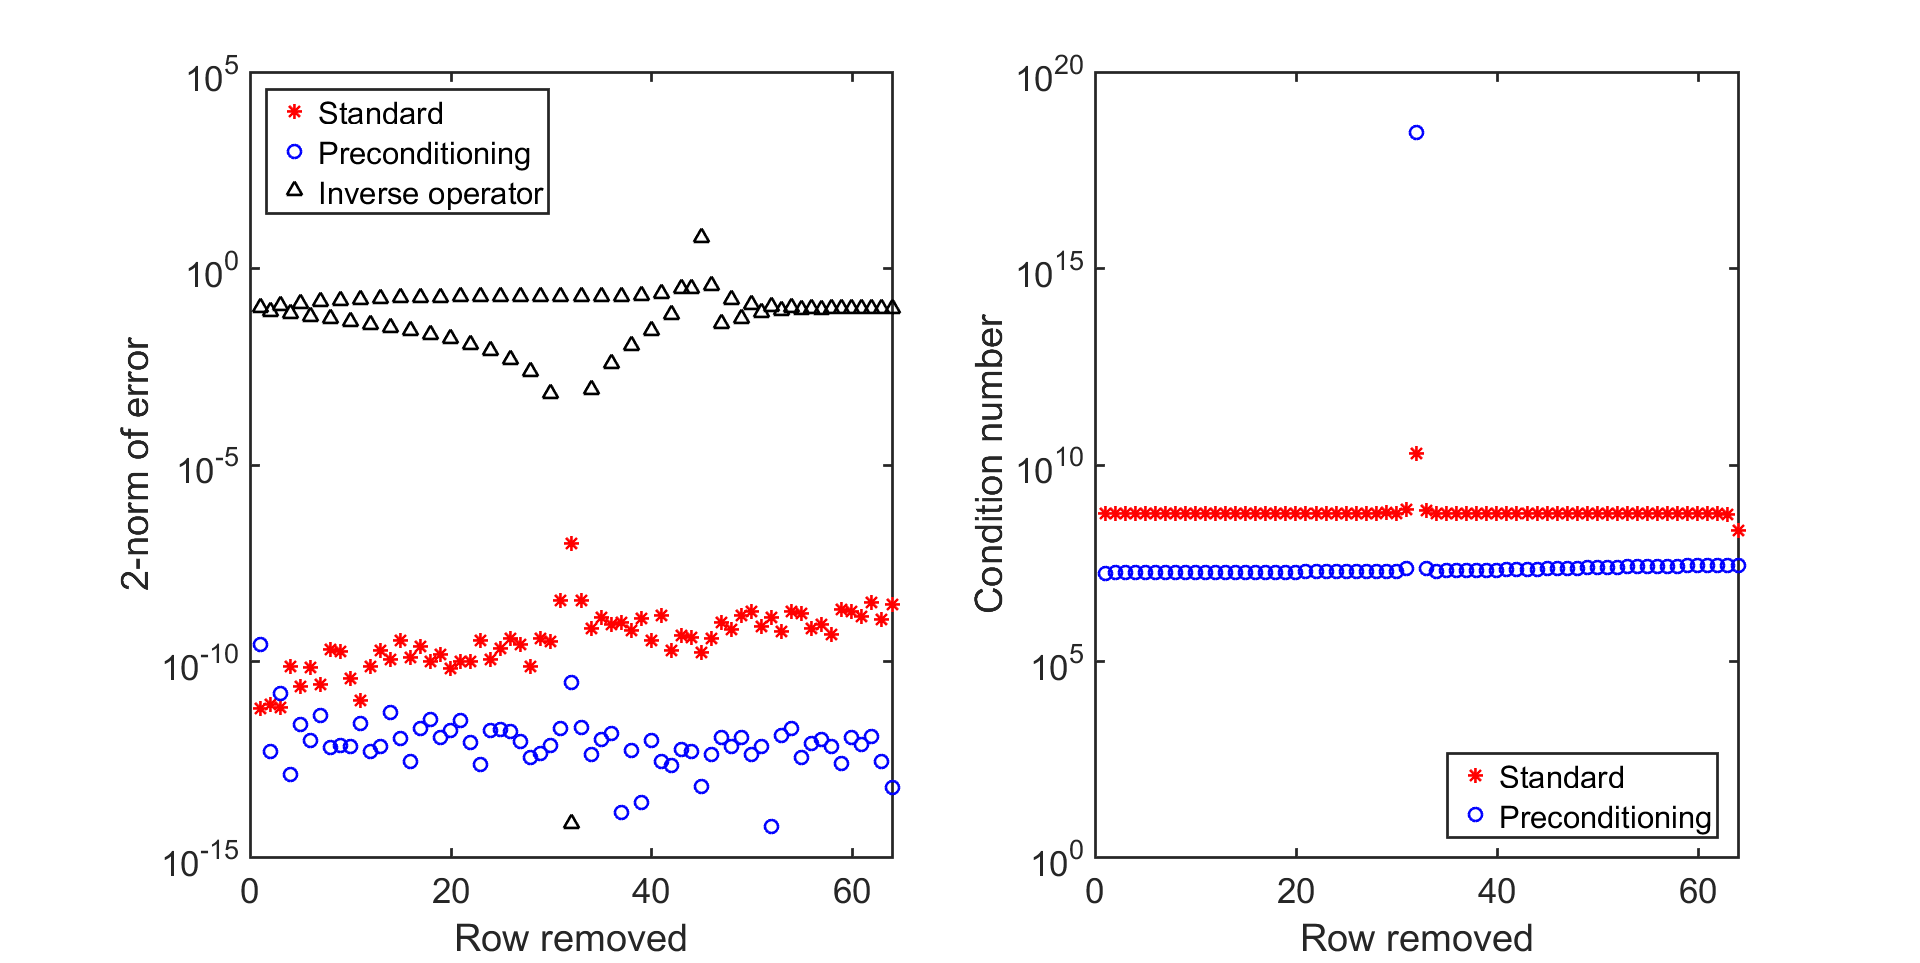
\includegraphics[width=\textwidth]{example_SingCoeffs_02.png}
\caption{Error (left) and condition number (right) for the standard, modal preconditioning and inverse operator methods in solving equation (\ref{exSing}) as a function of the second row removed. In this case, $V = \{1, x_k \}$ where $k$ runs from 1 to $N = 64$.}
\label{fig:SingCoeffs V}
\end{figure}

The left of figure \ref{fig:SingCoeffs V} shows several interesting features.
The inverse operators provides the worst accuracy for all choices of $V$ except $V = \{1, 0\}$, where it provides one of the best.
For this choice of $V$, the condition numbers of the systems for both standard and modal preconditioning jump up several orders of magnitude, as does their error.

For the standard method, best accuracy is attained for $V = \{1, x_1\}$.
Best accuracy for modal preconditioning is attained near $V = \{1, -1\}$.
For simplicity, we will not consider the actual minimum, occurring somewhere between -1 and 0.

\begin{figure}
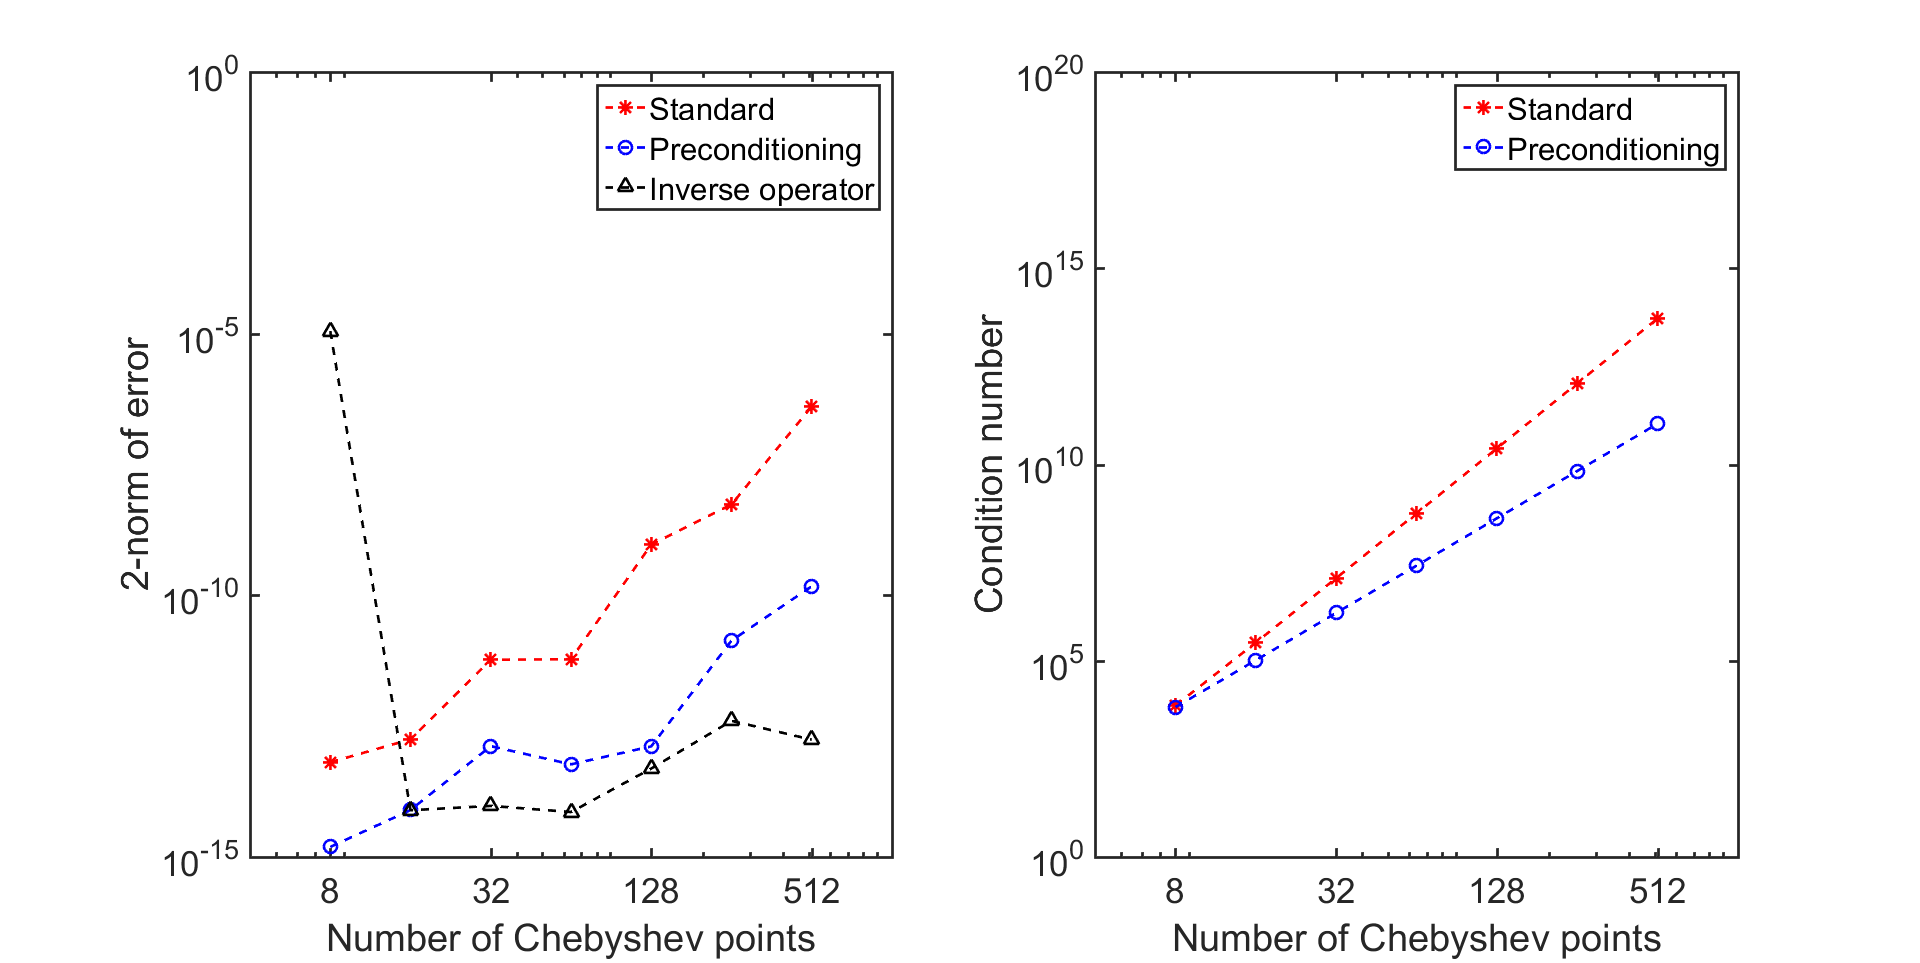
\includegraphics[width=\textwidth]{example_SingCoeffs_03.png}
\caption{Error (left) and condition number (right) for the standard, modal preconditioning and inverse operator methods in solving equation (\ref{exSing}) as a function of $N$. $V$ is chosen to be $\{1, x_1\}$ for the standard method, $\{1, -1\}$ for modal preconditioning and $\{1, 0\}$ for inverse operators.}
\label{fig:SingCoeffs N}
\end{figure}

Using these choices of $V$ that appear to maximize accuracy, the methods are tested for several values of $N$.
Figure \ref{fig:SingCoeffs N} shows the results for all three methods with $V = \{1, x_1\}$ for the standard method, $\{1, -1\}$ for modal preconditioning and $\{1, 0\}$ for inverse operators.

For almost all $N$ inverse operators provide the greatest accuracy.
It also proves the most robust to increasing $N$.
The modal preconditioning also shows an improvement of approximately two orders of magnitude over the standard method.
The condition number for preconditioning increases only slightly less than that of the standard method with increasing $N$.

It is curious that $V = \{1, 0\}$ should be the best choice for the inverse operators,
as there is no linear combination of the two homogeneous solutions that satisfies equation (\ref{homog solns}).
Any combination that satisfies $P(0) = 0$ also has $P'(0) = 0$.
It should be noted that this choice of $V$ effectively removes the singularity.

In practice, using the exact derivatives of the homogeneous solutions to compute $R$ causes singularities for this $V$.
The above results are obtained by using the Chebyshev differentiation matrix $D$ to calculate approximate derivatives.
It seems that by allowing some small error in the value of the derivatives, the matrix $R$ can take advantage of removing the singularity.

\section{5th order example with constant coefficients}

The preconditioning reduces the effects of the highest order numerical differentiation, while the inverse operator reduces the effects of all orders.
Therefore, the inverse operator should produce superior results when used on an example where the second highest order numerical differentiation matrix is badly conditioned.

Consider the following fifth order example:
\begin{equation} \label{ex5th}
u^{(5)}(x) + u^{(4)}(x) - u'(x) - u(x) = f(x)
\end{equation}
with $f(x)$ chosen such that $u(x) = \sin(x^2)$, Dirichlet and Neumann boundary conditions at $x=\pm 1$ as well as the second derivative set at the boundary $x = 1$.

The fundamental set of solutions for this problem is straightforward to find:
\begin{equation}
P_1(x) = \sin(x), \quad P_2(x) =\cos(x), \quad P_3(x) = e^x, \quad P_4(x) = e^{-x}, \quad P_5(x) = x e^{-x}.
\end{equation}

The Birkhoff preconditioning will reduce the effects of the fifth order differentiation matrix, but not those of the fourth order matrix.
In contrast, the inverse operator will remove the effects of all differentiation matrices.

\begin{figure}
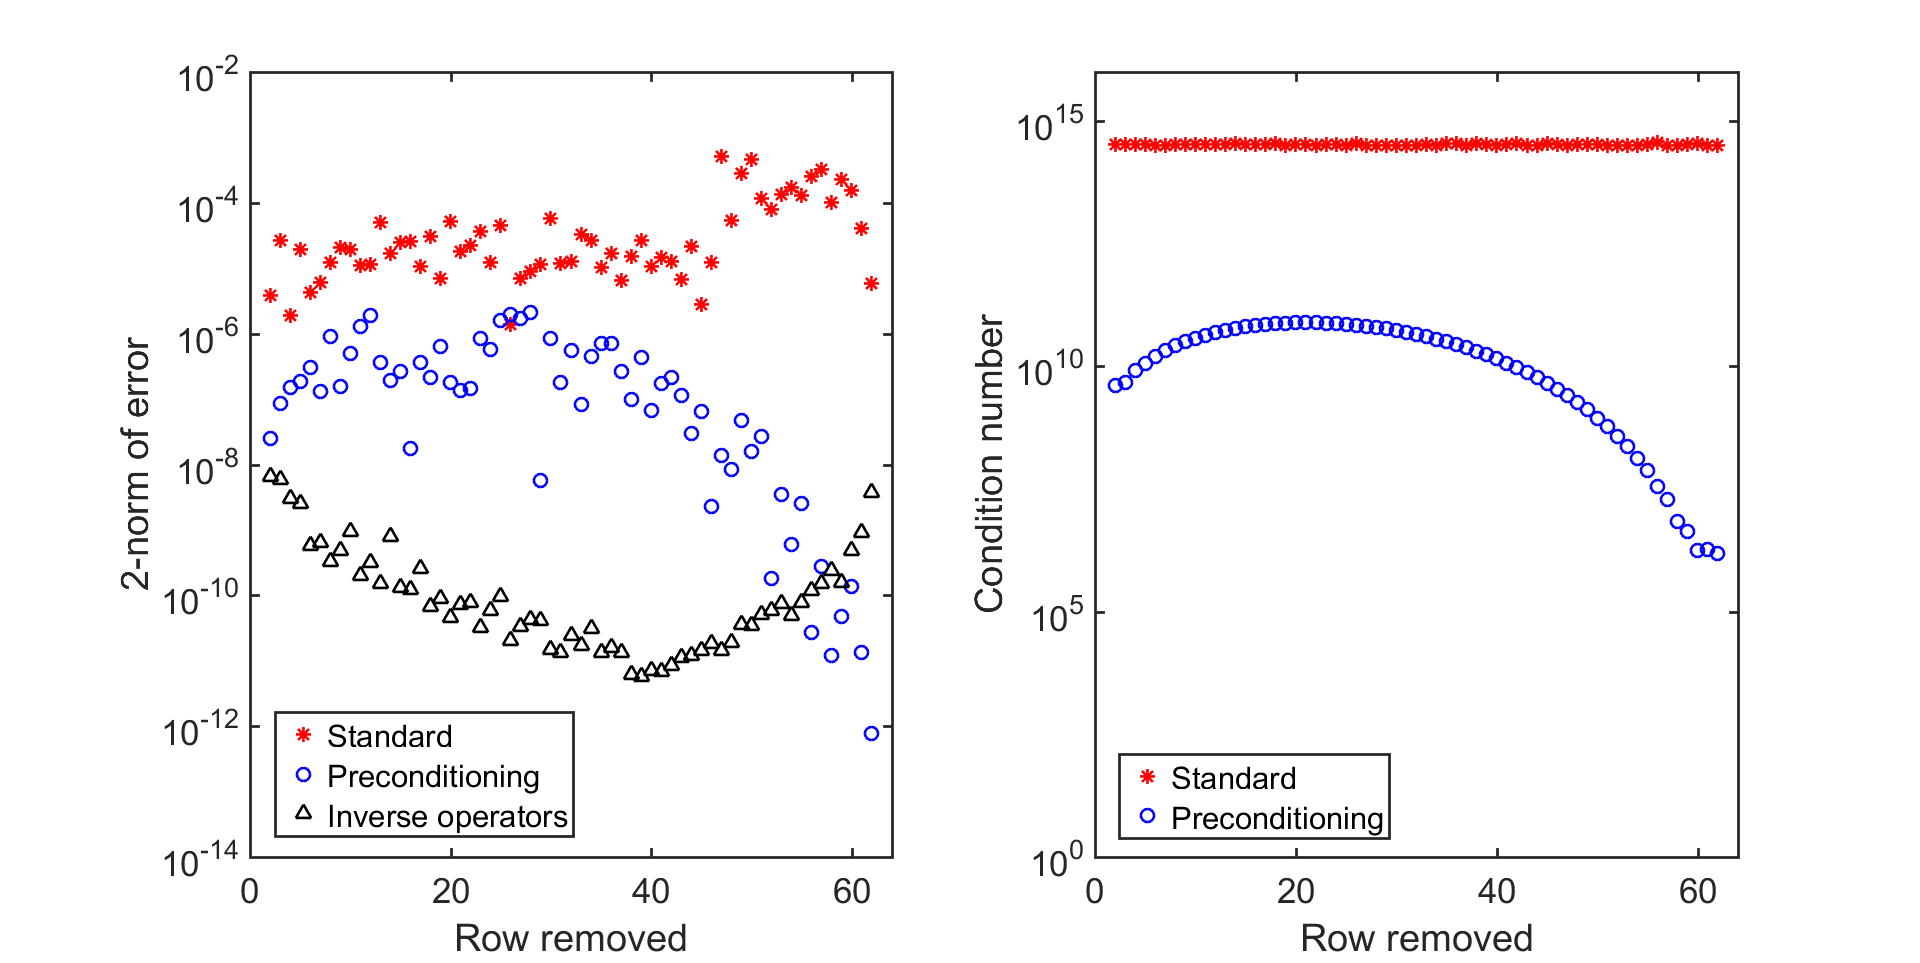
\includegraphics[width=\textwidth]{example_5thCC_V.png}
\caption{2-norm of error (left) and condition number of systems (right) in solving equation (\ref{ex5th}) for $N = 64$ as a function of central row removal. In this case, $V = \{ 1, x_1, x_k, x_{N-1}, -1 \}$ where $k$ runs from 2 to $N-2$.}
\label{fig:ex5thCC V}
\end{figure}

Figure \ref{fig:ex5thCC V} shows the results of solving equation (\ref{ex5th}) for $N = 64$ for various choices of $V$.
Inverse operators show the best results for more choices of $V$, but preconditioning provides the best accuracy overall, with $V = \{1, x_1, x_{N-2}, x_{N-1}, -1\}$.
Best results with inverse operators occurs for row removal near $V = \{1, x_1, 0, x_{N-1}, -1\}$.
Results for the standard method have no apparent relationship with the choice of $V$.

Condition numbers for the standard and preconditioned systems are shown on the right side of figure \ref{fig:ex5thCC V}.
The condition number for the standard method is nearly constant for all tested choices of $V$.
The condition number for the preconditioned system closely matches the shape of the error in the left of the figure.

\begin{figure}
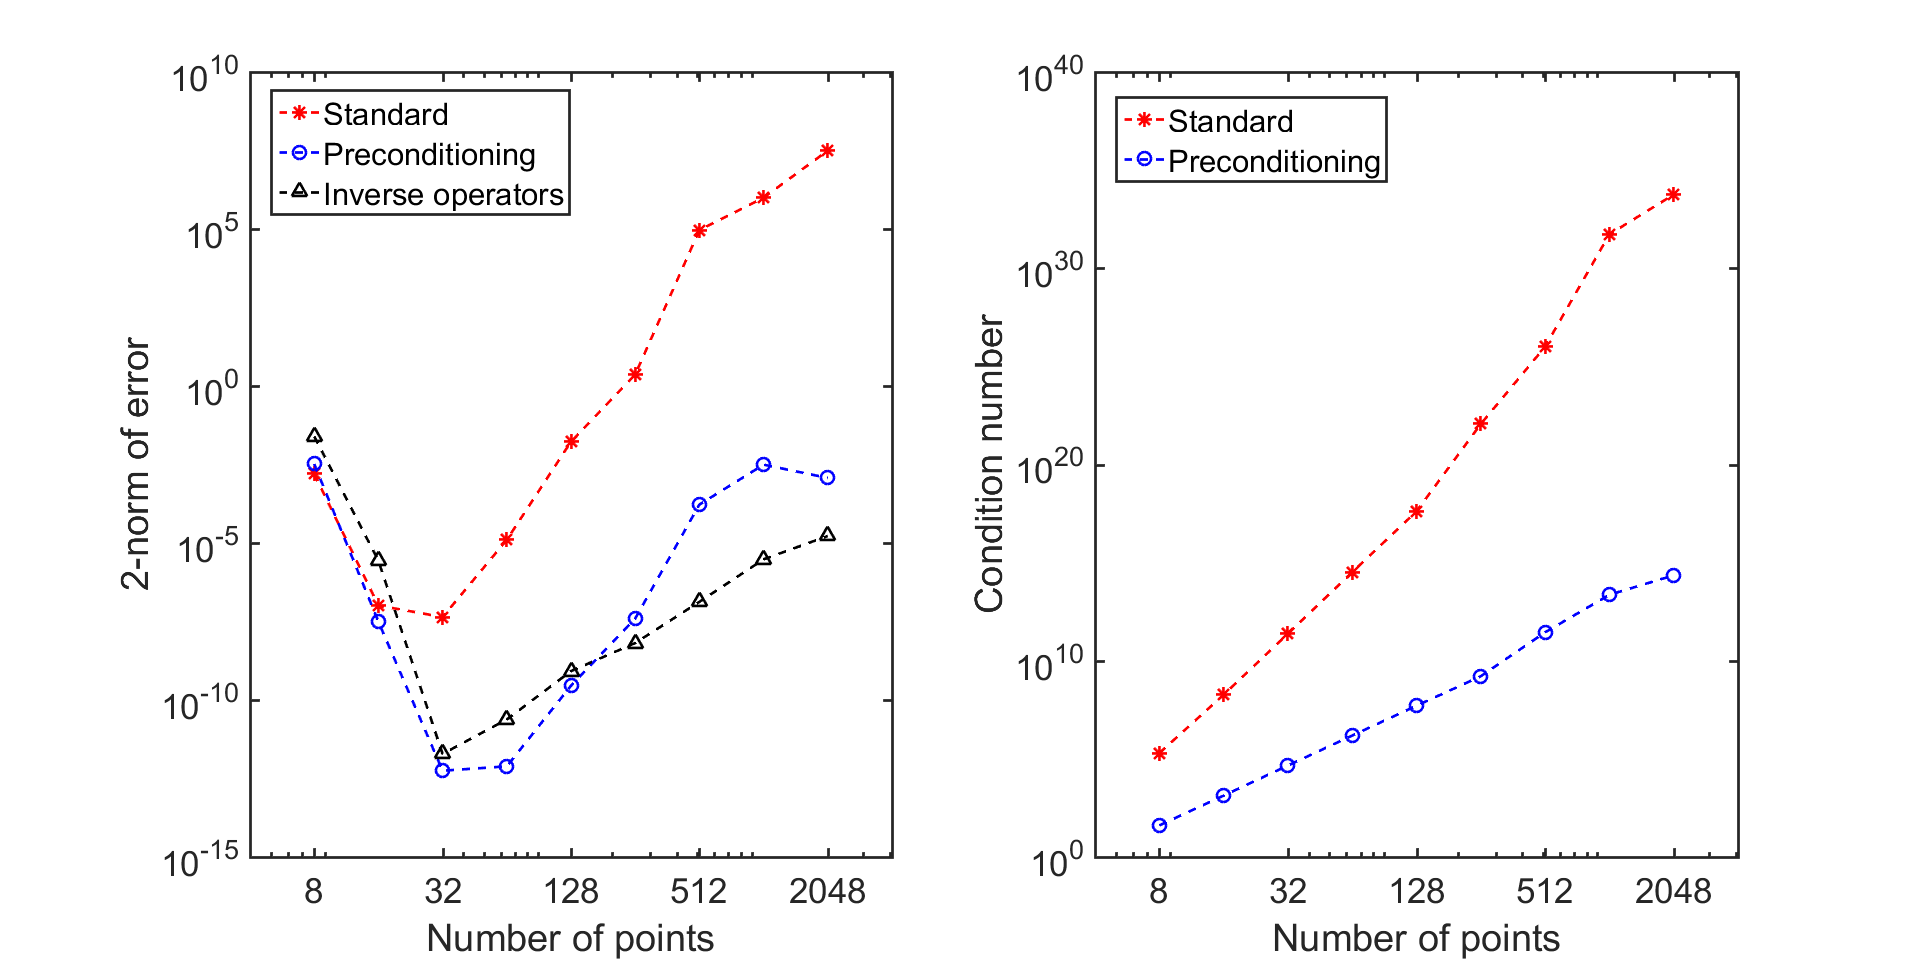
\includegraphics[width=\textwidth]{example_5thCC_N.png}
\caption{2-norm of error (left) and condition number of systems (right) in solving equation (\ref{ex5th}) for various $N$. $V$ is chosen to be $\{ 1, x_1, 0, x_{N-1}, -1\}$ for the standard method and inverse operators, and $\{1, x_1, x_{N-2}, x_{N-1}, -1\}$ for the preconditioning.}
\label{fig:ex5thCC N}
\end{figure}

Figure \ref{fig:ex5thCC N} shows the results of solving equation (\ref{ex5th}) for several values of $N$ using $V = \{ 1, x_1, 0, x_{N-1}, -1\}$ for the standard method and inverse operators, and $\{1, x_1, x_{N-2}, x_{N-1}, -1\}$ for the preconditioning.
The standard method struggles to find an accurate solution, especially for large $N$.
The preconditioning provides the most accurate results for $N<256$, after which the inverse operators is more accurate.

The condition number of the preconditioned system increases slower than the standard system.
However, for sufficiently large $N$ the system is still ill-conditioned.
It is for these values of $N$ that the inverse operators provide the best results, as they arrive at the answers without solving an ill-conditioned system.
Best accuracy is still obtained between $N = 32$ and $N = 64$ using the preconditioned system.
Therefore, the inverse operators method is only preferable when high resolution is required.

%\begin{figure}
%\includegraphics[width=\textwidth]{example_5th_N.png}
%\caption{Results for solving equation (\ref{ex5th}) using the standard method, Birkhoff preconditioning, and inverse operators using both exact and computed derivatives of the homogeneous solutions, varying the number of points used from $N = 8$ to 512.}
%\label{fig:ex5th N}
%\end{figure}
%
%Figure \ref{fig:ex5th N} shows the maximum error in solving equation (\ref{ex5th}) as a function of the number of Chebyshev points, $N$.
%The first, second, middle, second to last, and last rows are removed and replaced with boundary conditions.
%
%The inverse operator gives distinct advantages, as seen in figure \ref{fig:ex5th N}.
%The standard method and Birkhoff preconditioning have similar upward trends past $N = 32$.
%Likewise, the maximum errors for the inverse operator methods run parallel between $N = 32$ and $N = 256$.
%Using exact derivatives gives an improvement of approximately an order of magnitude.
%
%Not only do the inverse operator methods provide more accurate results for $N$ greater than 32, they appear to be more robust towards round-off error.
%Although using the computed derivatives requires less input information, using the exact derivatives gives a significant boost to accuracy.
%
%\begin{figure}
%\includegraphics[width=\textwidth]{example_5th_row.png}
%\caption{Results for solving equation (\ref{ex5th}) using the standard method, Birkhoff preconditioning, and inverse operators using both exact and computed derivatives of the homogeneous solutions, varying the third row replaced to accomodate boundary conditions.}
%\label{fig:ex5th row}
%\end{figure}
%
%Figure \ref{fig:ex5th row} shows the maximum error in solving equation (\ref{ex5th}) as a function of the row removed to accomodate the third boundary condition.
%In addition to this row, the first, second, second to last, and last rows are removed to accomodate the first, second, fourth, and fifth boundary conditions, respectively.
%For this figure, $N = 128$.
%
%It is clear that the Birkhoff preconditioning is improved by removing rows closer to the end of the matrix.
%In fact, it appears that Birkhoff preconditioning is as effective or superior to the inverse operator method using computed derivatives.
%However, there is currently no a priori way of knowing which row will produce these superior results, for any method.
%It should also be noted that the minimum of the inverse operator method using exact derivatives is still lower than that for Birkhoff preconditioning.

\section{5th order example with non-constant coefficients}

Consider the following example from Wang et al. \cite{wang2014well}:
\begin{equation} \label{exWang}
u^{(5)}(x) + \sin(10x) u'(x) + x u(x) = f(x), \quad u(\pm 1) = u'(\pm 1) = u''(1) = 0
\end{equation}
where $f(x)$ is chosen such that the solution is $u(x) = \sin^3(\pi x)$.

The fundamental set of solutions will pose a challenge to find.
Instead, one can use the null space of the matrix for the standard method without boundary conditions.
This matrix is represented by $\bar{A}$ in Chapter \ref{intro}.
However, round-off error can cause the calculated null space to be of higher dimension than the order of the problem.

As a second alternative, it can be noted that the fundamental set of solutions solves the system:
\begin{equation}
A P = \bar{I}
\end{equation}
where $\bar{I}$ is the matrix formed by the columns of the identity matrix associated with the points in $V$.
Using this approach means the standard method must be used to construct the inverse operator $R$.
This removes many of the benefits of using $R$.

\begin{figure}
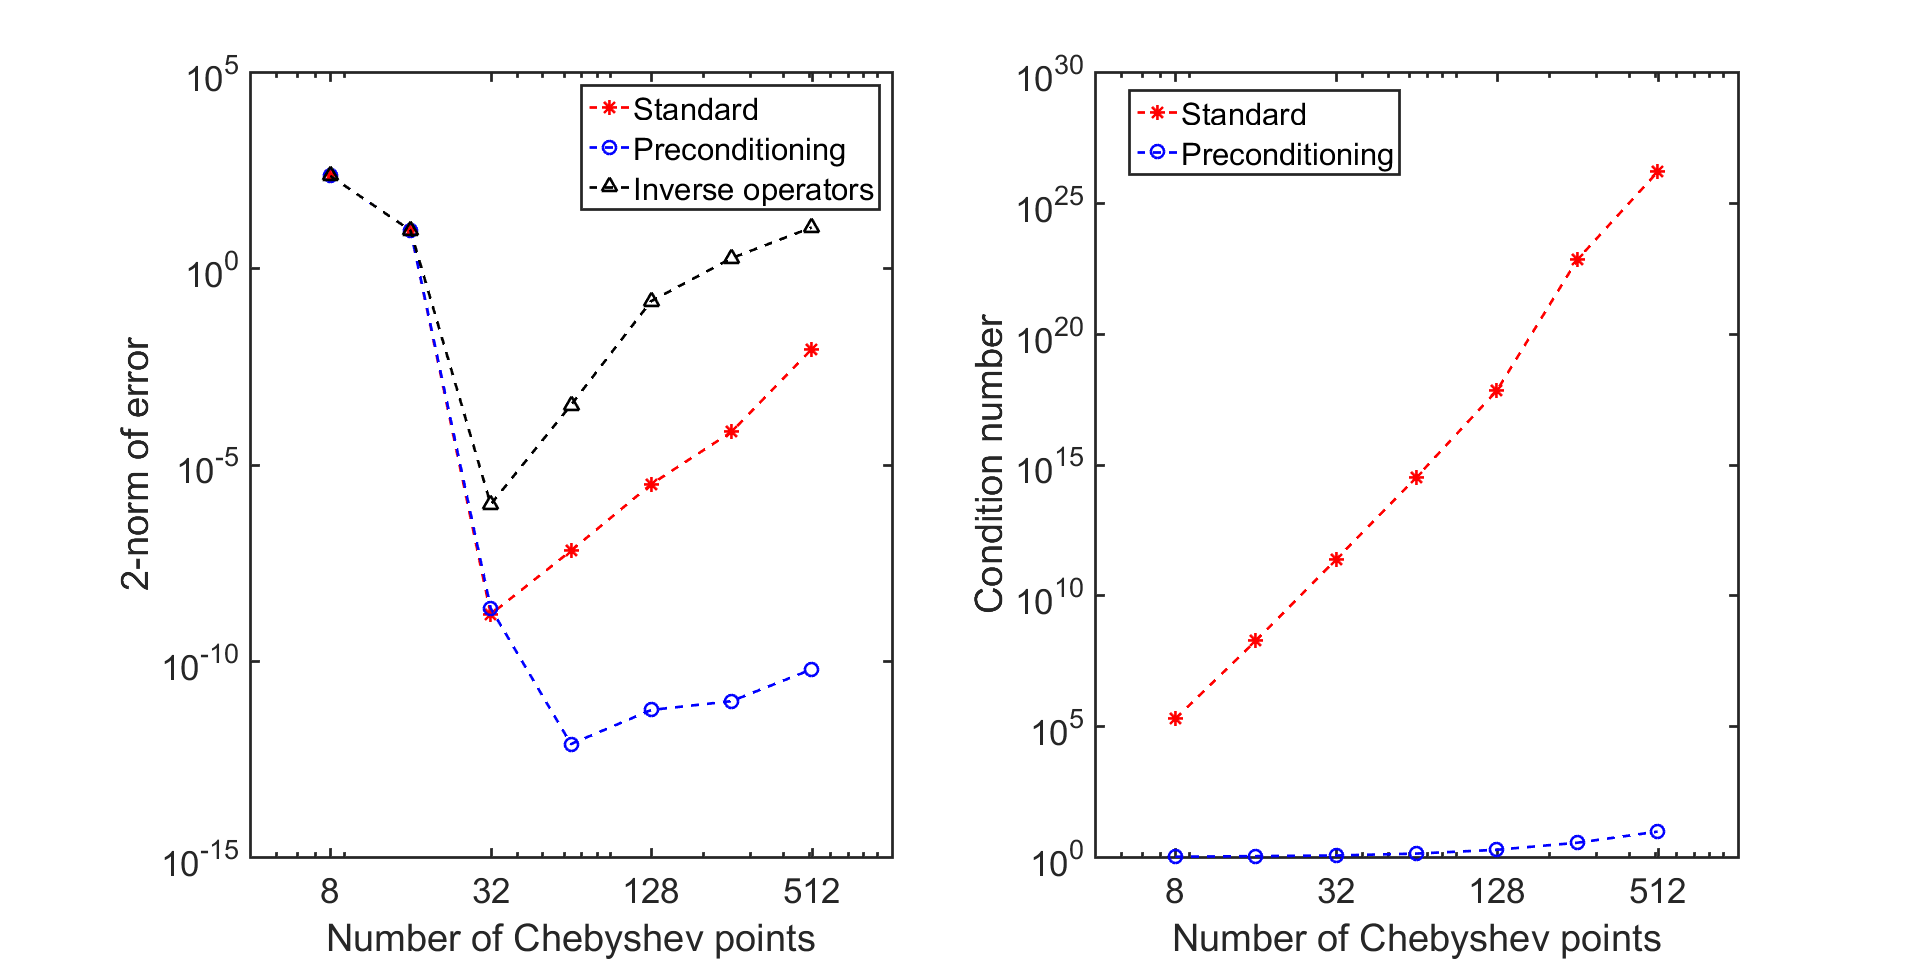
\includegraphics[width=\textwidth]{example_Wang5th_N.png}
\caption{2-norm of error in solving equation (\ref{exWang}) (left) and condition number of systems used to solve equation (\ref{exWang}) (right) as functions of the number of Chebyshev points, $N$. Since the solution found using inverse operators is arrived at through matrix multiplication, the condition number is 1.}
\label{fig:Wang5 N}
\end{figure}

Figure \ref{fig:Wang5 N} shows the results for various $N$ using $V = \{-1, x_{N-1}, 0, x_1, 1\}$.
The left side shows the 2-norm of the error, while the right side shows the condition number of the relevant system.
The condition number of the inverse operators is not shown as it uses only matrix multiplication, and so has a condition number of 1.

It is clear that the inverse operators should not be used for this problem, as there are no gains in accuracy and a system must still be solved.
The preconditioning removes the largest source of round-off error, leaving a significantly smaller condition number.
Not only is the preconditioning more accurate for all values of $N$, it shows greater robustness to increasing $N$.

\begin{figure}
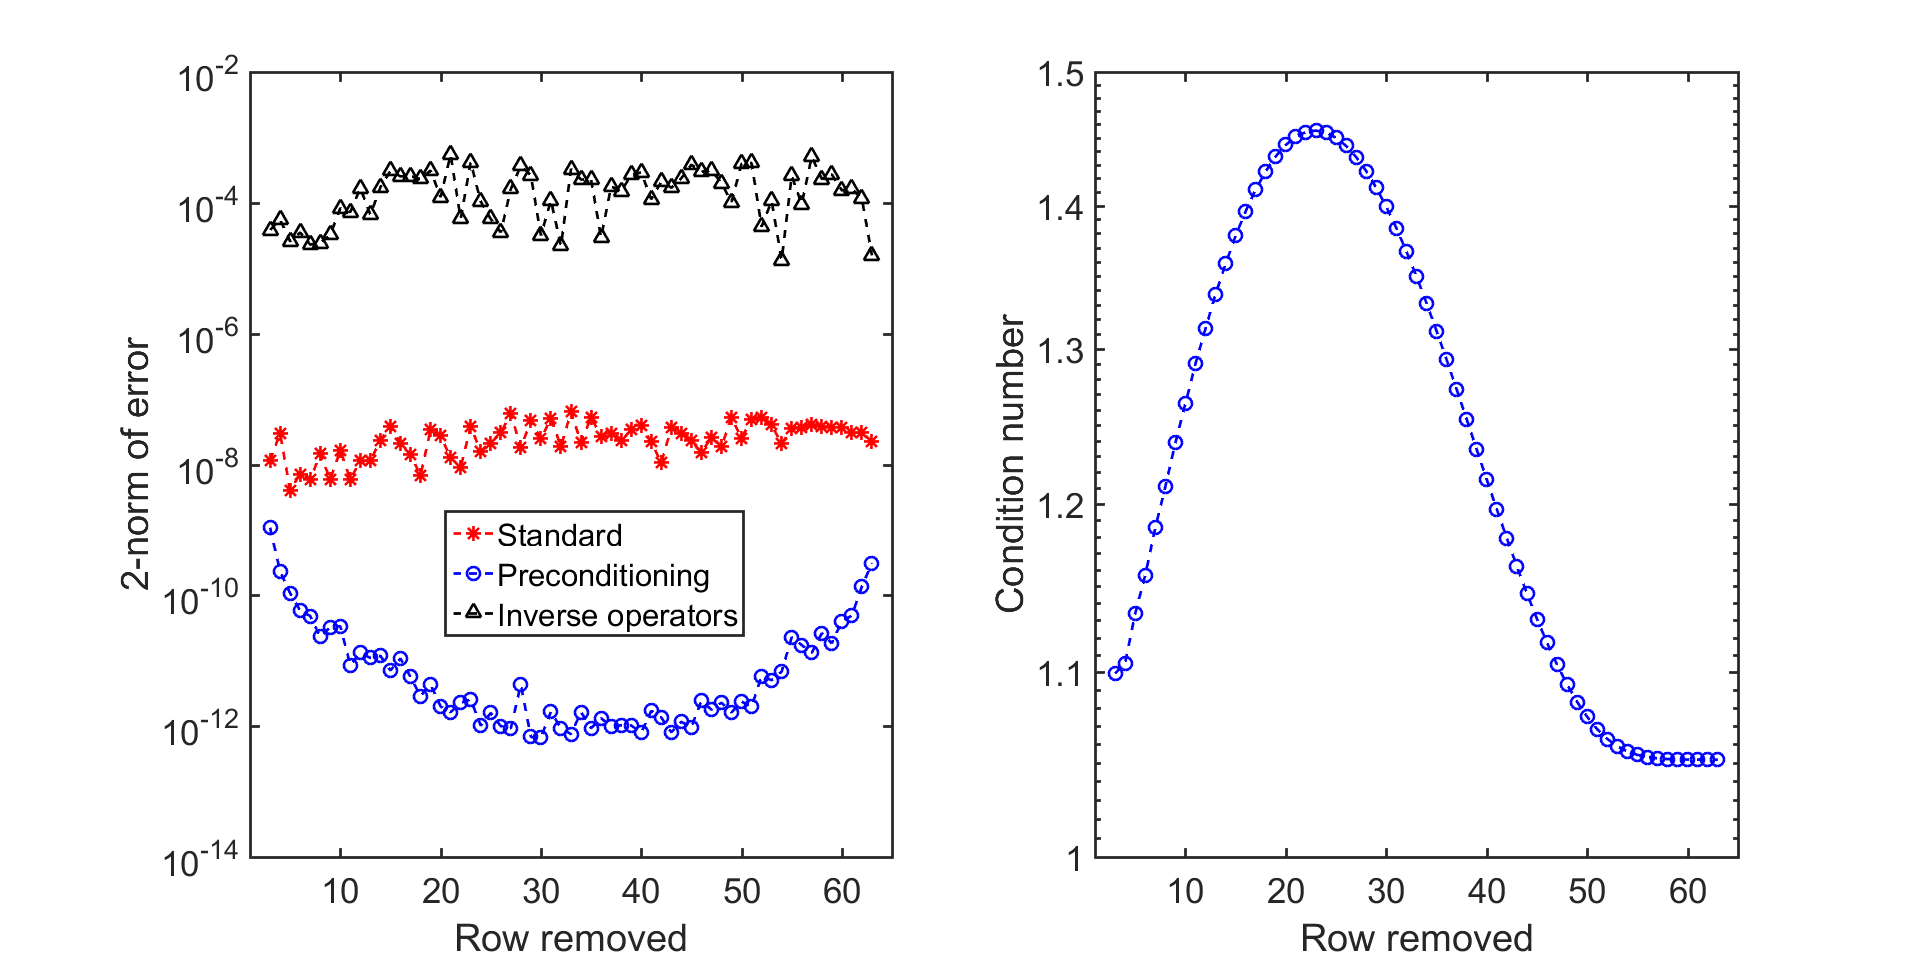
\includegraphics[width=\textwidth]{example_Wang5th_V64.png}
\caption{2-norm of error in solving equation (\ref{exWang}) (left) and condition number of the preconditioned system (right) as functions of the central row removed for $N = 64$.}
\label{fig:Wang5 V}
\end{figure}

Figure \ref{fig:Wang5 V} shows the results for $N = 64$ and $V = \{ -1, x_{N-1}, x_k, x_1, 1\}$ where $k$ varies from 2 to $N -2$.
The 2-norm of the error is presented on the left for all three methods.
No apparent trend is seen for inverse operators or the standard method.
The preconditioning shows a preference for $x_k$ near 0.
The right side of the figure shows the condition number of the preconditioning.
While greatest accuracy is found by removing rows near the centre, this leads to the largest condition number.

\section{Nonlinear example}

The following nonlinear differential equation is taken from Ascher et al. \cite{AMR}:
\begin{equation} \label{exAscher}
u^{(4)}(x) = u'(x) u''(x) - u(x) u^{(3)}(x), \quad u(\pm 1) = u'(-1) = 0, \quad u'(1) = 1 .
\end{equation}
The solution can be found using an iterative method.

Construct the standard matrix $A$ and the preconditioning matrix $B$ for fourth order differentiation with Dirichlet and Neumann boundary conditions.
Choose $V = \{-1, x_{N-1}, x_1, 1\}$.
Let $U_0 = 0$ be the initial guess, and $U_n$ be the solution at the $n$--th iteration.
The right hand side of the $n+1$--th system can be written as:
\begin{equation}
F = ( DU_n )( D^2 U_n ) - U_n ( D^3 U_n )
\end{equation}
with the rows prescribed by $V$ replaced with boundary conditions.
The solution at the $(n+1)$--th iteration is then:
\begin{equation}
\begin{aligned}
(i) & \ U_{n+1} = A \backslash F \\
(ii) & \ U_{n+1} = B F
\end{aligned}
\end{equation}
where $(i)$ is the standard method and $(ii)$ is the preconditioned method.

Note that the inverse operators are excluded from this example.
As has been explained, for linear operators representing differentiation the inverse operator matrix $R$ is theoretically equivalent to the preconditioning matrix $B$.
The differences between the two are dealt with in Chapter \ref{compare}.

\begin{figure}
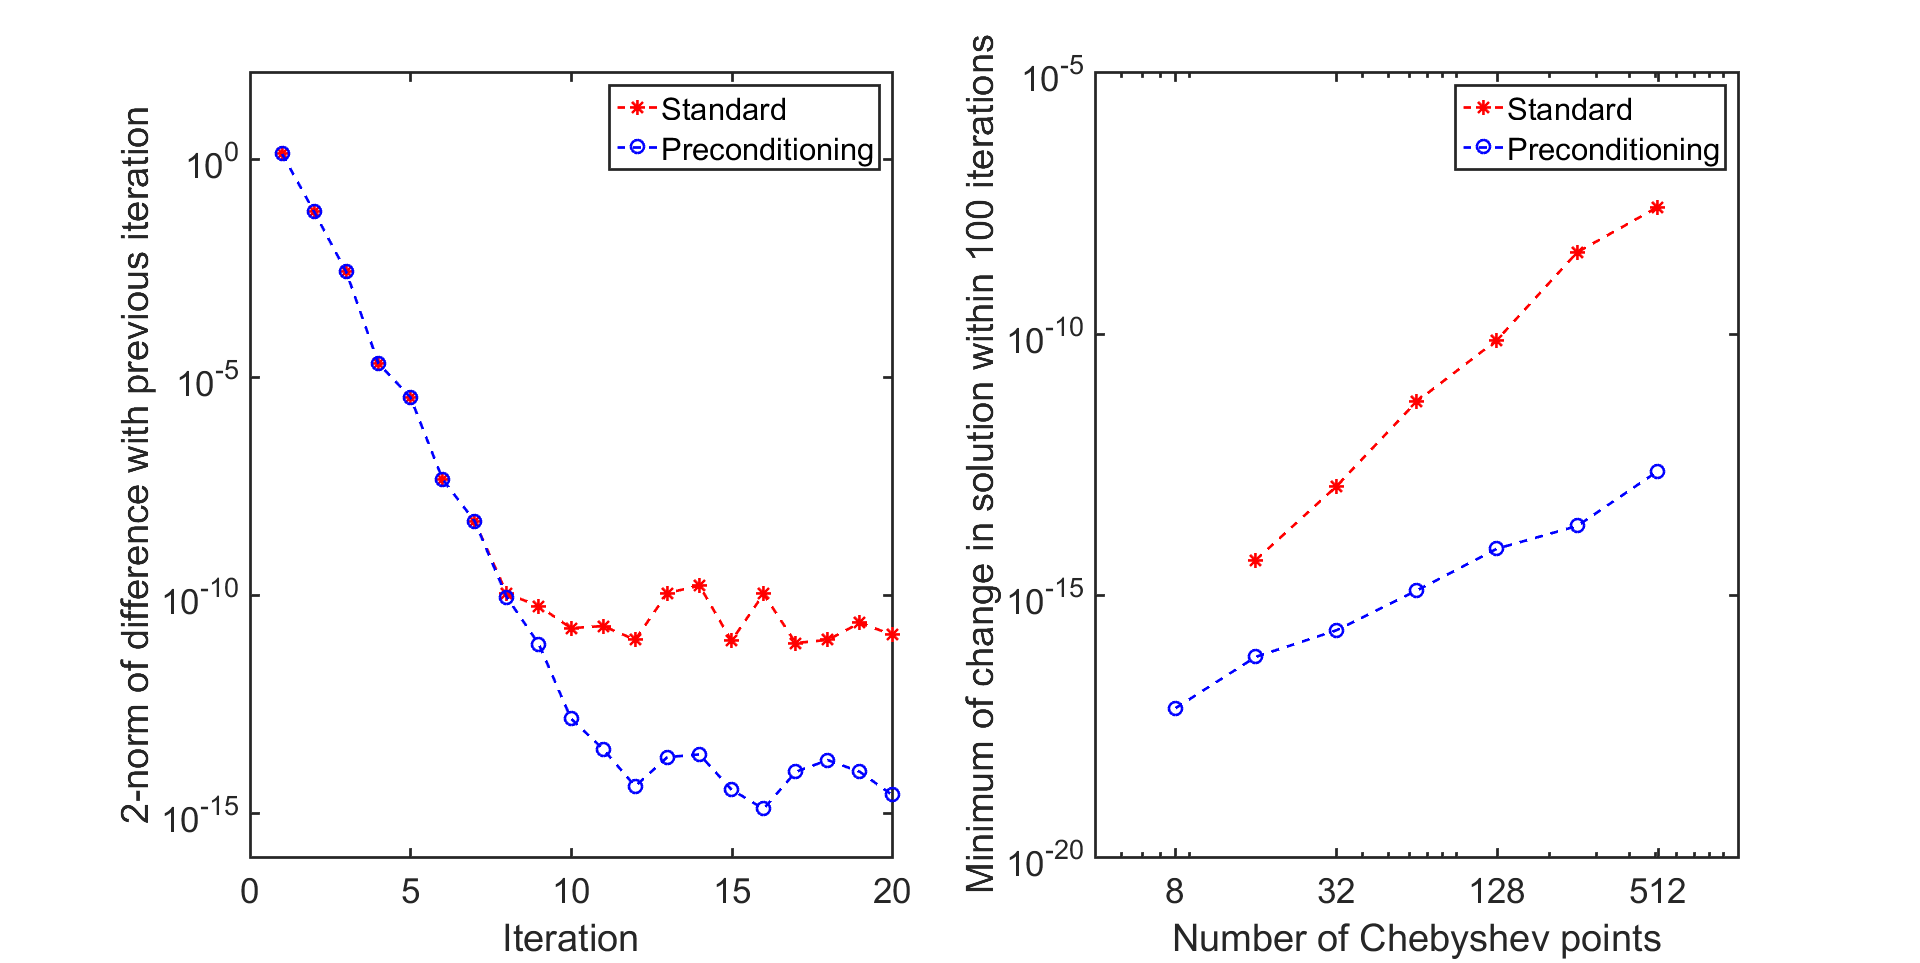
\includegraphics[width=\textwidth]{example_AscherNonlinear.png}
\caption{2-norm of the change in solutions over 20 iterations for $N = 64$ (left) and minimum change in solutions within 100 iterations for various $N$ (right).}
\label{fig:AscherNonlinear}
\end{figure}

Figure \ref{fig:AscherNonlinear} shows the results of using these two iterative methods in solving equation (\ref{exAscher}).
For early iterations, the two methods show identical results.
However, the preconditioned system is able to improve its solution by several orders of magnitude, 
while consecutive iterates of the standard method constantly change by around $1e-10$, as measured by the 2-norm.
The right side of the figure shows that the preconditioned system is more robust to increasing values of $N$ than the standard method.

The condition number for the matrix $A$ grows as roughly $\mathcal{O}(N^9)$.
As such, using the standard method requires solving several ill-conditioned systems.
This is circumvented in the preconditioned case, as only matrix multiplication is used.

Suppose the example instead used a more general linear operator $\mathcal{L}$ in place of fourth order differentiation.
In this case, the preconditioning would require solving several systems, though they would still be better conditioned than the standard method.
The inverse operator matrix would no longer be the same as the preconditioning matrix.
Using the inverse operator matrix would require only matrix multiplication, and may prove more robust than the preconditioning for such a problem.

\section{PDE example}

Consider the one dimensional diffusion equation:
\begin{equation}
u_t = \mu u_{xx}, \quad u(x,0) = g(x)
\end{equation}
with homogeneous Dirichlet boundary conditions.
Using the backward Euler method, the following time step may be used:
\begin{equation}
(I - \mu \Delta t D^2) U^{n+1} = U^n
\end{equation}
where $\Delta t$ is the size of each time step and $D^2$ are differentiation matrices of order 2 respectively.

Let $A$ be the matrix $I - \mu \Delta t D^2$ with rows prescribed by the set $V = \{ 1, -1 \}$ replaced with boundary conditions.
Let $G$ be the vector of the initial condition $g(x)$ evaluated at the Chebyshev points (\ref{CGL}), with the elements prescribed by $V$ replaced with zeros.
This gives the numerical solution at time $t_n = n \Delta t$ as $U^n = (A^{-1})^n G$.

If the PSIM is constructed for second order differentiation with Dirichlet boundary conditions, the time step can instead be written as:
\begin{equation}
(B - \mu \Delta t \tilde{I}) U^{n+1} = B U^n
\end{equation}
noting that $\tilde{I}$ is the identity matrix with the rows prescribed by $V$ replaced with zeros so as not to interfere with the boundary conditions.
For inhomogeneous boundary conditions, care must be taken as to the sign of the first and last element in $U^n$.

Preconditioning with the PSIM is done to reduce the condition number of the matrix $A$.
It does so by removing the highest order differentiation matrix.
Incidentally, this is the largest source of round-off error in constructing the system.
In this example, if $\mu \Delta t$ is small the effects of the matrix are already mitigated by multiplication by a small number.
In fact, if $B$ itself is poorly conditioned, for sufficiently small $\mu \Delta t$, preconditioning may lead to an even more poorly conditioned time step.

To construct the inverse operator matrix, the differential operator must be rewritten to isolate the highest order differentiation matrix:
\begin{equation}
\mathcal{L} = \left ( \frac{d}{dx} \right )^2 - \frac{1}{\mu \Delta t}.
\end{equation}
The fundamental solution set is then $\left \{ \sinh \left ( \frac{x}{\sqrt{\mu \Delta t}} \right ), \cosh \left ( \frac{x}{\sqrt{\mu \Delta t}} \right ) \right \}$.
The time step can then be represented by:
\begin{equation}
U^{n+1} = (-R / \mu \Delta t) U^n .
\end{equation}

For small $\mu \Delta t$, the fundamental solution set contains a function that grows exponentially away from $x=0$.
This poses a threat of overflow and amplification of round-off error in calculating the matrix $R$.
Ideally, the inverse operator should only be employed for $\mu \Delta t$ on the order of 1.

In Chapter \ref{ch:spectra} the exact eigenvalues of several problems were found.
For this problem, the eigenvalue problem for $V = \{-1, 1\}$ becomes:
\begin{equation}
-a u''(x) + u(x) = \lambda u(x), \quad u(\pm 1) = 0, 
\end{equation}
where $a = \mu \Delta t$.
This ultimately leads to the eigenvalues $\lambda = 1 + a ( k \pi /2 )^2$ for $k \in \mathbb{N}$.
For $a>0$, all eigenvalues are greater than 1 and there are no stability issues arising from the exact eigenvalues.

\begin{figure}
\includegraphics[width=\textwidth]{example_diff_stabAll.png}
\caption{Largest eigenvalue of the matrices $A^{-1}$, $(B - \mu \Delta t I)^{-1} B$ and $R$ for various values of $\mu \Delta t$.}
\label{fig:stabR}
\end{figure}

With exact eigenvalues for the forward problem always greater than 1, the eigenvalues of $R$ are expected to all be less than or equal to 1.
Despite this, figure \ref{fig:stabR} shows that the matrix $R$ has eigenvalues greater than 1, and thus stability issues, for small $\mu \Delta t$.
The matrix $R$ cannot be used for $\mu \Delta t< 0.04$.
The standard method and preconditioning show no instabilities due to eigenvalues.

%change problem to one with forcing, then find exact solution

%--------------------------------------------
% 		Arbitrary collocation points
%--------------------------------------------

%Taken directly from paper, need to fix for thesis

\chapter{Arbitrary collocation points}
\label{sec:further}

The methods described above can be used more generally to find solutions on points other than the Chebyshev points.
Given a set of points $Y = \{y_0, y_1, ... , y_N\}$ and a matrix equation $A \vec{U} = \vec{F}$ on the Chebyshev points,% of the form of equation (\ref{matrix ODE}),
define the following matrices element-wise:
\begin{equation}
\mathcal{T}_{ij} = \cos \left ( \frac{i j \pi}{N} \right ), \quad \mathcal{T}^{-1}_{ij} = \frac{2}{c_i c_j N} \mathcal{T}_{ij}, \quad L_{ij} = T_j(y_i)
\end{equation}
where $c_i$ are the weights from equation (\ref{weights}) and $T_j(x)$ are the Chebyshev polynomials.
The operation $\mathcal{T}^{-1} A \mathcal{T} = A_{\mathcal{T}}$ moves the matrix $A$ to the spectral space of the Chebyshev polynomials.
$A_{\mathcal{T}}$ is a matrix of coefficients of Chebyshev polynomials associated with the ODE operator $A$.
The product $L A_{\mathcal{T}}$ is therefore the evaluation of $A$ at the points $Y$.
It remains to decompose the solution into coefficients of the Chebyshev polynomials evaluated on $V$.
This is achieved with the inverse of $L$, $L^{-1}$.
Thus the matrix equation on the set of points $Y$ is $A_Y \vec{U_Y} = \vec{F_Y}$ where $A_Y = L \mathcal{T}^{-1} A \mathcal{T} L^{-1}$.
The definition of $\vec{U_Y}$ and $\vec{F_Y}$ can be found directly:
\begin{equation}
A \vec{U} = \vec{F} \implies A \mathcal{T} L^{-1} L \mathcal{T}^{-1} \vec{U} = \vec{F} \implies L \mathcal{T}^{-1} A \mathcal{T} L^{-1} L \mathcal{T}^{-1} \vec{u} = L \mathcal{T}^{-1} \vec{F},
\end{equation}
and so $\vec{U_Y} = L \mathcal{T}^{-1} \vec{U}$ and $\vec{F_Y} = L \mathcal{T}^{-1} \vec{F}$.

The transformation $L \mathcal{T}^{-1} A \mathcal{T} L^{-1} = A_Y$ is linear.
Therefore, if $B A = I$, then $B_Y A_Y = I$.
Thus, the desired property of the preconditioning matrix is maintained on the new set of points $Y$.
However, if the matrix $A_Y$ is constructed on the set $Y$, then $B_Y$ will not satisfy this property.
Specifically, if $D^{(k)}_Y$ is the $k$--th order differentiation matrix on $Y$ and $\tilde{A}_Y$ is the matrix constructed analogously to those in Chapter \ref{intro} then $B_Y$ does not approximate the inverse of $\tilde{A}_Y$.
This is presented in the following lemma.

\begin{lemma}
Let $D^{(k)}_Y$ be the $k$--th order differentiation matrix on the points $Y \neq X$.
Let $\tilde{A}_Y$ be the matrix constructed as in Chapter \ref{intro} for a linear operator with constant coefficients using the matrices $\{ D^{(k)}_Y \}_{k=1}^m$.
Let $A$ be the analogous matrix on the Chebyshev points, and $R$ its inverse.
Then $R_Y = L \mathcal{T}^{-1} R \mathcal{T} L^{-1}$ is not the inverse of $\tilde{A}_Y$.
\end{lemma}

\begin{proof}
First consider $D$ representing first order differentiation on the Chebyshev points.
Let $D_Y$ be the analogous matrix on the points $Y$.
Note that $D_Y = L \mathcal{T}^{-1} D \mathcal{T} L^{-1}$.

Let $A$ result from replacing the $n$--th row of $D$ with the boundary condition.
Likewise, let $\tilde{A}_Y$ result from performing the same operation on $D_Y$.
Let $B$ be the inverse of the matrix $A$.
Then $B_Y$, the transformation of $B$, is the inverse of $A_Y$, the transformation of $A$.
For $B_Y$ to be the inverse of $\tilde{A}_Y$ requires $\tilde{A}_Y = A_Y$.

To show this is not true for a general set of points, consider $Z = D - A$ and $Z_Y$ the transformation of $Z$.
Note that $Z_Y = D_Y - A_Y$, and if $\tilde{A}_Y = A_Y$ then the only non-zero row of $Z_Y$ is the $n$--th row, as this is the only row of $\tilde{A}_Y$ that is not the same as $D_Y$.
Moreover, the only non-zero row of $Z$ is the $n$--th row, as this is the only row of $D$ that is not the same as $A$.

Let $\vec{z}$ be the $n$--th row of $Z$.
Let $\vec{s_i}$ be the $i$--th column of the matrix product $\mathcal{T}L^{-1}$ and $t_{ij}$ the element in the $i$--th row and $j$--th column of $L \mathcal{T}^{-1}$.
Then $Z_Y$ can be written element-wise as:
\begin{equation}
\left ( Z_Y \right )_{ij} = t_{in} \vec{z} \cdot \vec{s_j} .
\end{equation}
Since $\{\vec{s_j}\}$ spans the space $\mathbb{R}^{N+1}$, $\vec{z} \cdot \vec{s_j}$ must be non-zero for at least one $j$.
Thus for the $i$--th row of $Z_Y$ to be zero requires $t_{in} = 0$.

Recall that $L_{ij} = T_j(y_i)$ where $T_j(x)$ is the $j$--th Chebyshev polynomial and $y_i$ a point in the set $Y$.
The rows of $L$ can be decomposed into the rows of $\mathcal{T}$ since these rows span $\mathbb{R}^{N+1}$:
\begin{equation}
L_{ij} =T_j(y_i) = \sum_{k=0}^N \lambda_{ik} T_j(x_k) .
\end{equation}
It can be shown with equation (\ref{ortho}) that $\lambda_{ik} = t_{ik}$.
Note that $T_1(y_i) = y_i = \sum_{k=0}^N t_{ik} x_k$, which implies:
\begin{equation}
T_j(y_i) = T_j( T_1(y_i)) = T_j \left ( \sum_{k=0}^N t_{ik} x_k \right ) = \sum_{k=0}^N t_{ik} T_j(x_k) \quad \forall \quad 0 \leq j \leq N .
\end{equation}
Using the recursive form of the Chebyshev polynomials gives the following equations:
\begin{equation}
\begin{aligned}
T_j(y_i) = & 2 \sum_{k=0}^N t_{ik} y_i T_{j-1}(x_k) - \sum_{k=0}^N t_{ik} T_{j-2}(x_k) \\
= \sum_{k=0}^N t_{ik} T_j (x_k) = & 2 \sum_{k=0}^N t_{ik} x_k T_{j-1}(x_k) - \sum_{k=0}^N t_{ik} T_{j-2}(x_k) \\
 \implies & \sum_{k=0}^N t_{ik} (y_i - x_k) T_{j-1}(x_k) = 0 .
\end{aligned}
\end{equation}
Let $\vec{w_i}$ be defined element-wise as $w_{ik} = t_{ik} (y_i - x_k)$, then $\mathcal{T}_j  \vec{w_i} = 0$ for all $j = 1, ... , N-1$.
Additionally, taking the sum of all $w_{ik}$ gives:
\begin{equation}
\sum_{k=0}^N t_{ik} (y_i - x_k) = v_i \sum_{k=0}^N t_{ik} - \sum_{k=0}^N t_{ik} x_k = y_i \left (\sum_{k=0}^N t_{ik} - 1 \right ) = 0 \implies \mathcal{T}_0  \vec{w_i} = 0 .
\end{equation}
The only non-zero vector that satisfies this is the last column of $\mathcal{T}^{-1}$.
Thus, $\vec{w_i}$ has the form:
\begin{equation}
\vec{w_i} = b_i
\begin{bmatrix}
1/2 \\ -1 \\ 1 \\ -1 \\ \vdots \\ (-1)^N/2
\end{bmatrix}.
\end{equation}

Therefore, if $t_{in} = 0$ then $b_i = 0$ and $t_{ik} (y_i - x_k) = 0$ for all $k$.
This implies $y_i = x_{\ell}$ for some $\ell$, and thus $Y = X$.
As well, if $Y \neq X$, then $y_i \neq x_k$ for at least one $i$ and all $k$.
This implies $b_i \neq 0$ and $t_{in} \neq 0$.

It is straightforward to extend this to higher orders.
For an $m$--th order problem, $m$ rows need to be removed and $Z$ has $m$ non-zero rows.
Therefore, the $i$--th row of $Z_Y$ will have at least $m$ non-zero entries unless $t_{ij}=0$ for at least $m$ choices of $j$.
By above, this implies $t_{ij} = 0$ for all but one $j$ and $y_i = x_\ell$ for some $\ell$.

This can also be extended to matrices $A$ representing linear operators with constant coefficients.
Recall from Chapter \ref{intro} the definition of the matrix $\bar{A}$:
\begin{equation}
\bar{A} = D^{(m)} + \sum_{n=1}^m Q_n D^{(m-n)} .
\end{equation}
For linear operators with constant coefficients, $Q_n$ is a scalar.
The transformation of this matrix is then:
\begin{equation}
\bar{A}_Y = D^{(m)}_Y + \sum_{n=1}^m Q_n D^{(m-n)}_Y .
\end{equation}
Taking $Z = A - \bar{A}$ allows the above proof to be used.

%should try to prove for non-constant coefficient
\end{proof}

Note that if the transformation of $Q_n$ is diagonal with entries $q_n(y_i)$ for all $n$, then the proof would apply more generally.
However, it cannot be shown that this is true for all functions $q(x)$, and so the transformation of $Q_n$ may well be full.
It is then possible, though unlikely, that the fullness of $Z_Y$ in some way compensates for the fullness of the matrices $Q_{n,Y}$.

To construct the actual inverse of the matrix $\tilde{A}_Y$ using the methods described above,
polynomials analogous to the Chebyshev polynomials $T_k(x)$ for the set $Y$ are required.
Specifically, we need polynomials $L_k(x)$ satisfying:
\begin{equation}
\sum_{j=0}^N w_j L_k(y_j) L_n(y_j) = \alpha(k,N) \delta_{k,n}
\end{equation}
where $w_j$ are arbitrary weights.
Additionally, the integrals of $L_k(x)$ are needed.

%% example on Legendre points

%Let $V$ be the Legendre points \cite{wang2014well} and the following problem will be used to test the preconditioning method on these points:
%\begin{equation} \label{legex}
%u'(x) + u(x) = e^{x-1}, \quad u(1)=0.5
%\end{equation}
%which has as its solution $u(x) = 0.5 e^{x-1}$.
%
%In the results that follow, four methods are compared:
%first, the standard method on the Legendre points; % (citation?);
%second, the transformed preconditioner used on the ODE matrix constructed on the Legendre points;
%third, the transformed preconditioning, analogous to equation (\ref{preconditioning method});
%and fourth, the transformed modal approach, analogous to the one described in Wang et al. \cite{wang2014well}.
%
%Note that in the second method, the transformed preconditioner is not an inverse for the highest order differentiation matrix on the Legendre points.
%Thus, the system cannot be simplified (as in the Chebyshev case) by replacing their product with the identity matrix.
%It should also be mentioned that the transformation introduces its own round-off error and effects on condition number.
%Overall, the accuracy and condition number of these methods cannot be expected to -- and in fact do not -- reflect those on the Chebyshev points.
%For proper analogous methods, a preconditioner specific to the Legendre points would be required.
%
%%figure removed
%
%The results for the four methods are presented in figure \ref{fig:legendre}.
%While the transformed preconditioning and modal approach performed best of the four in terms of accuracy, the preconditioning had the greatest reduction in condition number.

%-----------------------------------
%              Conclusion
%-----------------------------------

\chapter{Conclusion}

As stated in Chapter \ref{intro}, differentiation matrices suffer from large round-off error.
This error accumulates with higher orders of differentiation, and increases with $N$, the number of collocation points.
When these differentiation matrices are combined to form approximations to linear operators, the system has a high condition number.

This thesis has presented two matrices that can be used to reduce the amount of round-off error.
First, the pseudospectral integration matrix (PSIM) can act as a preconditioner to the system representing the linear operator.
Second, the inverse operator matrix (IOM) can act as an inverse to this system.

The spectra of both PSIM and IOM agree closely with expectations for a variety of problems, as seen in Chapter \ref{ch:spectra}.
However, there are several instances where the spectra diverged from expectations.
In particular, for operators of the form $\mathcal{L} = \frac{d}{dx}^2 + a$, IOM had highly unusual eigenvalues for $a<0$.

Applying PSIM to several example problems showed its usefulness and versatility in improving accuracy and robustness.
In particular, PSIM produced exceptional results in solving equations (\ref{exWang}) and (\ref{exAscher}).
In the first of these, PSIM removed the round-off error associated with the fifth order matrix, leaving only the effects of a first order matrix.
In the second, iterations were reduced to matrix-vector multiplications as opposed to system solves.

IOM did not provide as much versitility, and only gave acceptable results when the homogeneous solutions were known exactly.
Moreover, its results were comparable to those of PSIM, and there appears to be no advantage to using IOM over PSIM in terms of accuracy.
This may change if the relation between the choice of row removal and the accuracy of the solution can be formalised.

Only the singular example (\ref{exSing}) had an obvious choice of row removal, and then only for IOM.
No systematic method of row removal could be found that would always produce best results.
No two examples exhibited the same dependencies of accuracy on row removal, and no correlation was found between the changing spectra and accuracy.

While this thesis discusses the construction of PSIM and IOM in the context of Chebyshev collocation,
the majority of the ideas presented translate readily to other methods.
For example, equivalent matrices in Legendre collocation require only changes in the inner products, collocation points and basis polynomials.
However, calculating either PSIM or IOM on one set of collocation points and performing a resampling will not trivially provide the relevant matrix on another.

%   BACK MATTER  %%%%%%%%%%%%%%%%%%%%%%%%%%%%%%%%%%%%%%%%%%%%%%%%%%%%%%%%%%%%%%
%
%   References and appendices. Appendices come after the bibliography and
%   should be in the order that they are referred to in the text.
%
%   If you include figures, etc. in an appendix, be sure to use
%
%       \caption[]{...}
%
%   to make sure they are not listed in the List of Figures.
%

\backmatter%
	\addtoToC{Bibliography}
	\bibliographystyle{plain}
	\bibliography{references}

\begin{appendices} % optional
	\chapter{Code}

\begin{verbatim}
function B = PSIM(N,n,v,U1,U2)
%Computes the Birkhoff pseudospectral integration matrix
%   B = PSIM(N,n,v,U1,U2) is the nth order integration matrix for N+1
%   Chebyshev points with rows indexed by v removed and boundary conditions
%   perscribed by U1 (at x = 1) and U2 (at x = 2).
%   The length of v is n.
%
%   B = PSIM(N,n,[a,b,c,...],U1,U2) replaces the rows indexed
%   by a, b, c, ... with the boundary conditions specified in U1 and U2.
%   The rows are replaced in order, ie. if v = [a b c] and U1 has 2 rows,
%   rows a and b will be replaced with boundary conditions at x = 1, while
%   row c will be replaced with boundary conditions at x = -1.
%
%   ex. For Dirichlet boundary conditions on both boundaries, U1 = U2 = [1 0].
%   For Neumann boundary conditions, U = [0 1]. For mixed
%   boundary conditions, such as au(1)+bu'(1)=0 and cu(-1)+du'(-1)=0,
%   U1 = [a b] and U2 = [c d]. If only one side of the boundary is
%   specified, one of U1 or U2 can be left empty.

%---Chebyshev polynomials and integrals---%
% Polynomials (eq. 1.5)
T = cos( (0:N+2)'*(0:N)*pi/N );

% Integrals (eq. 2.11 and 2.12)
dTm=zeros(N+3,N+1,n+1);
dTm(:,:,1)=T;
for m=1:n
    dTm(1,:,m+1)=dTm(2,:,m);
    dTm(2,:,m+1)=dTm(3,:,m)/4;
    for k=3:N+3-m
        dTm(k,:,m+1)=((dTm(k+1,:,m)/k) - (dTm(k-1,:,m)/(k-2)))/2;
    end
end
dTm = permute(dTm,[2,1,3]);

%---Beta Coefficients---%
% Chebyshev weights (eq. 1.3 with modification)
c=ones(1,N+1);
c(1)=2; c(end)=2;
c = N*(c'*c);

% Coefficients (eq. 2.9)
b = T(1:N+1,:) - T(1:N+1,v)*( T(N-n+2:N+1,v)\T(N-n+2:N+1,:) );
b=2*b./c;

%---Boundary conditions---%
% Matrix system (eq. 2.16, 2.17)
Cm1 = zeros(n,n);
Cm1(1,:) = ones(1,n);
for k = 2:n
    Cm1(k,k:n) = ( ( (k:n) - 1).^2 - (k - 2).^2 ) / (2*k - 3);
    Cm1(k,k:n) = Cm1(k,k:n).*Cm1(k-1,k:n);
end
Cm2 = Cm1.*(-1).^( bsxfun(@plus,0:n-1,(0:n-1)') );

% Rhs (eq. 2.17)
dTm = permute(dTm,[3,2,1]);
P1 = dTm(n+1:-1:2,1:N+1,1);
P2 = dTm(n+1:-1:2,1:N+1,end);

% Free parameters (eq. 2.19, 2.23)
if isempty(U1)
    R = inv( U2*Cm2 );
    r = R*( U2*P2 );
elseif isempty(U2)
    R = inv( U1*Cm1 );
    r = R*( U1*P1 );
else
    R = inv( [ U1*Cm1 ; U2*Cm2 ] );
    r = R*[ U1*P1 ; U2*P2 ];
end

%---Construction of the PSIM---%
dTm = permute(dTm,[3,2,1]);
B = ( dTm(:,1:N+1,end) - dTm(:,1:n,1)*r ) * b ;     % (eq. 2.13)
B(:,v) = dTm(:,1:n,1) * R;                          % (eq. 2.21, 2.22)

end
\end{verbatim}

\newpage

\begin{verbatim}
function Inverse = IOM(P,U1,U2,v)
%Computes the inverse operator matrix
%   R = IOM(P,U1,U2,v) is the inverse integration matrix for the linear
%   operator with homogeneous solutions defined in P, with rows indexed by
%   v removed and boundary conditions prescribed by U1 (at x = 1) and U2
%   (at x = 2). The length of v defines the order of the linear operator.
%
%   R = IOM(P,U1,U2,[a,b,c,...]) replaces the rows indexed by a, b, c, ...
%   with the boundary conditions specified in U1 and U2. The rows are
%   replaced in order, ie. if v = [a b c] and U1 has 2 rows, rows a and b
%   will be replaced with boundary conditions at x = 1, while row c will be
%   replaced with boundary conditions at x = -1.
%
%   Let the length of v be n. If P is of size (N+1) by n by n, then the
%   (j-1)th page of P gives the jth derivatives of the homogeneous
%   derivatives. If P is of size (N+1) by n by 1, the derivatives can be
%   calculated by multiplying by the Chebyshev differentiation matrices. In
%   either case, each column of P is a homogenous solution to the linear
%   operator of concern evaluated on the N+1 Chebyshev nodes.
%
%   If P is (N+1) by (N+1) then it is assumed that P is the collocation
%   matrix representing the linear operator. The homogeneous solutions are
%   then approximated by the null space of P.

%---Homog. Solns & their derivatives---%
% Size of inputs P and v
[N,type1,type2] = size(P);      % defines type of homog. solns
m = length(v);                  % defines order of linear operator

if type2==m                     % P provides derivatives
    [T,dT,cmat] = formCheb(N-1);
    Pm = P;
elseif type2==1                 % P does not provide derivatives
    [T,dT,cmat,D] = formCheb(N-1);
    
    if type1==N                 % P represents the linear operator
        I = eye(N);
        P = P \ I(:,v);
    end
    
    Pm = zeros(N,m,m);
    Pm(:,:,1) = P;
    for l = 2:m
        Pm(:,:,l) = D*Pm(:,:,l-1);
    end
end

% Particular homog. solns (eq. 3.20)
Coeffs = Wronskian(Pm,v);
if abs(det(Coeffs))<=eps
    disp('Error: choice of V does not support a fundamental set of solutions')
    Inverse = zeros(N,N);
    return
end

for i = 1:m
    Pm(:,:,i) = Pm(:,:,i)*Coeffs;
end

% Beta scalars (eq. 3.17)
W = Wronskian(Pm,1:N);

%---Interpolants---%
% G coefficient functions, homog. solns
B = zeros(N,N,m);
Inverse = zeros(N,N,m);
for k = 1:m
    B(:,:,k) = T' - T(v(k),:)'*T(:,N)'/T(v(k),N);     % (eq. 3.13)
    B(:,:,k) = cmat.*B(:,:,k);
    B(:,:,k) = dT*B(:,:,k);
    Inverse(:,:,k) = ( Pm(:,k,1)*W(k,:) ).*B(:,:,k);  % (eq. 3.18)
end
Inverse = sum(Inverse,3);

%---Boundary conditions---% (eq. 3.19)
Pm = permute( Pm,[3,2,1] );
B  = permute( B,[3,2,1] );

if isempty(U2)
    Lhs = U1*Pm(:,:,1);
    Rhs = Lhs*( W.*B(:,:,1) );
elseif isempty(U1)
    Lhs = U2*Pm(:,:,end);
    Rhs = Lhs*( W.*B(:,:,end) );
else
    BCplus  = U1*Pm(:,:,1); 
    BCminus = U2*Pm(:,:,end);
    Lhs = [ BCplus ; BCminus ];
    Rhs = [ BCplus*( W.*B(:,:,1) ) ; BCminus*( W.*B(:,:,end) ) ];
end

Pm = permute( Pm,[3,2,1] );
Inverse = Inverse - Pm(:,:,1)*( Lhs\Rhs );
Inverse(:,v) = Pm(:,:,1)*( Lhs\eye(m) );

end

function W = Wronskian(Fm,x) % (eq. 3.23)
% Wronskian - calculates the factors W_k(x)/W(x) for the functions Fm
% Inputs: Fm --- N+1 by m by m matrix containing the functions and their
%                derivatives
%         x  --- vector of indices at which to calculate the factors
M = length(x);
[~,m,~] = size(Fm);
Fm = permute(Fm,[3,2,1]);
W = zeros(m,M);

if m==1
   W = 1./permute(Fm(:,:,x),[1,3,2]); 
else
    for j = 1:M
        Num = det(Fm(:,:,x(j)));
        for k = 1:m
            ind = [ 1:k-1 k+1:m ];
            W(k,j) = (-1)^(k+m)*det( Fm(1:m-1,ind,x(j)) ) / Num;
        end
    end
end

end

function [T,dT,cmat,D] = formCheb(N)
% formCheb - forms the Chebyshev polynomials and integrals as well as the
%       differentiation matrix and the Chebyshev points

% Differentiation matrix (eq. 1.2)
if nargout==4
    D = chebdifmat(N,1,1);
end

% Polynomials (eq. 1.5)
T = cos( (0:N)'*(0:N+2)*pi/N );

% Integrals (eq. 2.11)
dT = zeros(N+1,N+1);
dT(:,1)=T(:,2);
dT(:,2)=T(:,3)/4;
for k=3:N+1
    dT(:,k)=(1/2)*((T(:,k+1)/k) - (T(:,k-1)/(k-2)));
end

T = T(1:N+1,1:N+1);

% Weights (eq. 1.3 with modification)
c = ones(1,N+1);
c(1) = 2*c(1); c(end) = 2*c(end);
cmat = c'*c; cmat = (2/N)./cmat;

end
\end{verbatim}

\newpage

\begin{verbatim}
function  [DM,xc] = chebdifmat(N,M,nst);
% CHEBDIFMAT  Compute Chebyshev spectral differentiation matrices
%
%   Use "text book" formulas 
%   This Matlab function is based on the code in the Matlab Spectral
%     Differentiation Suite by Weideman & Reddy 1998, albeit the
%     computation differs, and the results are not the same numerically, 
%     whether the 'nst' flag below is set, or not.
%      
%     nst=0:  no correction
%     nst=1:  Negative sum trick NST  (default)
%
% DM = chebmatb(N,M,nst)    [Each DM(:,:,ell) is an N+1 by N+1 matrix], or
% [DM,xc] = chebmatnst(N,M,nst)
%
% N: Degree of approximation  (N+1  points)
% M: Maximum order of differentiation (default=1)
% nst: optional argument, controlling "negative sum trick"
%
% D = chebdifmat(N) yields first order differentiation, 
%                   with negative sum trick
%
% Baltensperger & Trummer, SISC 2003
%
if (nargin<3) nst=1; if (nargin<2) M=1; end; end;
k=[0:N]';  x=cos(pi*k/N);                 % Chebyshev points
L=logical(eye(N+1));
C = toeplitz((-1).^k);                    % C is the matrix with 
C(1,:) = C(1,:)*2; C(N+1,:) = C(N+1,:)*2; % entries (-1)^(j+k)*c(k)/c(j)
C(:,1) = C(:,1)/2; C(:,N+1) = C(:,N+1)/2;
X=repmat(x,1,N+1);                        % Off-diagonal elements
E=X-X'; E(L)=ones(N+1,1); 
Z=1./E; Z(L)=zeros(N+1,1);                % Z has elements 1/(x(k)-x(j)) 
D=eye(N+1);
for ell=1:M,
   D = ell*Z.*(C.*repmat(diag(D),1,N+1) - D);
   for k=1:N+1,
      ind=[1:k-1,k+1:N+1]; y=D(k,ind);
      [yabs,ii]=sort(abs(D(k,ind)));
      D(k,k) = -sum(y(ii));               % NST with sorting
   end;
   DM(:,:,ell)=D;
end;
if (nst==0),
   dig = x(2:N)./(ones(N-1,1)-x(2:N).^2); corner=(2*N^2 + 1)/6;
   dig = [corner -dig'/2 -corner]';          % Diagonal entries
   D=DM(:,:,1); D(L)=dig; DM(:,:,1)=D; E=D;
   for ell=2:M,
      dig=sum(E'.*D);  
      E=DM(:,:,ell); E(L)=dig; DM(:,:,ell)=E;
   end;
end;   %if
if nargout > 1, xc=x; end;
%END
\end{verbatim}

\newpage

\begin{verbatim}
%% 5th order constant coefficient example
% u^(5)(x) + u^(4)(x) - u'(x) - u(x) = f(x), u = sin(x^2)

% Grid
m = 5;
N = 64;
[Dm,x] = chebdifmat(N,m,1);

% Identity
I = eye(N+1);

% Rhs function
f = @(x) (16*x.^4 + 160*x.^3 - 13).*sin(x.^2) +...
 (32*x.^5 - 48*x.^2 - 122*x).*cos(x.^2);

% Exact solution
Uexact = sin(x.^2);

% Boundary conditions
BC = [ Uexact(1) ; 2*cos(1) ; 2*cos(1)-4*sin(1) ; Uexact(end) ; -2*cos(-1) ];
U1 = eye(3,5); U2 = eye(2,5);

% Fundamental solutions
p1 = @(x) sin(x);
p2 = @(x) cos(x);
p3 = @(x) exp(x);
p4 = @(x) exp(-x);
p5 = @(x) x.*exp(-x);

P = zeros(N+1,m,m);
P(:,:,1) = [  p1(x)  p2(x) p3(x)  p4(x)          p5(x) ];
P(:,:,2) = [  p2(x) -p1(x) p3(x) -p4(x)    p4(x)-p5(x) ];
P(:,:,3) = [ -p1(x) -p2(x) p3(x)  p4(x) -2*p4(x)+p5(x) ];
P(:,:,4) = [ -p2(x)  p1(x) p3(x) -p4(x)  3*p4(x)-p5(x) ];
P(:,:,5) = [  p1(x)  p2(x) p3(x)  p4(x) -4*p4(x)+p5(x) ];

% Row removal
vA = [1 2 N/2+1 N N+1];
vB = [1 2 N-1   N N+1];

% Linear operator
A = Dm(:,:,5) + Dm(:,:,4) - Dm(:,:,1) - I;
A(vA,:) = [ I(1,:) ; Dm(1,:,1) ; Dm(1,:,2) ; I(end,:) ; Dm(end,:,1) ];
FA = f(x); FA(vA) = BC;
UA = A \ FA;

% PSIM
Atail = Dm(:,:,4) - Dm(:,:,1) - I; Atail(vB,:) = 0;
B = PSIM(N,m,vB,U1,U2);
FB = f(x); FB(vB) = BC;
UB = (I + B*Atail) \ B*FB;

% IOM
R = IOM(P,U1,U2,vA);
UR = R * FA;

% Presentation
plot(x,Uexact,x,UA,'k*',x,UB,'bo',x,UR,'rs')
\end{verbatim}

\end{appendices}
\end{document}
